\chapter[Signal and background predictions][Signal and background predictions]{Signal and background predictions}
\label{chap:backgrounds}

\begin{quote}
  The modeling of physics processes relevant to the $\Htautau$ analysis are described. This draws from internal documentation of the recent ATLAS $\Htautau$ publication~\cite{ATL-COM-PHYS-2014-170}.
\end{quote}

\section{$\Ztautau$}
\label{sec:backgrounds-ztautau}

The $\Ztautau$ process constitutes a major and irreducible background to all three final states of the $\Htautau$ analysis. Its modeling is therefore critical. It is also challenging to validate because the poor mass resolution of $\mtautau$ implies finding a region of data orthogonal to the $\Htautau$ signal regions but rich in $\Ztautau$ events is not possible.

\subsection{Mis-modeling of $\Zjets$ in simulation}

The simplest approach is to use simulation to model $\Ztautau$. Unfortunately, ATLAS has observed in the $\Zee$ and $\Zmumu$ processes that mis-modeling is present in various aspects of $\Zjets$ kinematics. These aspects include the underlying event, the $Z$ $\pt$, and dijet kinematics as shown in \cref{fig:backgrounds-zue}, \cref{fig:backgrounds-zpt}, and \cref{fig:backgrounds-zjj}, respectively.

\begin{figure}[tp]
  \centering
  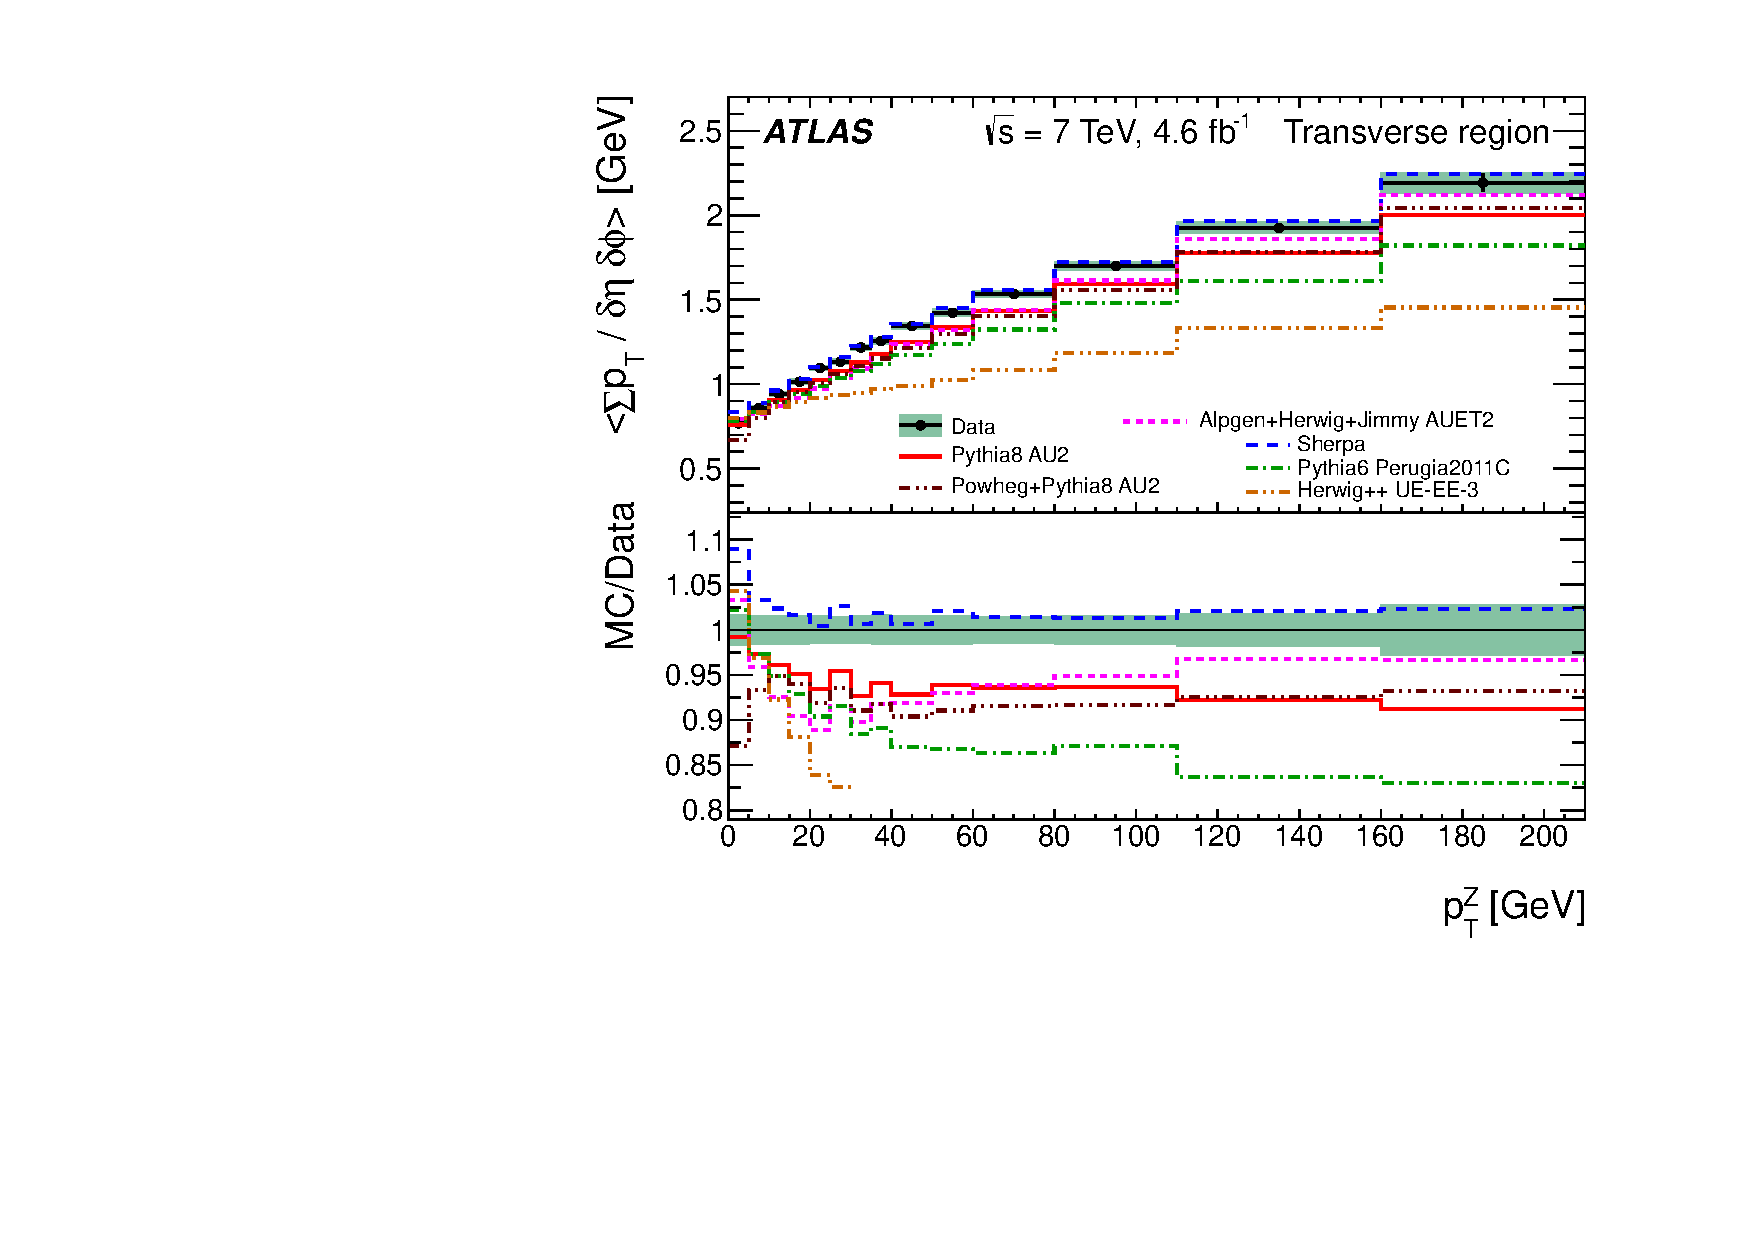
\includegraphics[width=0.48\textwidth]{figures/STDM-2011-42/fig_14b}
  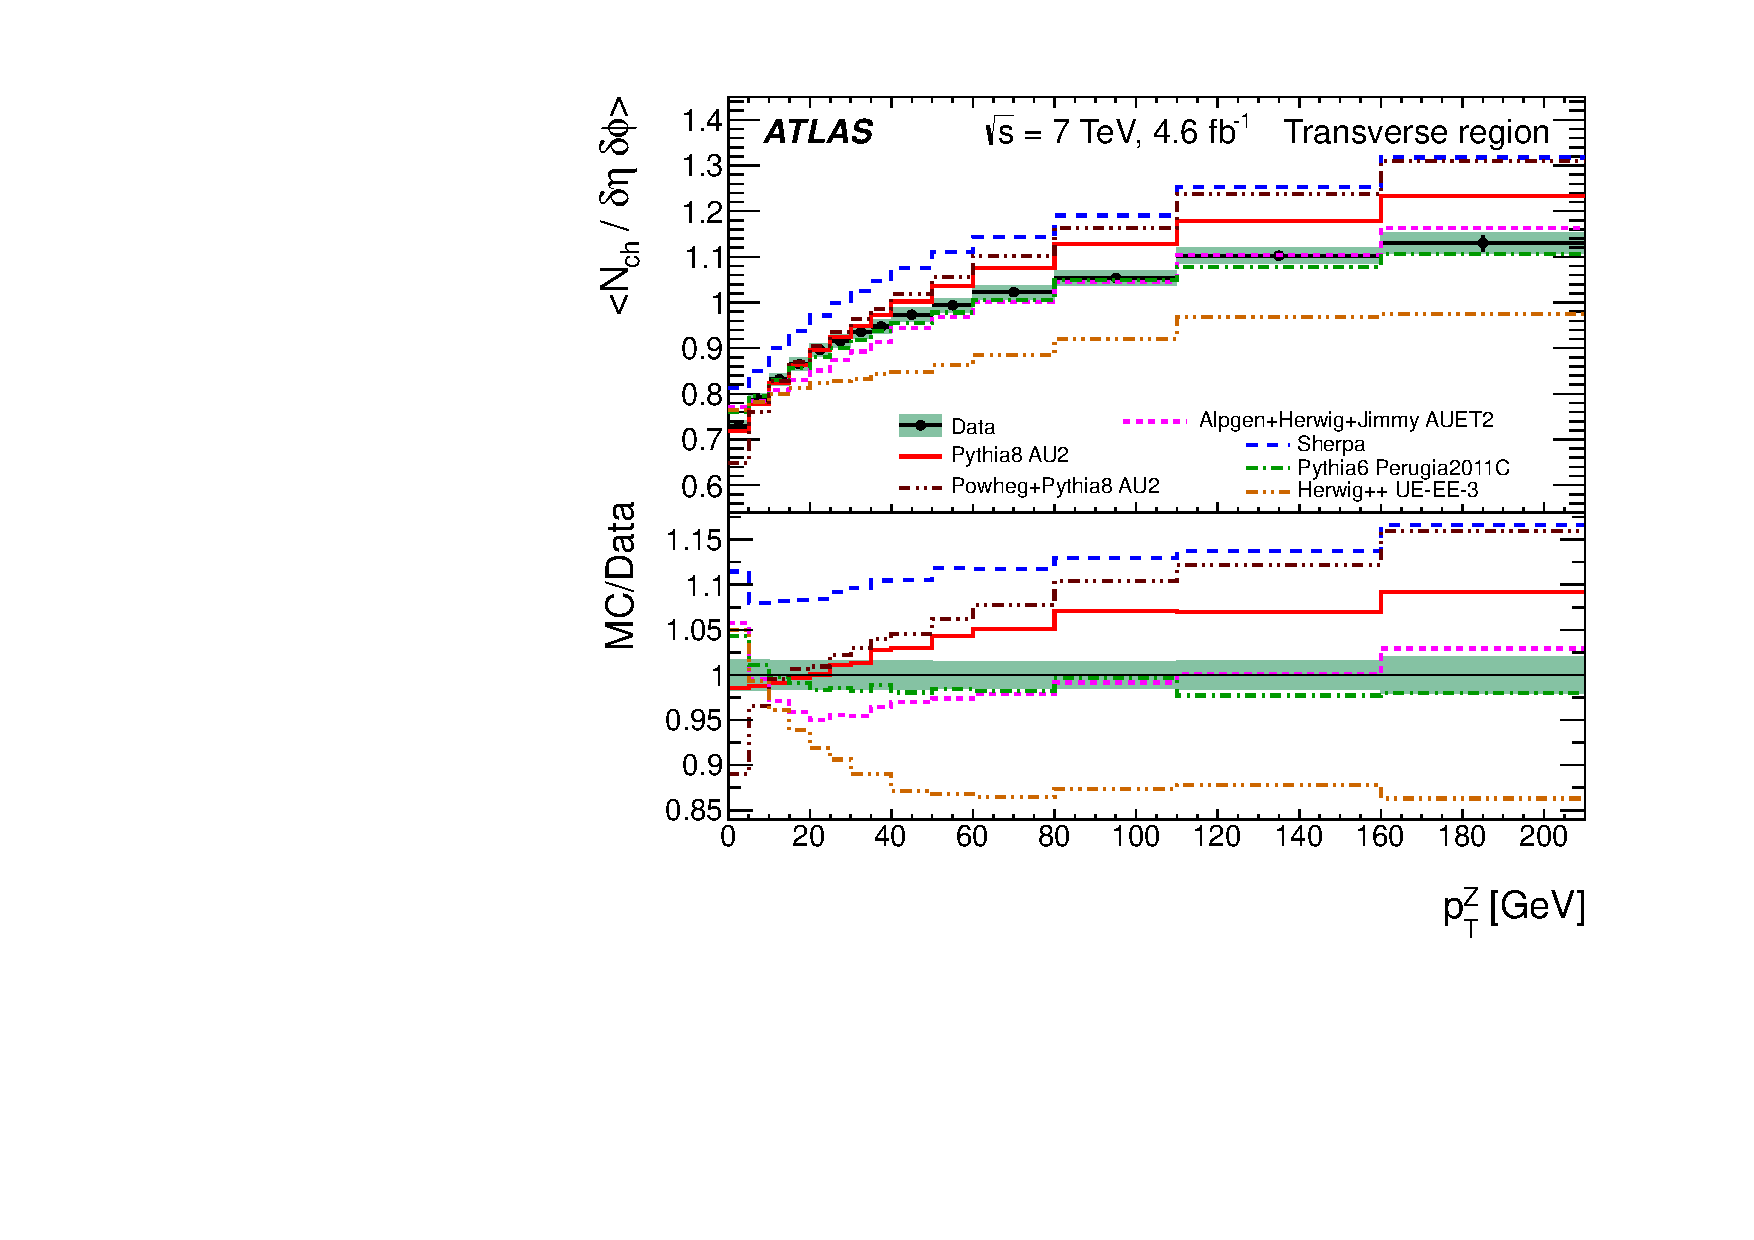
\includegraphics[width=0.48\textwidth]{figures/STDM-2011-42/fig_17b}
  \caption{Comparison of data and various predictions in $\Zll$ events of the charged particle scalar momentum density (left) and multiplicity density (right) as a function of $\pt^Z$ in 2011 data-taking~\cite{STDM-2011-42}. Mis-modeling is observed for all predictions.}
  \label{fig:backgrounds-zue}
\end{figure}

\begin{figure}[tp]
  \centering
  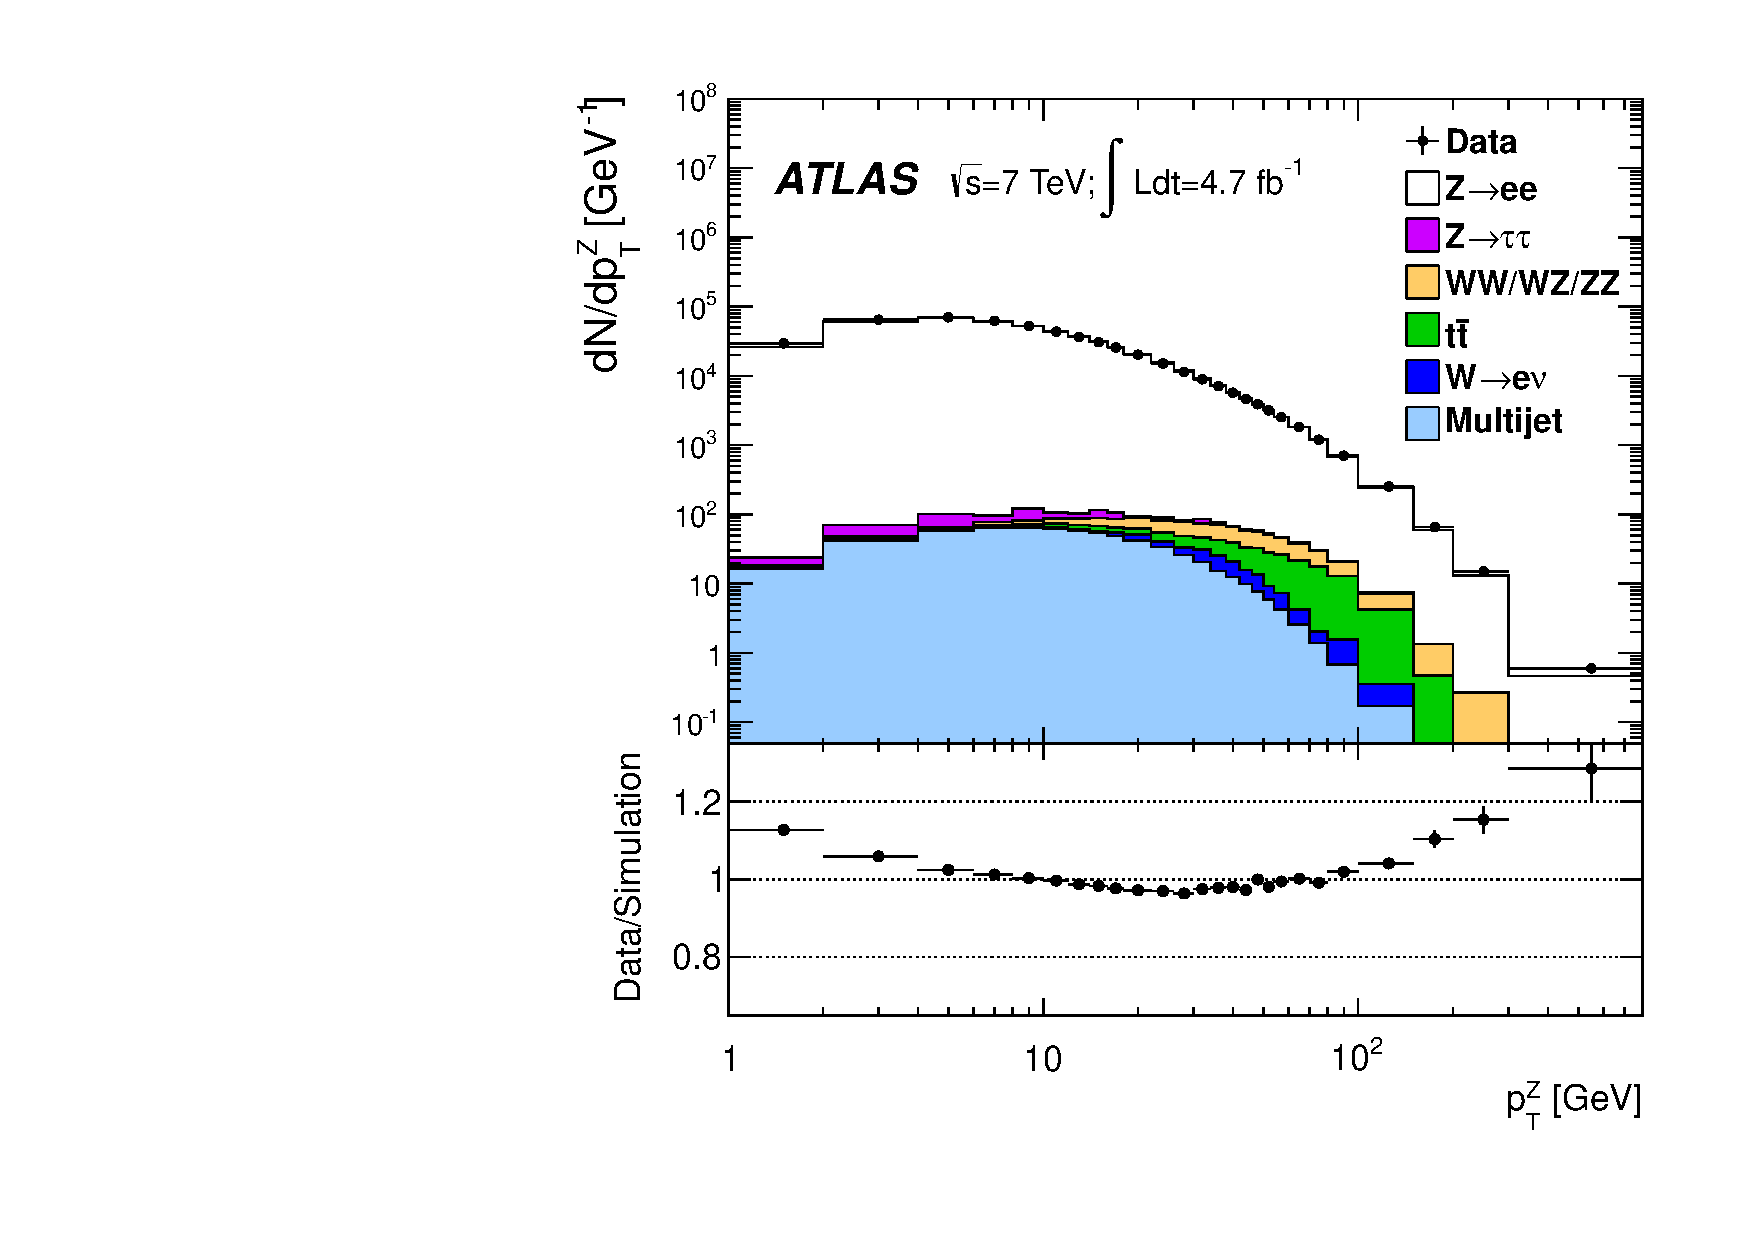
\includegraphics[width=0.48\textwidth]{figures/STDM-2012-23/fig_01a}
  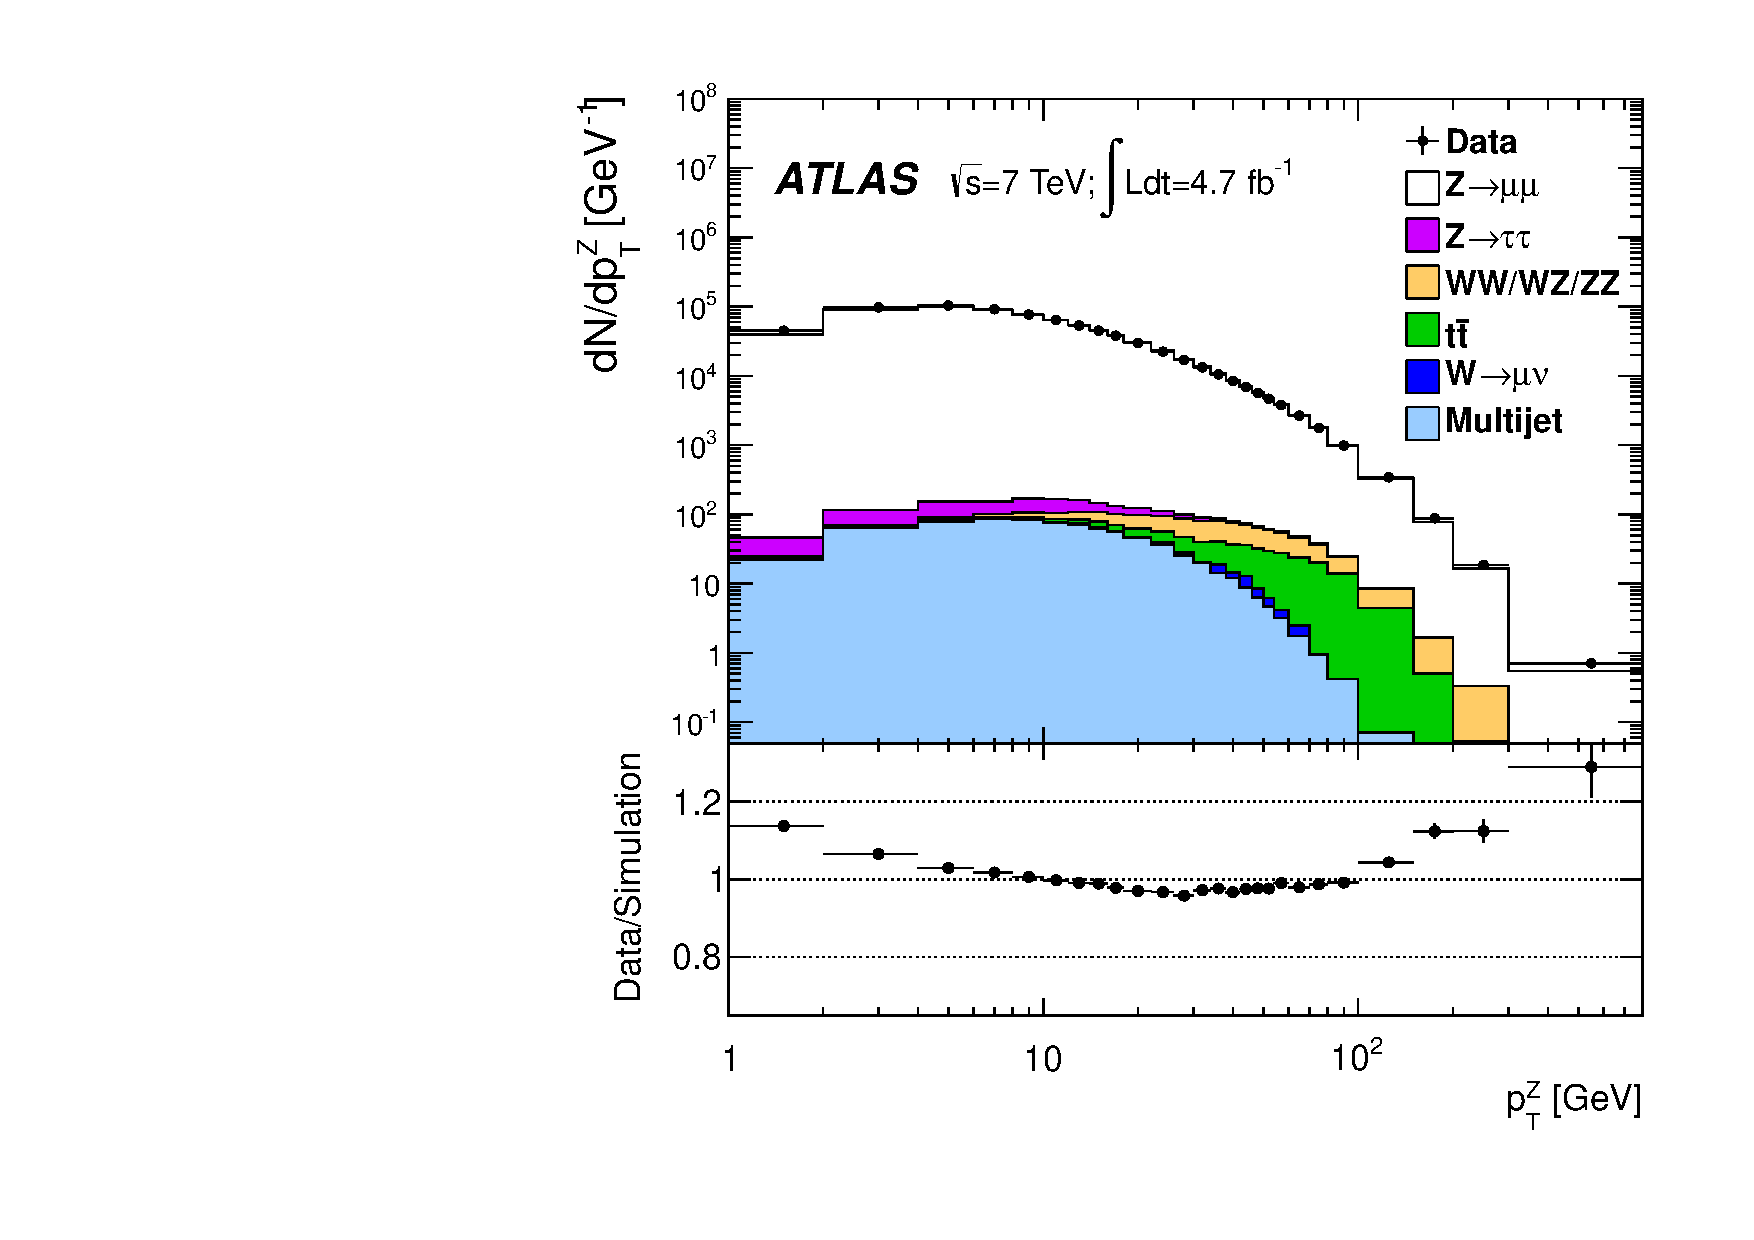
\includegraphics[width=0.48\textwidth]{figures/STDM-2012-23/fig_01b}
  \caption{Comparison of data and various predictions of $\pt^Z$ for $\Zee$ (left) and $\Zmm$ (right) in 2011 data-taking~\cite{STDM-2012-23}. Mis-modeling is observed.}
  \label{fig:backgrounds-zpt}
\end{figure}

\begin{figure}[tp]
  \centering
  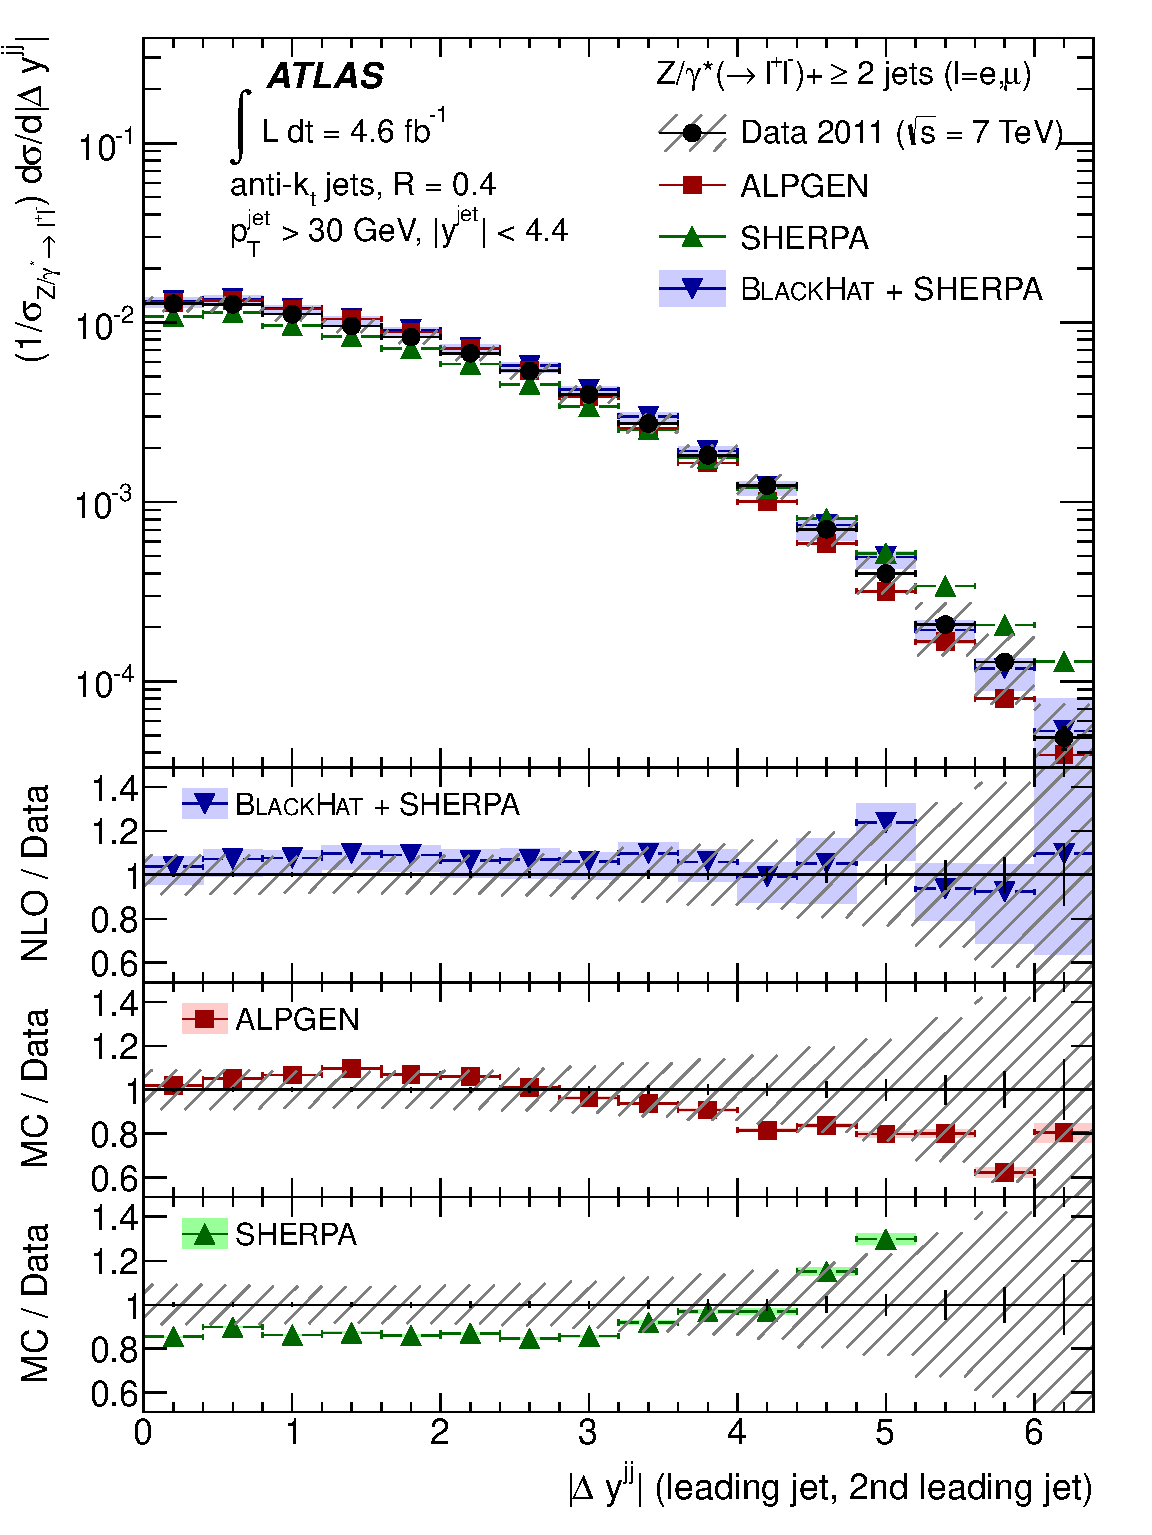
\includegraphics[width=0.48\textwidth]{figures/STDM-2012-04/fig_11a}
  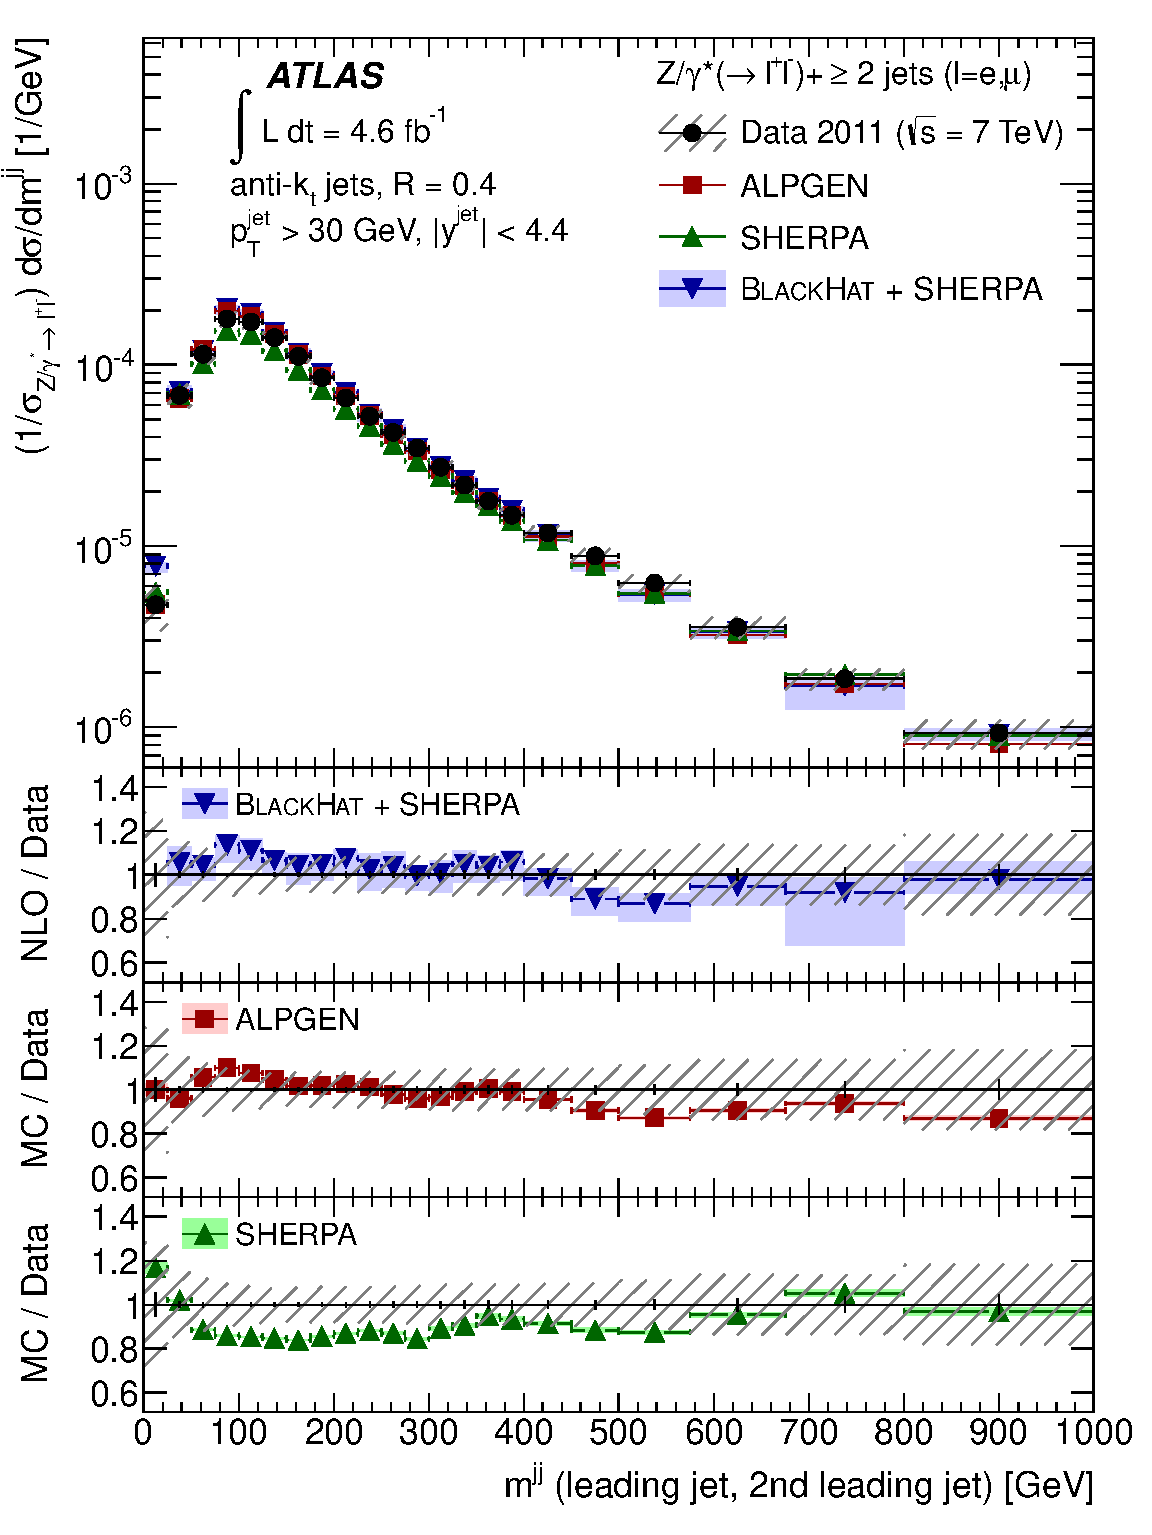
\includegraphics[width=0.48\textwidth]{figures/STDM-2012-04/fig_11b}
  \caption{Comparison of data and various predictions in $\Zll$ events of $\Delta Y(jj)$ (left) and $\mjj$ (right) in 2011 data-taking~\cite{STDM-2012-04}. Mis-modeling is observed for all predictions.}
  \label{fig:backgrounds-zjj}
\end{figure}

These mis-modelings are worrisome for $\Htautau$ analyses because accurate modeling of these kinematics is relied on in the analysis. For example, mis-modeling in $\pt^Z$ is problematic because this variable defines the boosted category of the $\Htautau$ analysis. It is also strongly correlated with discriminating variables like $\Delta R(\tautau)$. Mis-modeling in dijet kinematics like $\mjj$ is of even greater concern because they are among the most powerful and high-profile discriminating variables in the VBF category.

Some versions of the ATLAS $\Htautau$ analysis use simulated $\Ztautau$ with corrections derived from $\Zll$ events in data~\cite{ATLAS-CONF-2012-160}. While helpful, these corrections are one-dimensional and cannot account for potential correlations in the mis-modeling. For these reasons, this approach is not used in the recent publication.

\subsection{Embedding}

A more data-driven approach to modeling $\Ztautau$ is used wherein $\Zmumu$ events are tagged in data and the muons are replaced with simulated tau lepton decays. This exploits lepton universality in $Z$ decays and has the great advantage of taking all $Z\!+\text{jets}$ features directly from data, such as $Z$ $\pt$, dijet kinematics, and soft hadronic activity. Only the tau lepton decays and the detector response of the decay products are taken from simulation. The former is measured with excellent precision at $B$-factories~\cite{2014.hfag}, and the latter is an ongoing area of study within ATLAS.

$\Zmumu$ events are selected in data by requiring an event fire the lowest unprescaled dimuon trigger and have at least two reconstructed muons with $\pt > 15$ GeV and $|\eta| <$ 2.5. All possible pairs of muons are then considered which satisfy $\pt^\text{lead} > $ 20 GeV, have opposite charges, and have $m_{\mu\mu} > $ 40 GeV. The pair which has mass closest to the $Z$ mass is then chosen as the $Z$ decay products.

Tau lepton decays are then simulated with \texttt{TAUOLA} with the same four-momenta as the muons associated to the $Z$ decay and sent through the full ATLAS detector simulation, digitization, and reconstruction. The decays can be set to whatever final state desired (e.g., $\tautaueh$) within \texttt{TAUOLA}. 

The simulated $\tautau$ system is then merged with the data $\Zmumu$ event by removing tracks and calorimeter cells associated to the muons and inserting tracks and cells from the tau lepton decays. For subtracting the calorimeter cells, deposited cell energies are derived from a simulated $\Zmumu$ event with the same kinematics as the data $\Zmumu$ event. The hybrid event, with a simulated $\tautau$ system and a $Z\!+\text{jets}$ event from data, is then re-run through the ATLAS reconstruction, yielding the so-called \textit{embedded} $\Ztautau$ event. Event displays of this procedure is shown in \cref{fig:backgrounds-embedding-eventdisplay}.

\begin{figure}[tp]
  \centering
  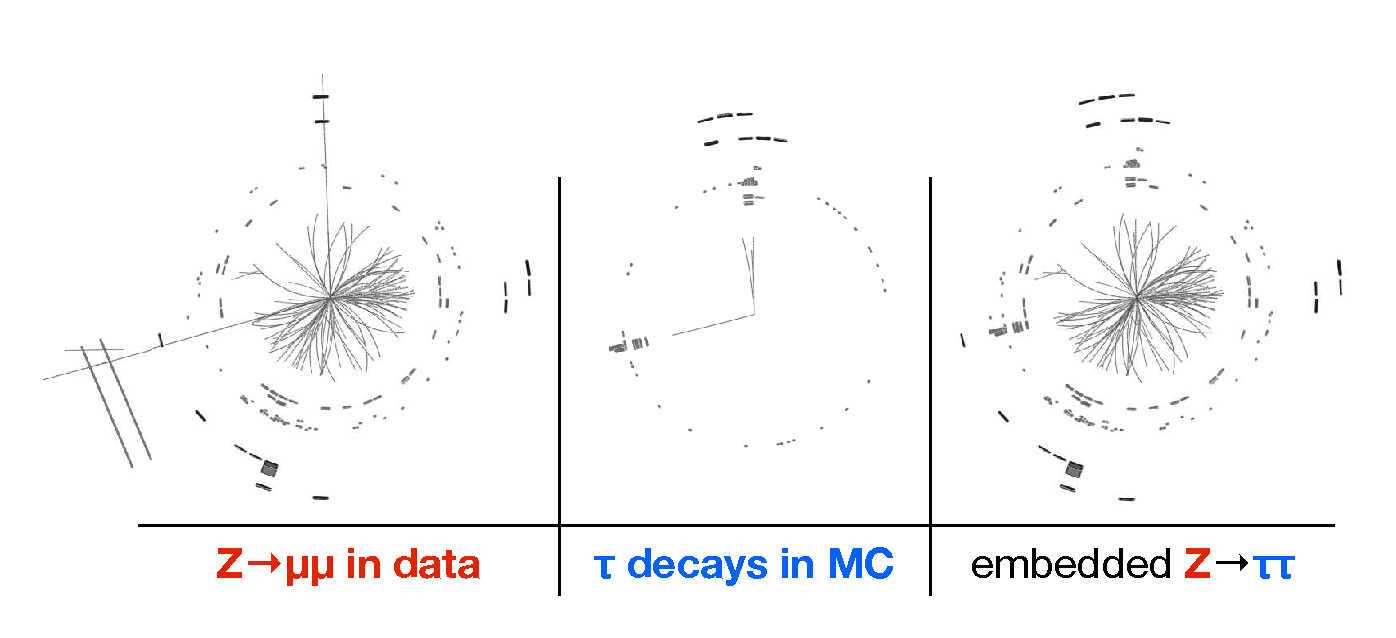
\includegraphics[width=0.95\textwidth]{figures/backgrounds/embedding_eventdisplay}
  \caption{Event displays of the three types of events considered in the embedding procedure: a $\Zmumu$ event in data (left), a $\tautauhh$ event in simulation (center), and a hybrid embedding event (right)~\cite{ATL-COM-PHYS-2012-1201}.}
  \label{fig:backgrounds-embedding-eventdisplay}
\end{figure}

\subsection{Validation}

\begin{figure}[tp]
  \centering
  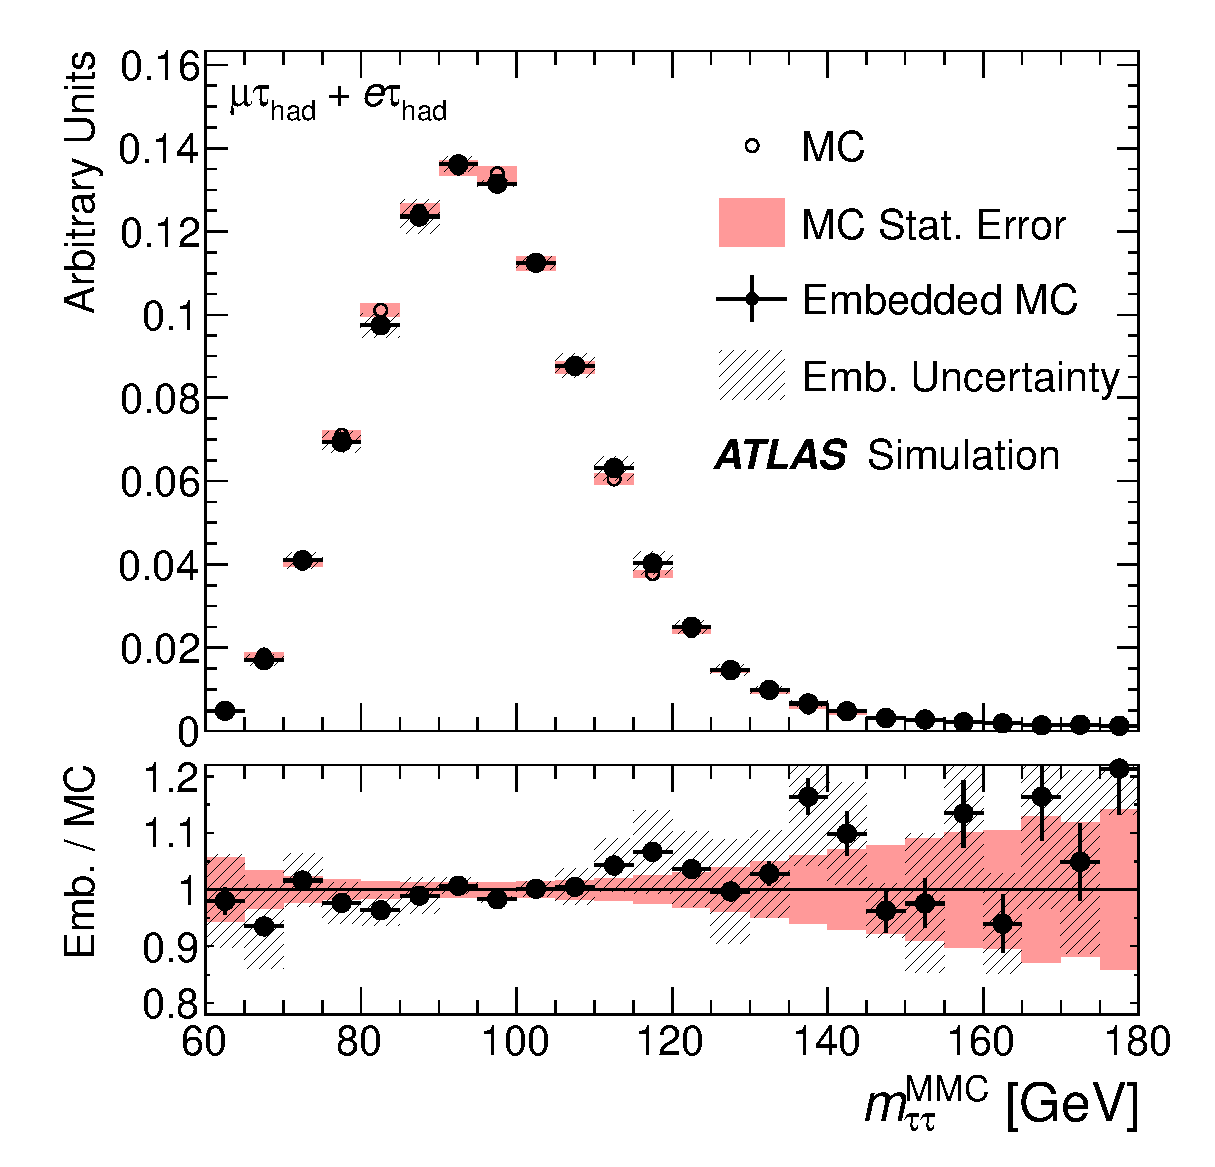
\includegraphics[width=0.48\textwidth]{figures/HIGG-2013-32/fig_03b}
  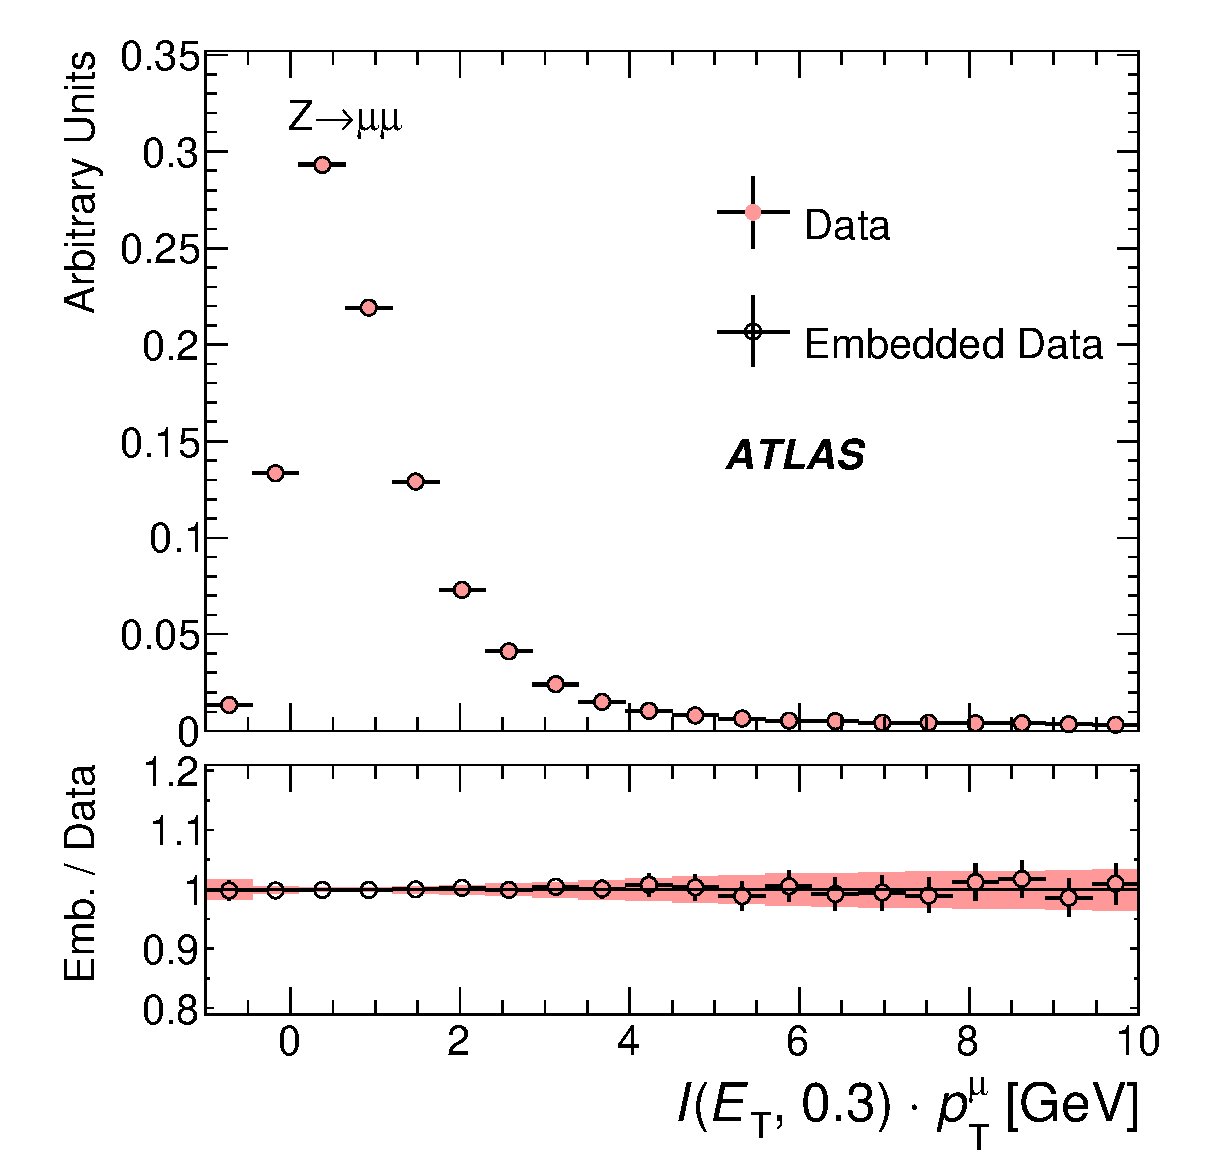
\includegraphics[width=0.48\textwidth]{figures/HIGG-2013-32/fig_03a}
  \caption{Validation of the embedding technique for simulated tau lepton decays in simulated $\Zmm$ events (left) and simulated muons in data $\Zmm$ events (right)~\cite{HIGG-2013-32}. Good agreement is observed in both.}
  \label{fig:backgrounds-embedding-validation}
\end{figure}

\clearpage

\subsection{Uncertainties}

\begin{figure}[tp]
  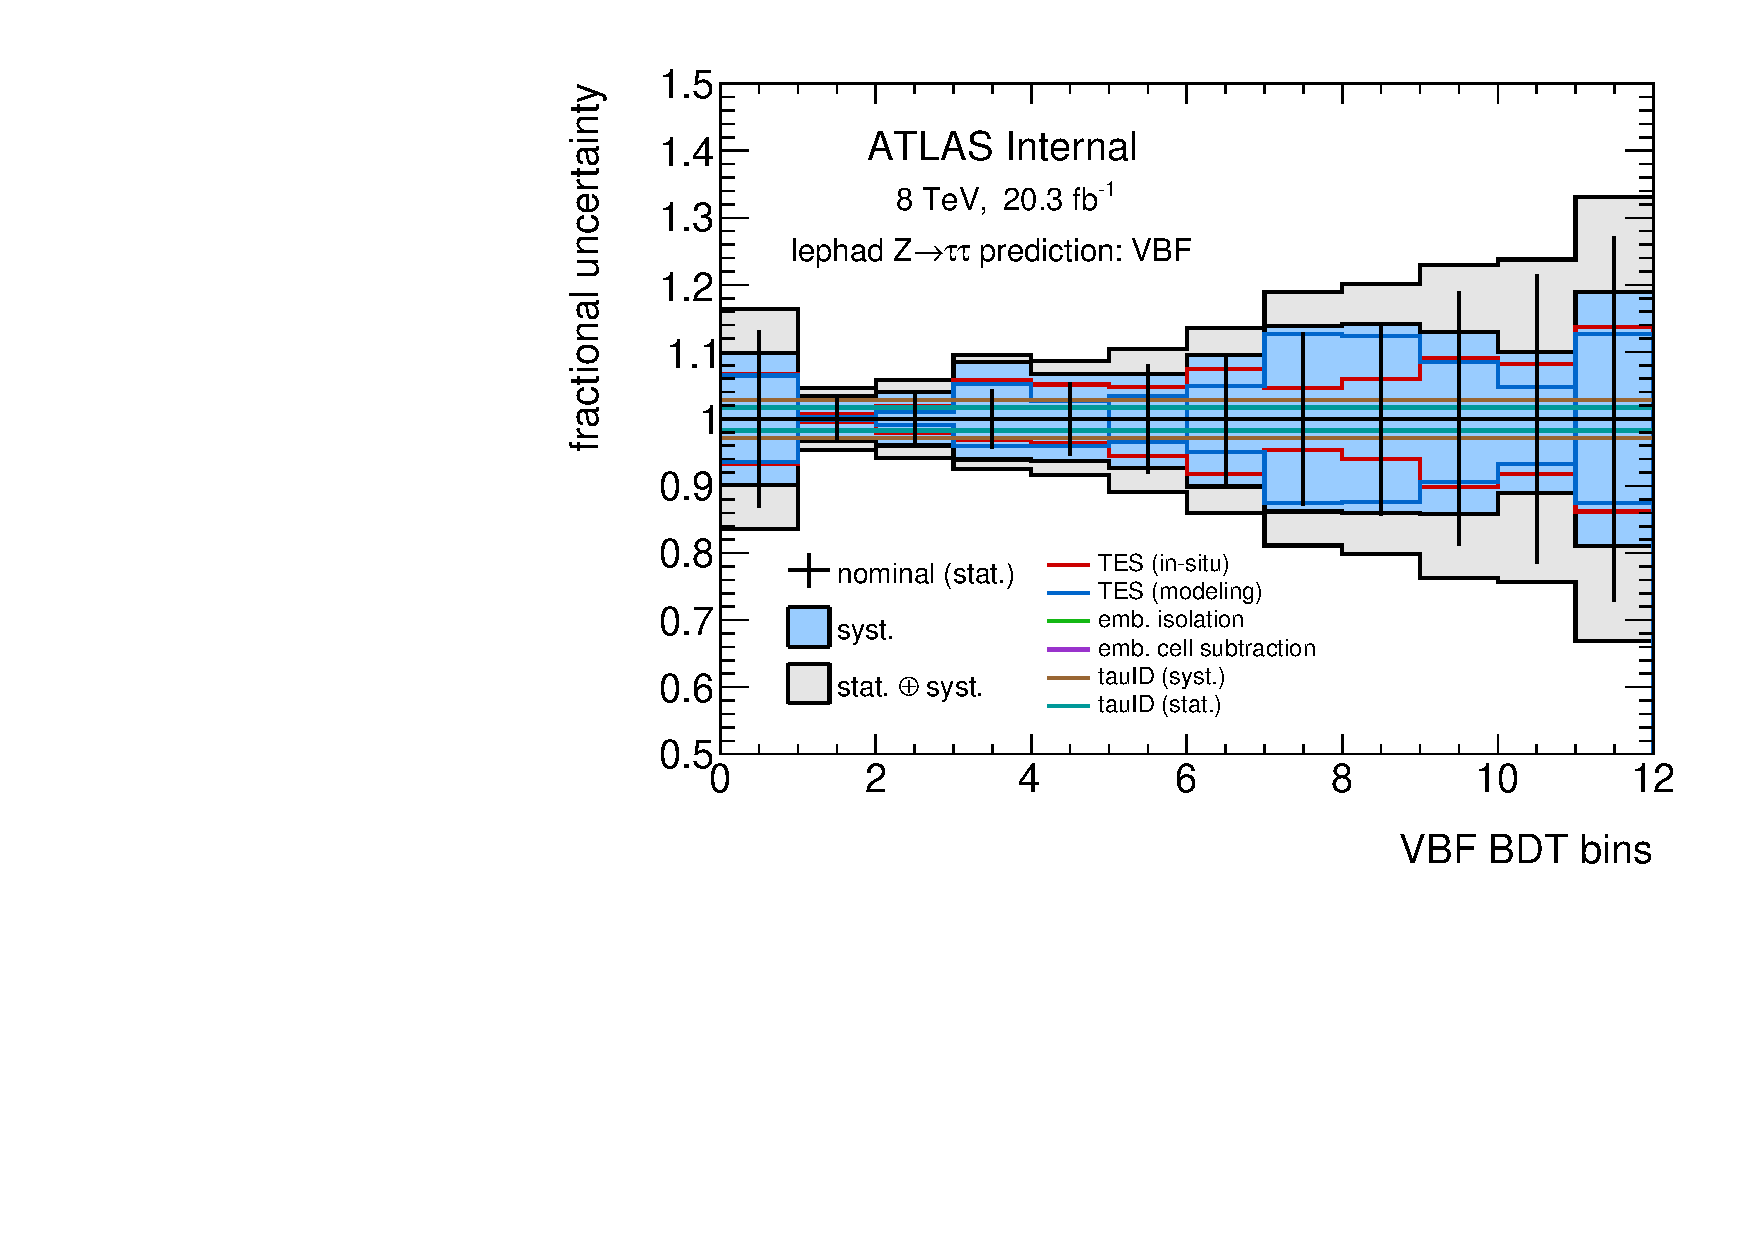
\includegraphics[width=0.90\textwidth]{figures/uncertainties/uncertainties_lephad_paper14_8TeV_Ztautau_VBF}
  \caption{The fractional uncertainty on the embedded $\Ztautaulh$ prediction in each bin of the VBF category for uncertainties pertaining to the embedding procedure and $\tauh$ performance.}
  \label{fig:backgrounds-uncertainties-Ztautau}
\end{figure}

\clearpage
\section{$\fakes$ mis-identification}
\label{sec:backgrounds-misid}

\subsection{Mis-modeling of $\fakes$ in simulation}

\subsection{Fake factor method}

\begin{figure}[tp]
  \centering
  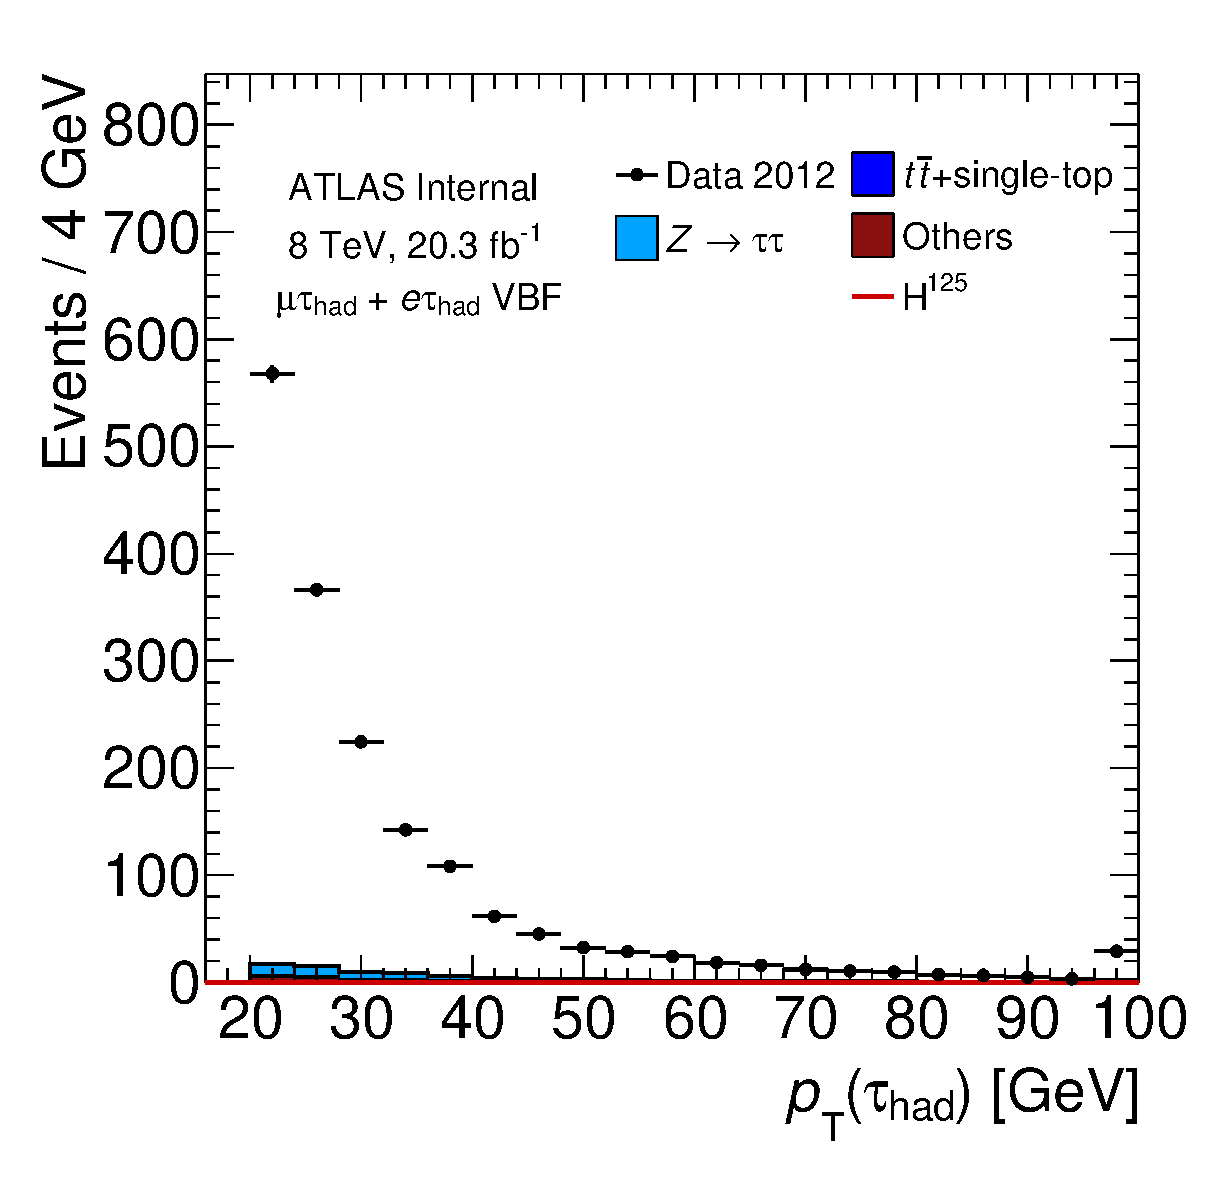
\includegraphics[width=0.32\textwidth]{figures/antitaus/tau-pt}
  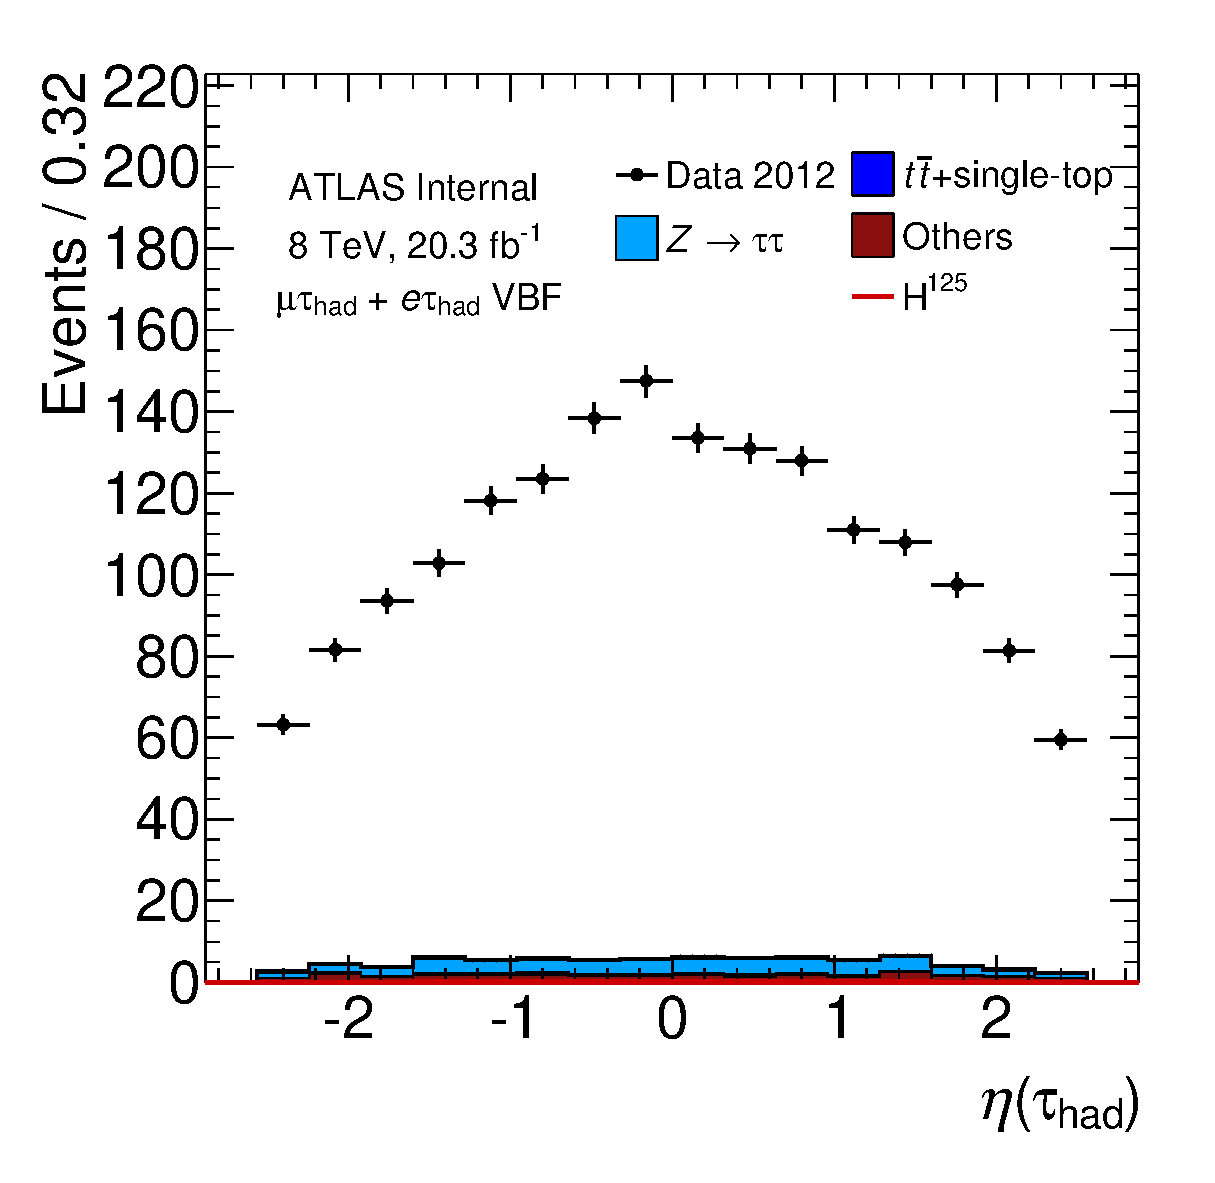
\includegraphics[width=0.32\textwidth]{figures/antitaus/tau-eta}
  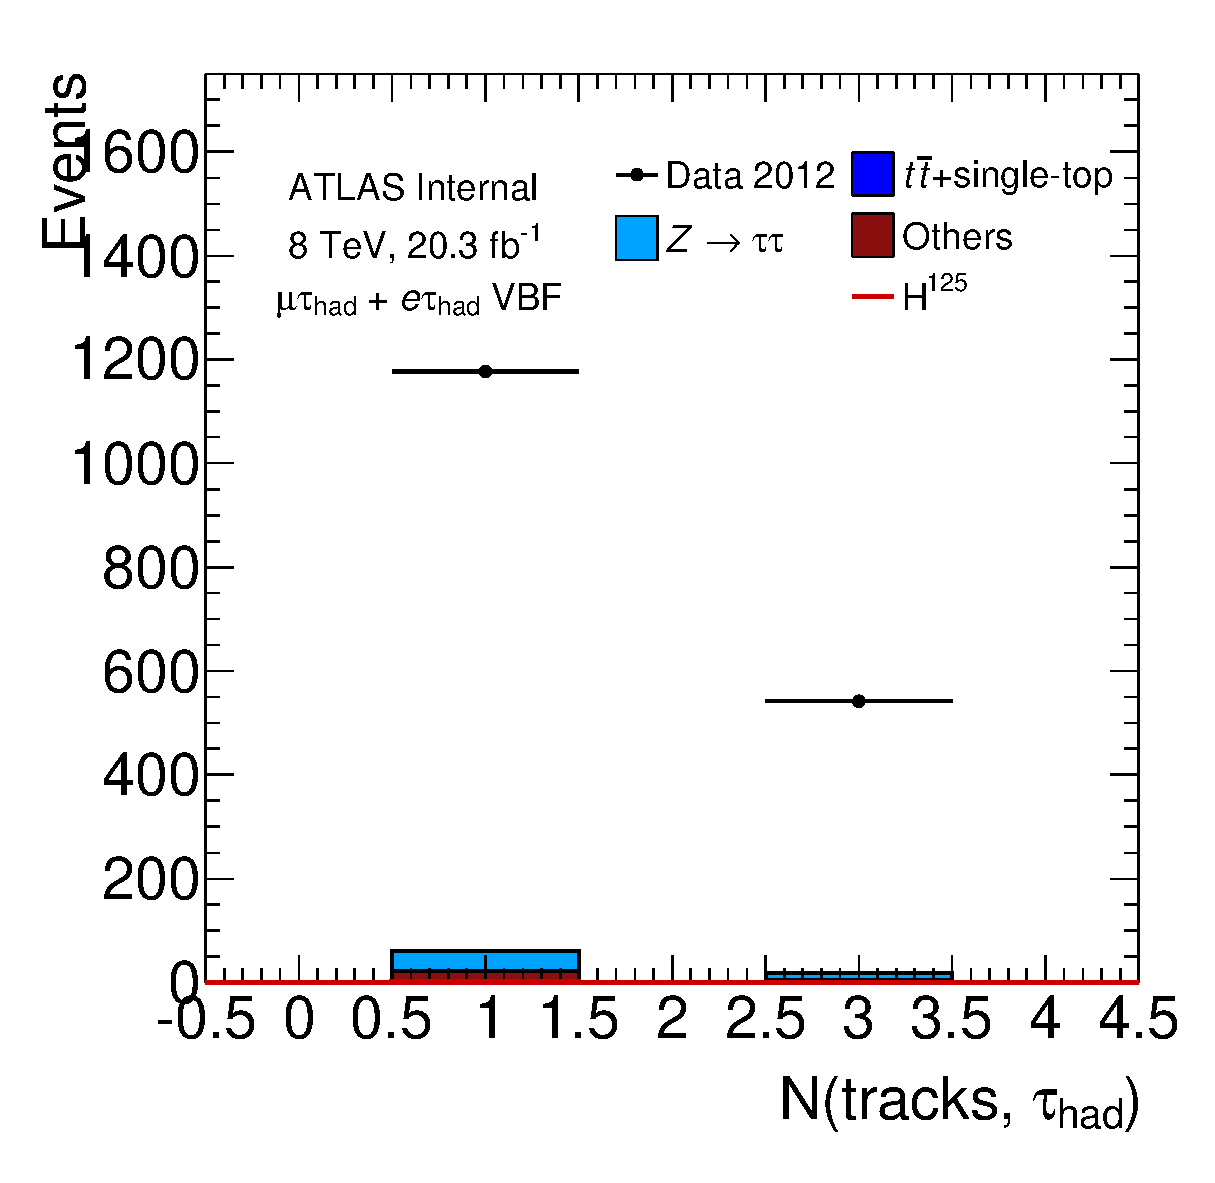
\includegraphics[width=0.32\textwidth]{figures/antitaus/tau-numTrack}
  % --------------
  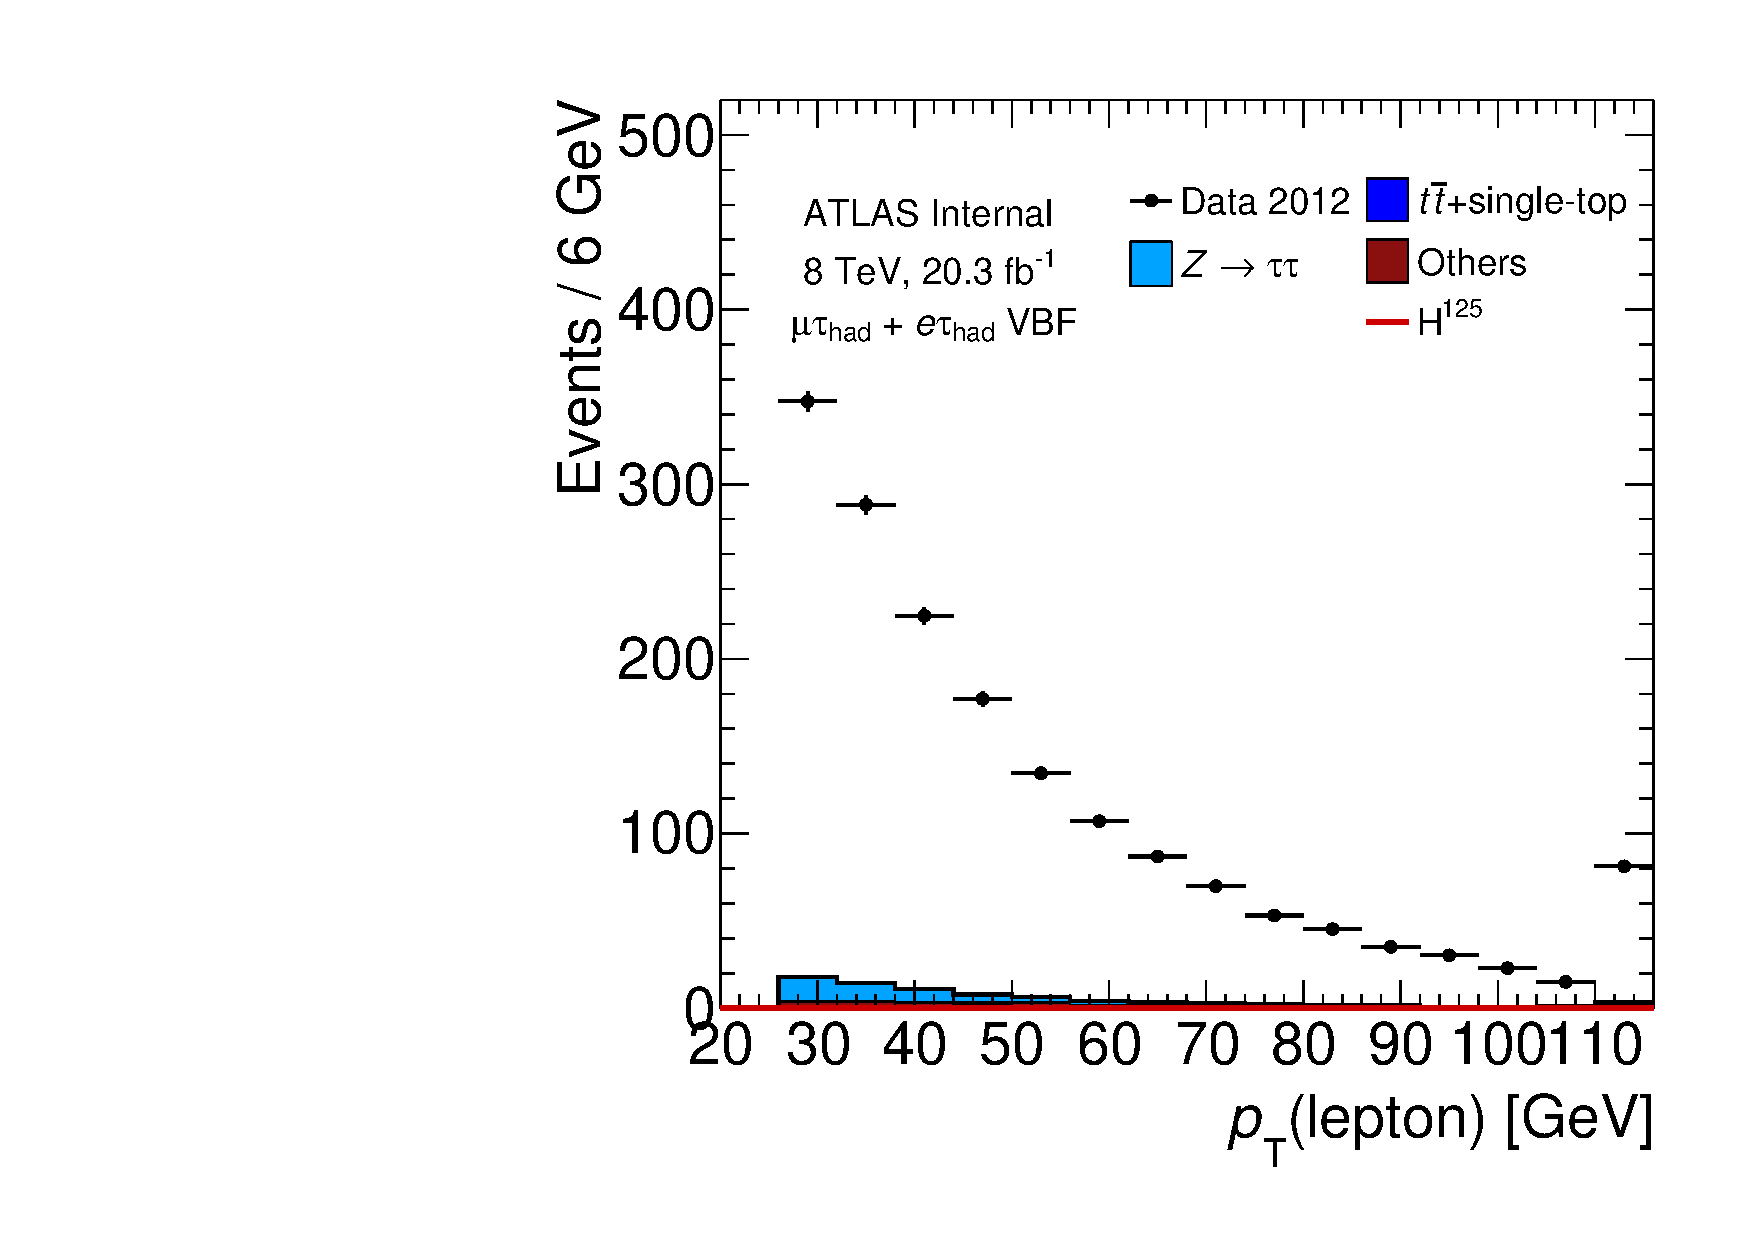
\includegraphics[width=0.32\textwidth]{figures/antitaus/lep-pt-hi}
  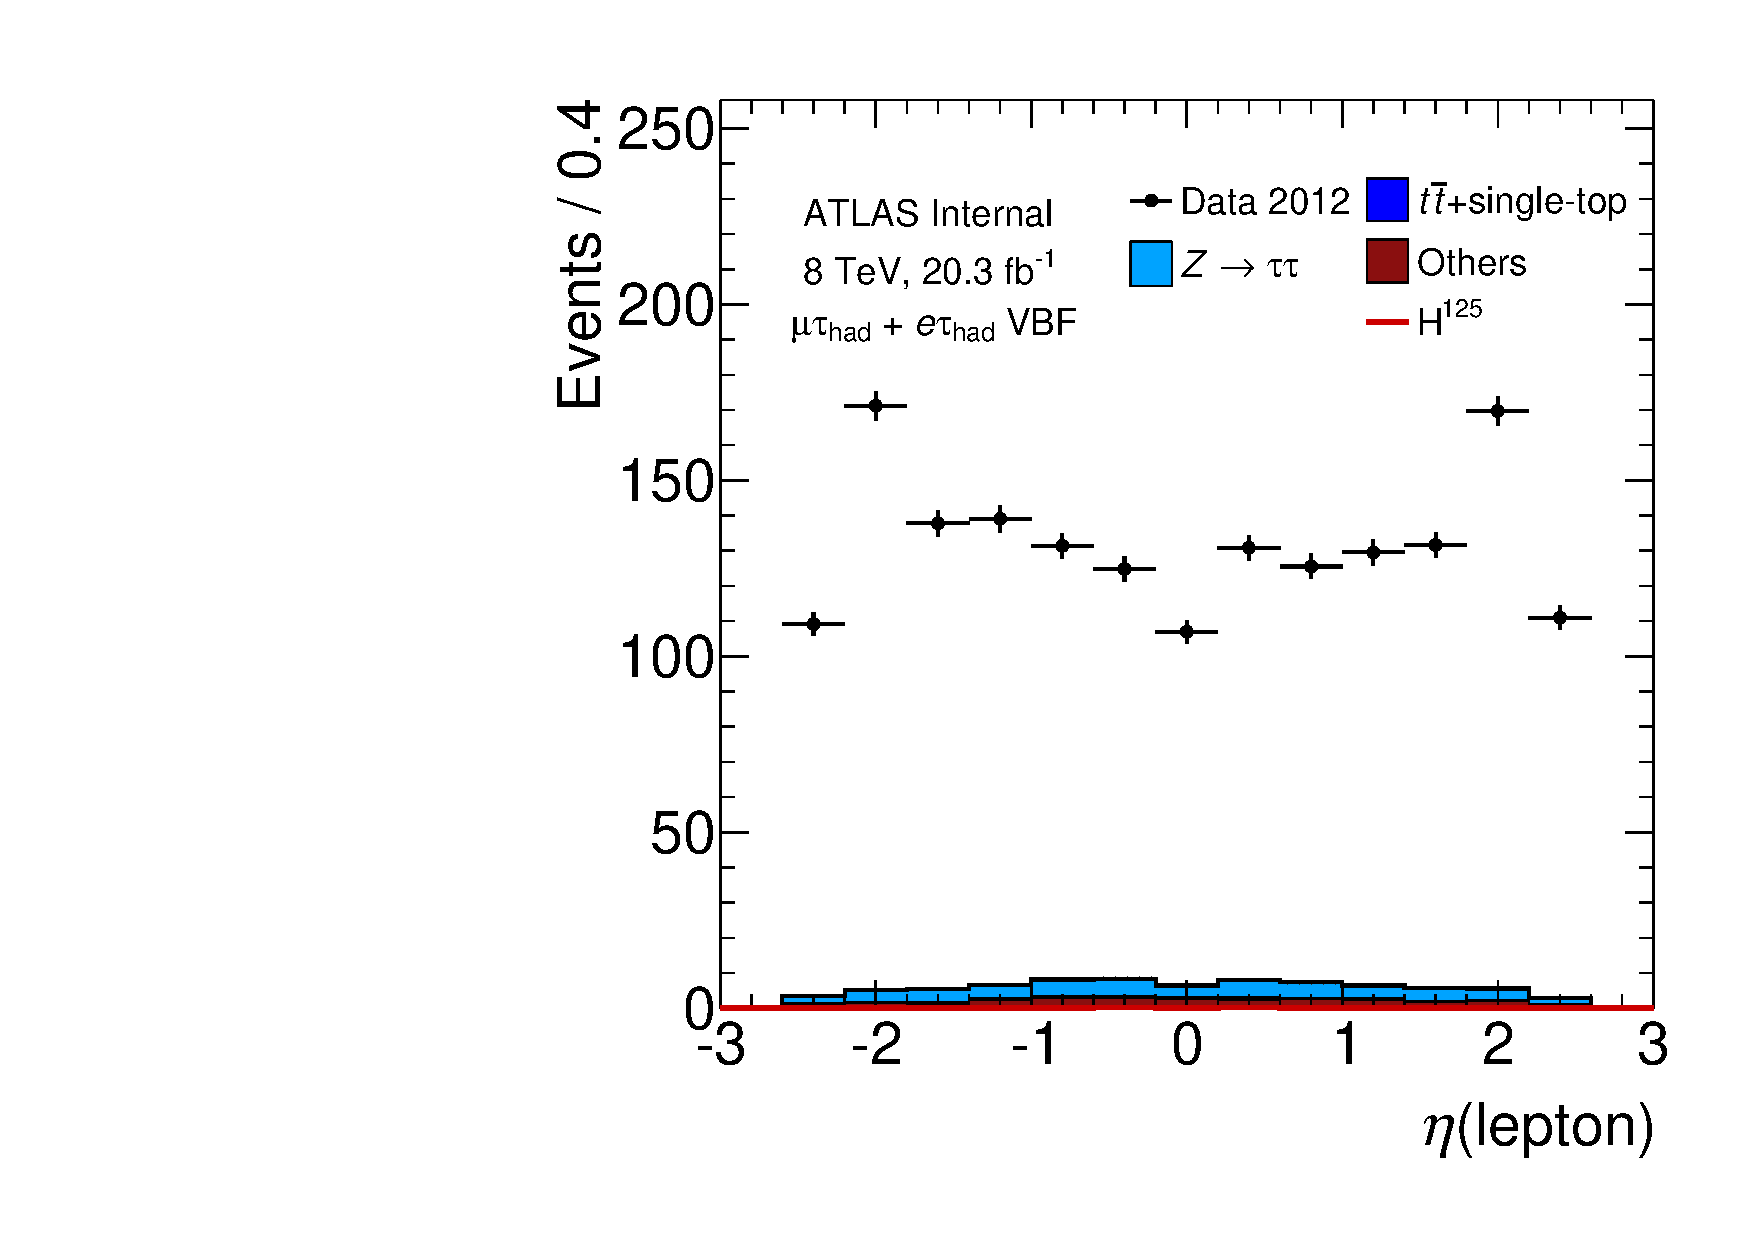
\includegraphics[width=0.32\textwidth]{figures/antitaus/lep-eta}
  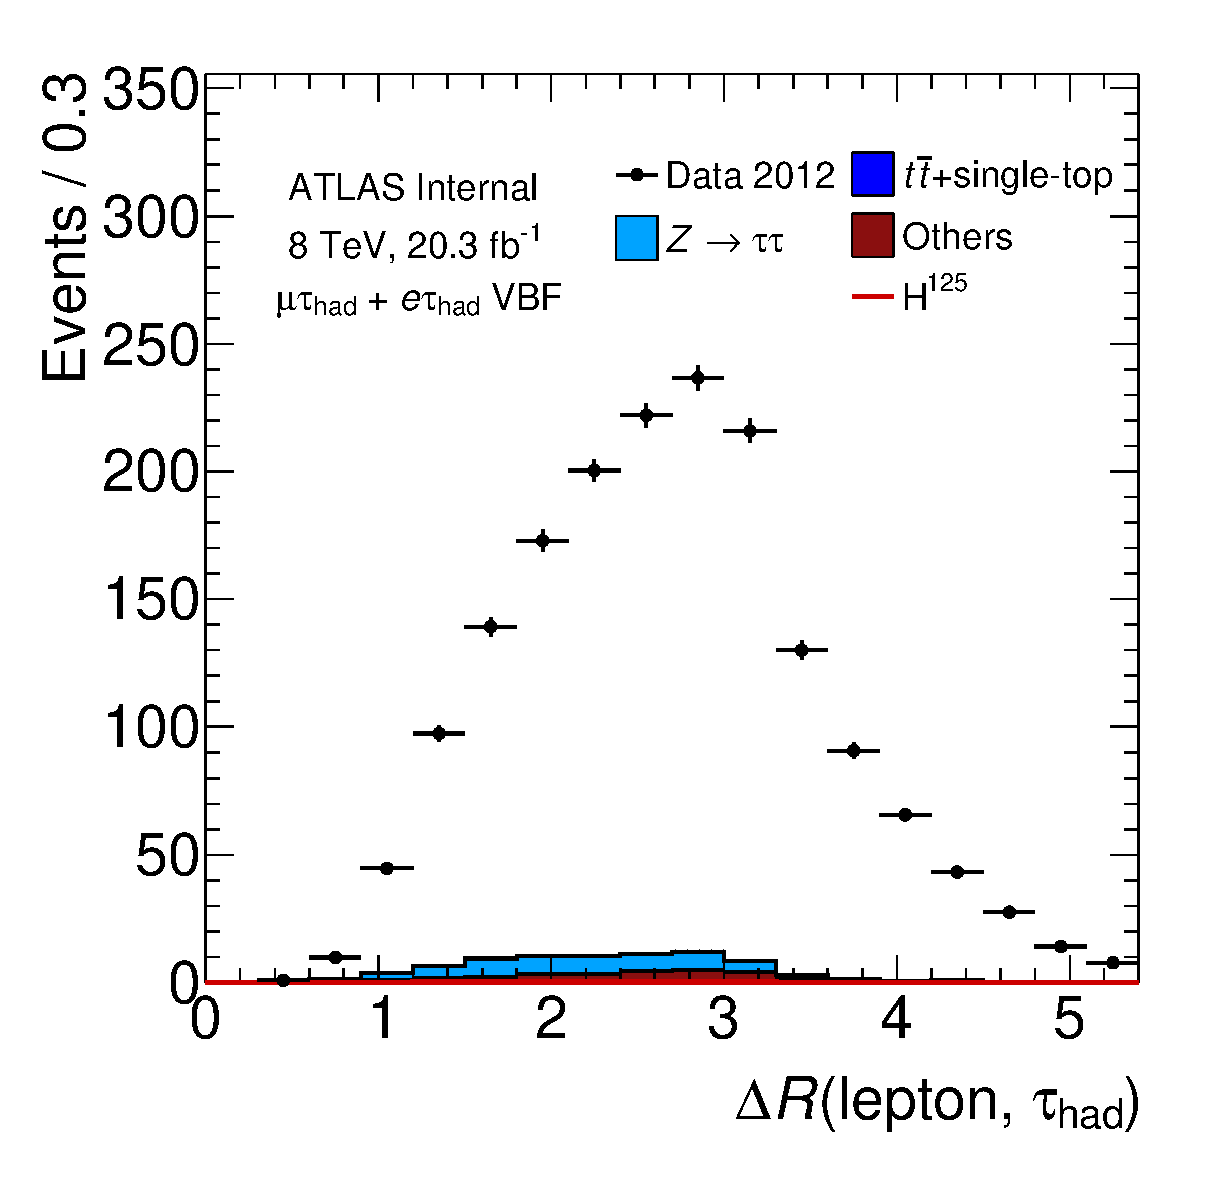
\includegraphics[width=0.32\textwidth]{figures/antitaus/taulep-dR}
  % --------------
  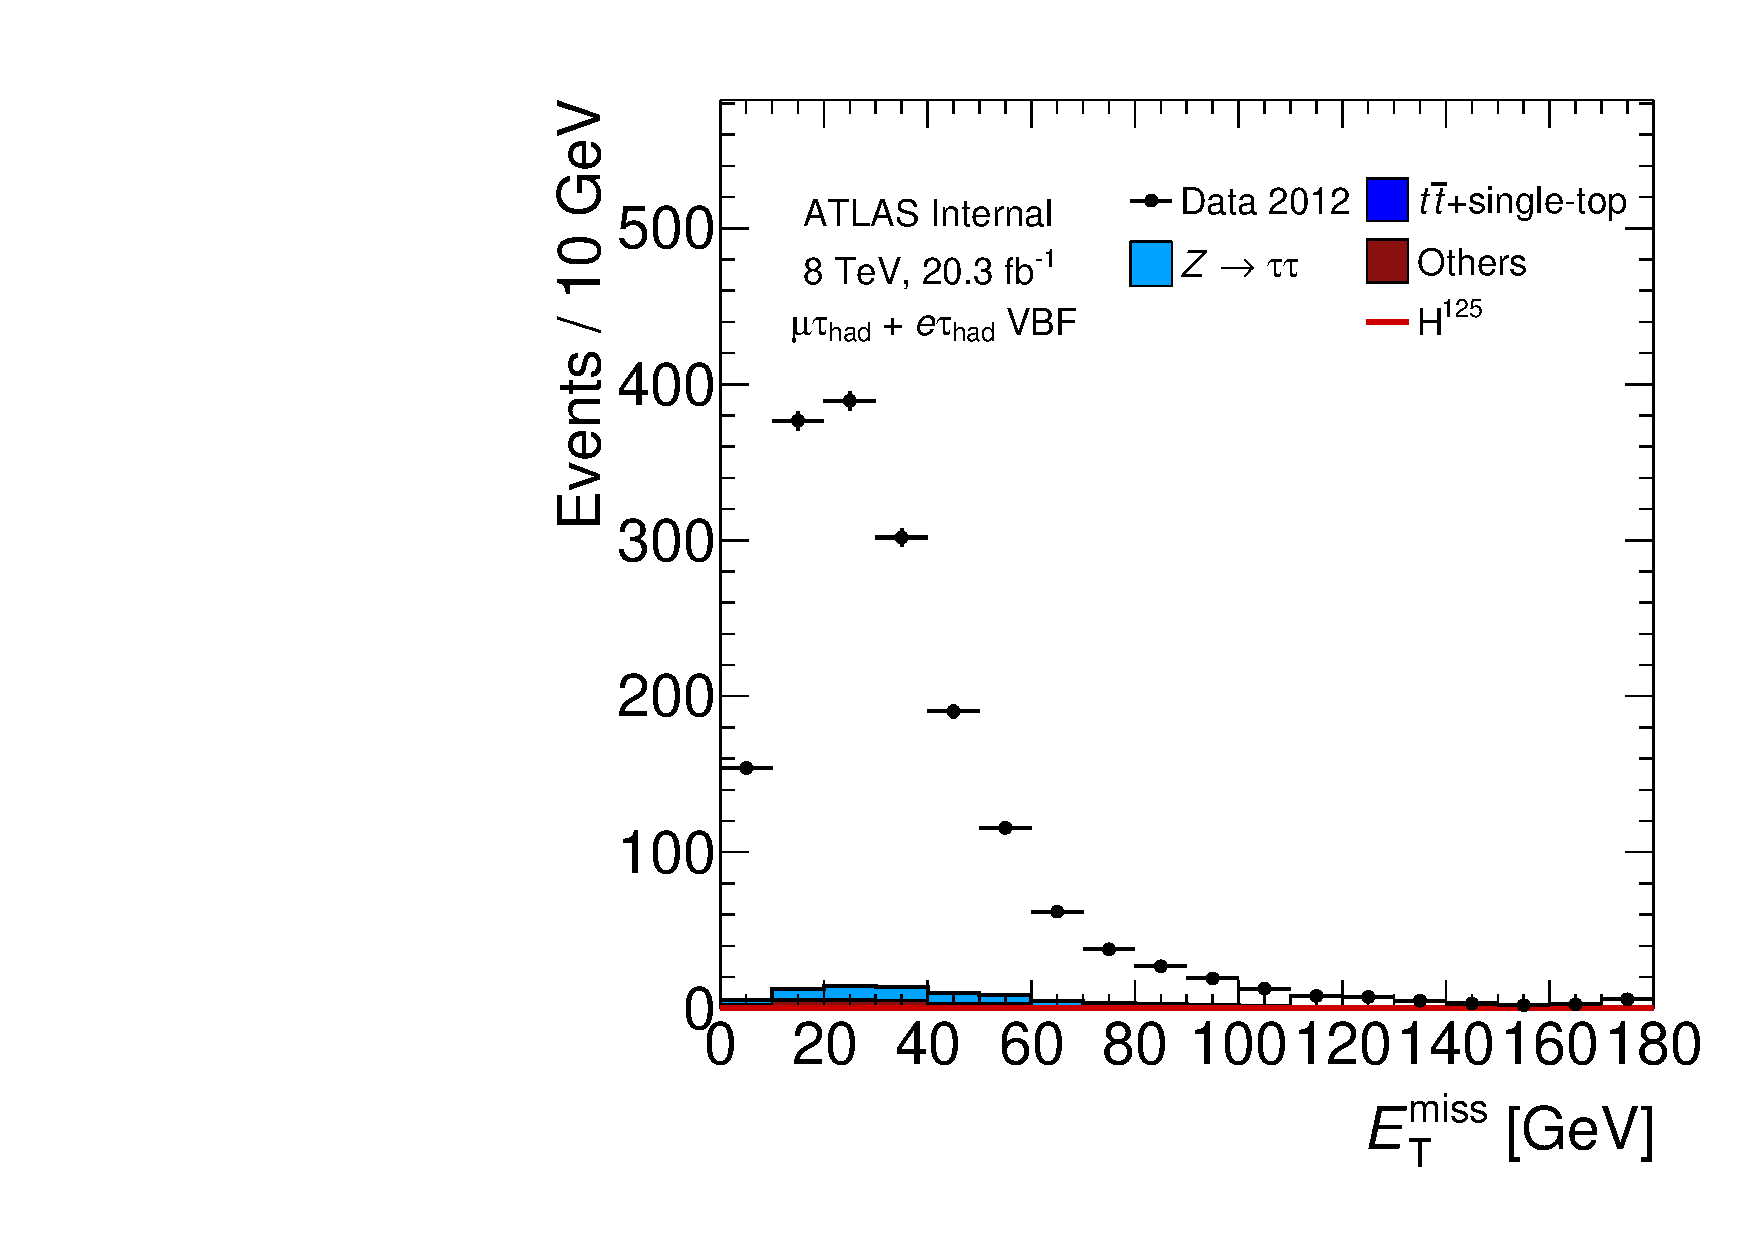
\includegraphics[width=0.32\textwidth]{figures/antitaus/met-pt-hi}
  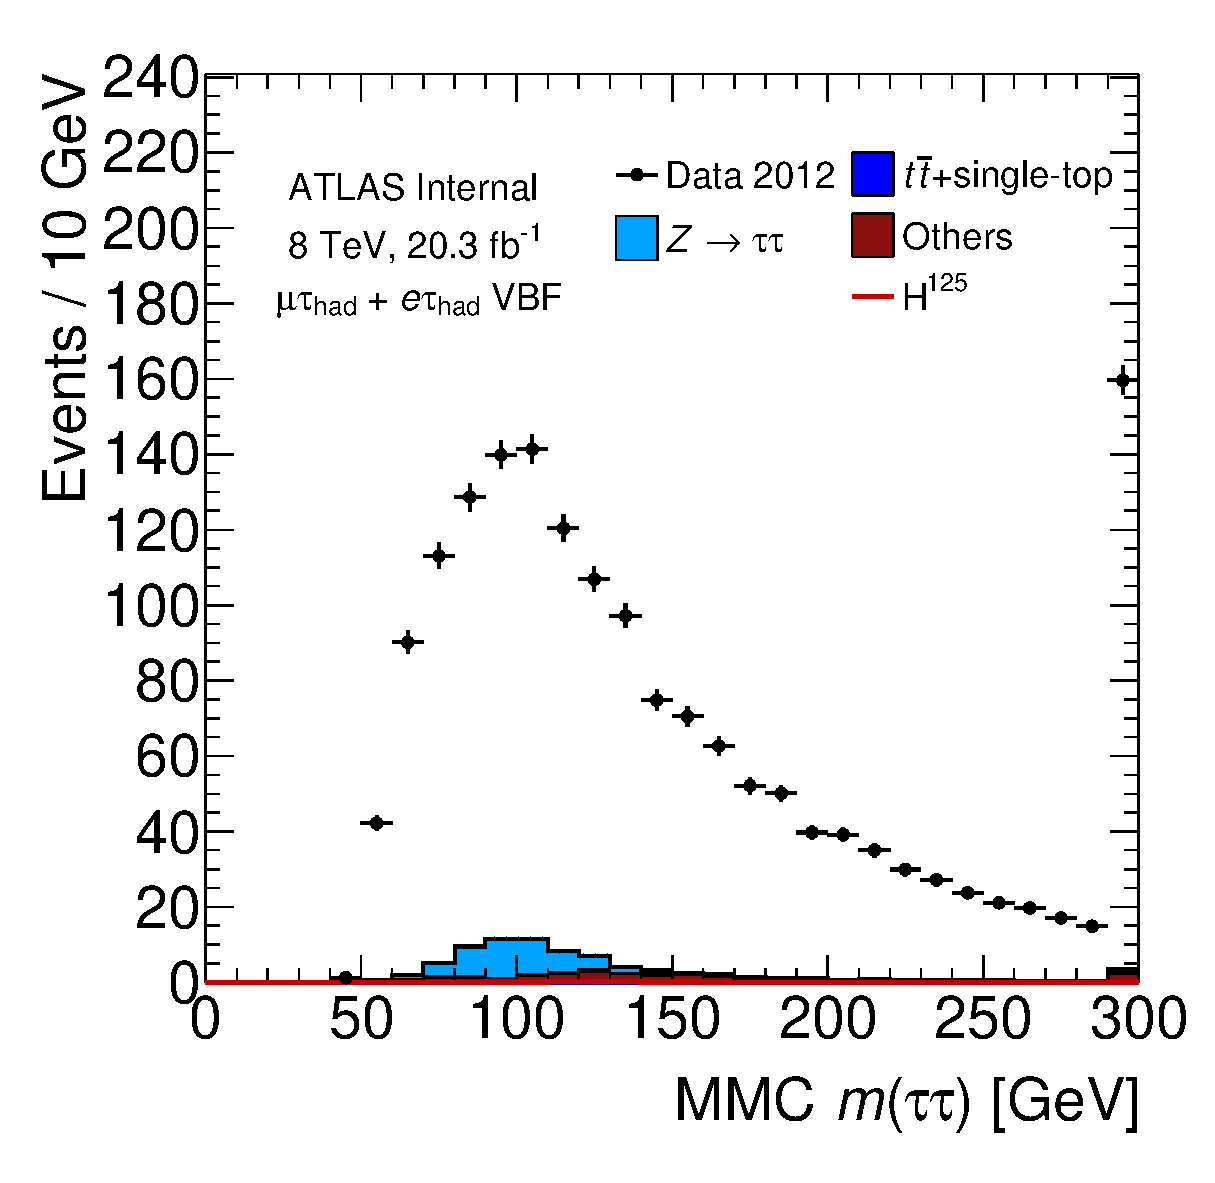
\includegraphics[width=0.32\textwidth]{figures/antitaus/mMMC}
  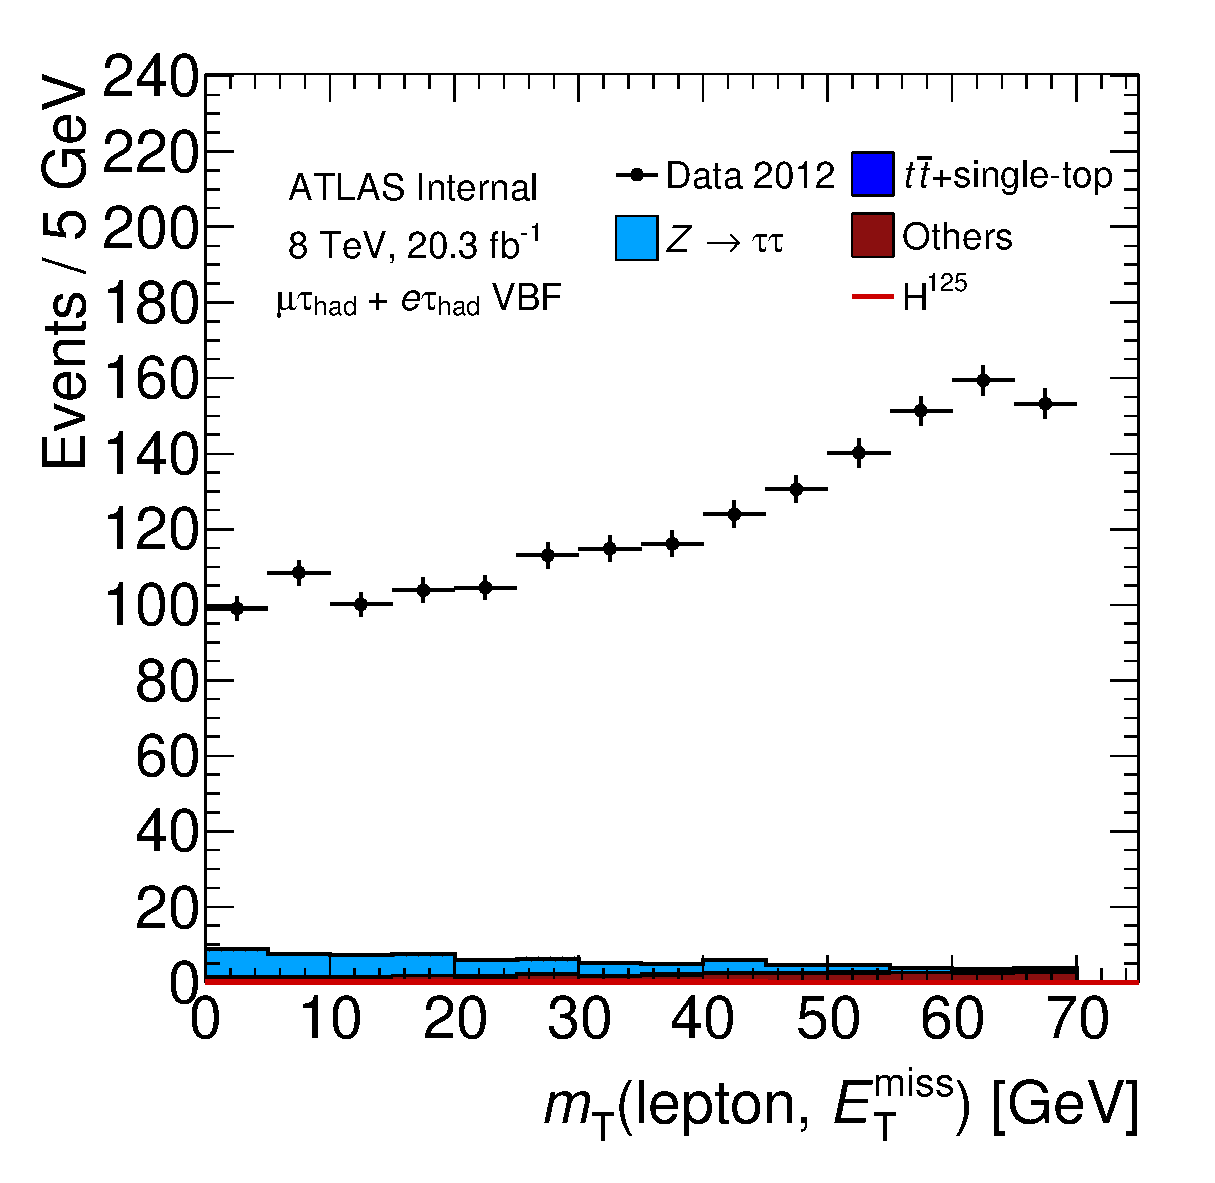
\includegraphics[width=0.32\textwidth]{figures/antitaus/mT}
  % --------------
  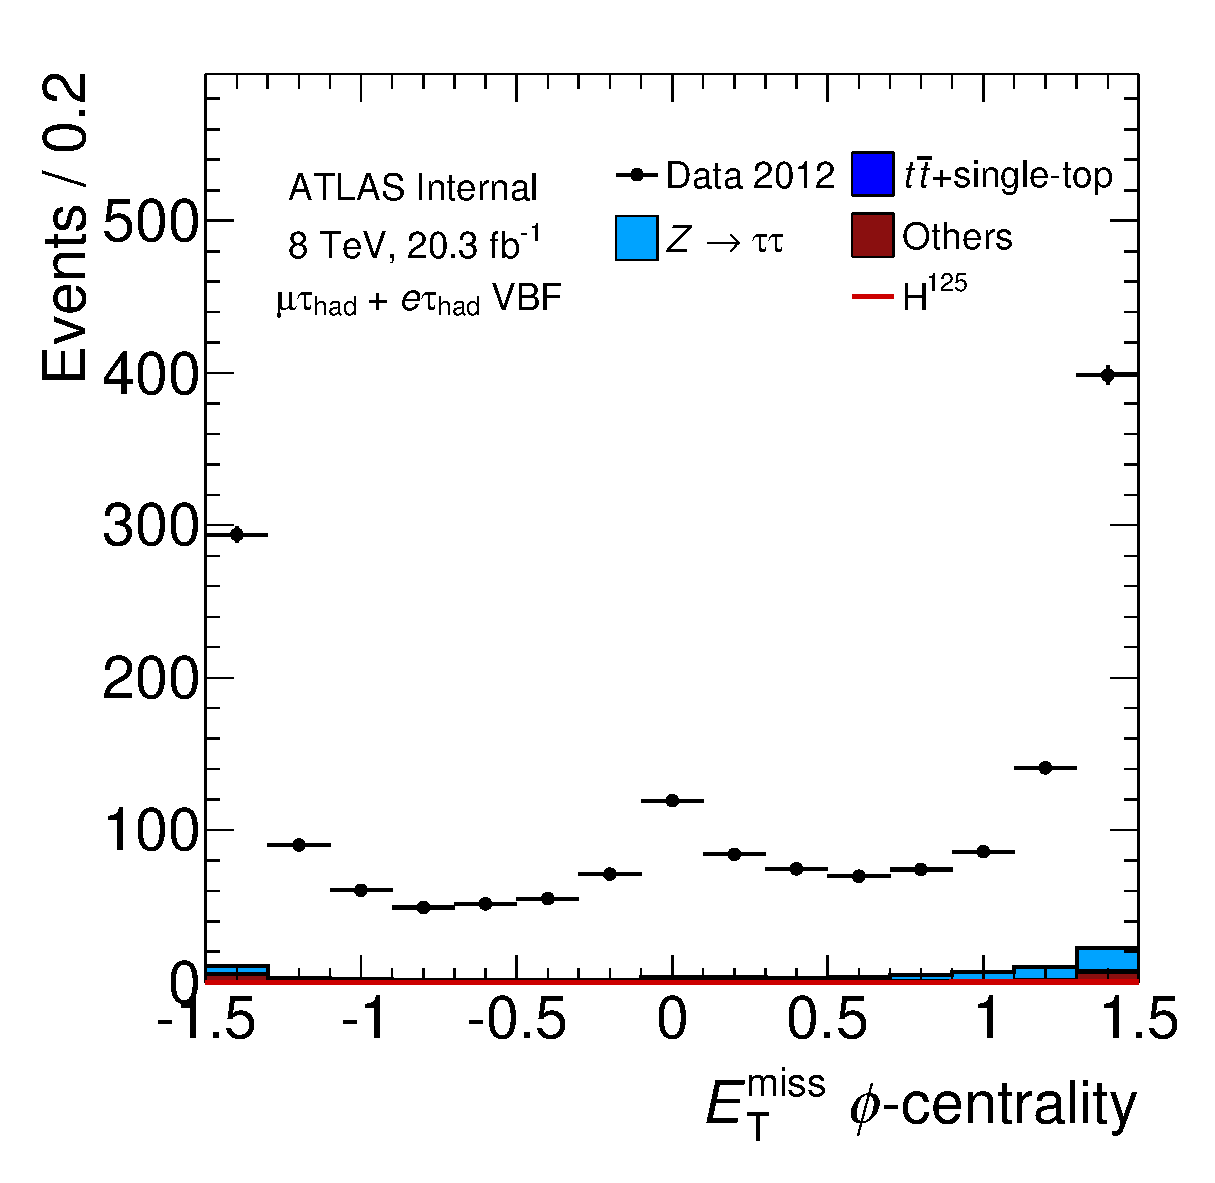
\includegraphics[width=0.32\textwidth]{figures/antitaus/met-phi-centrality}
  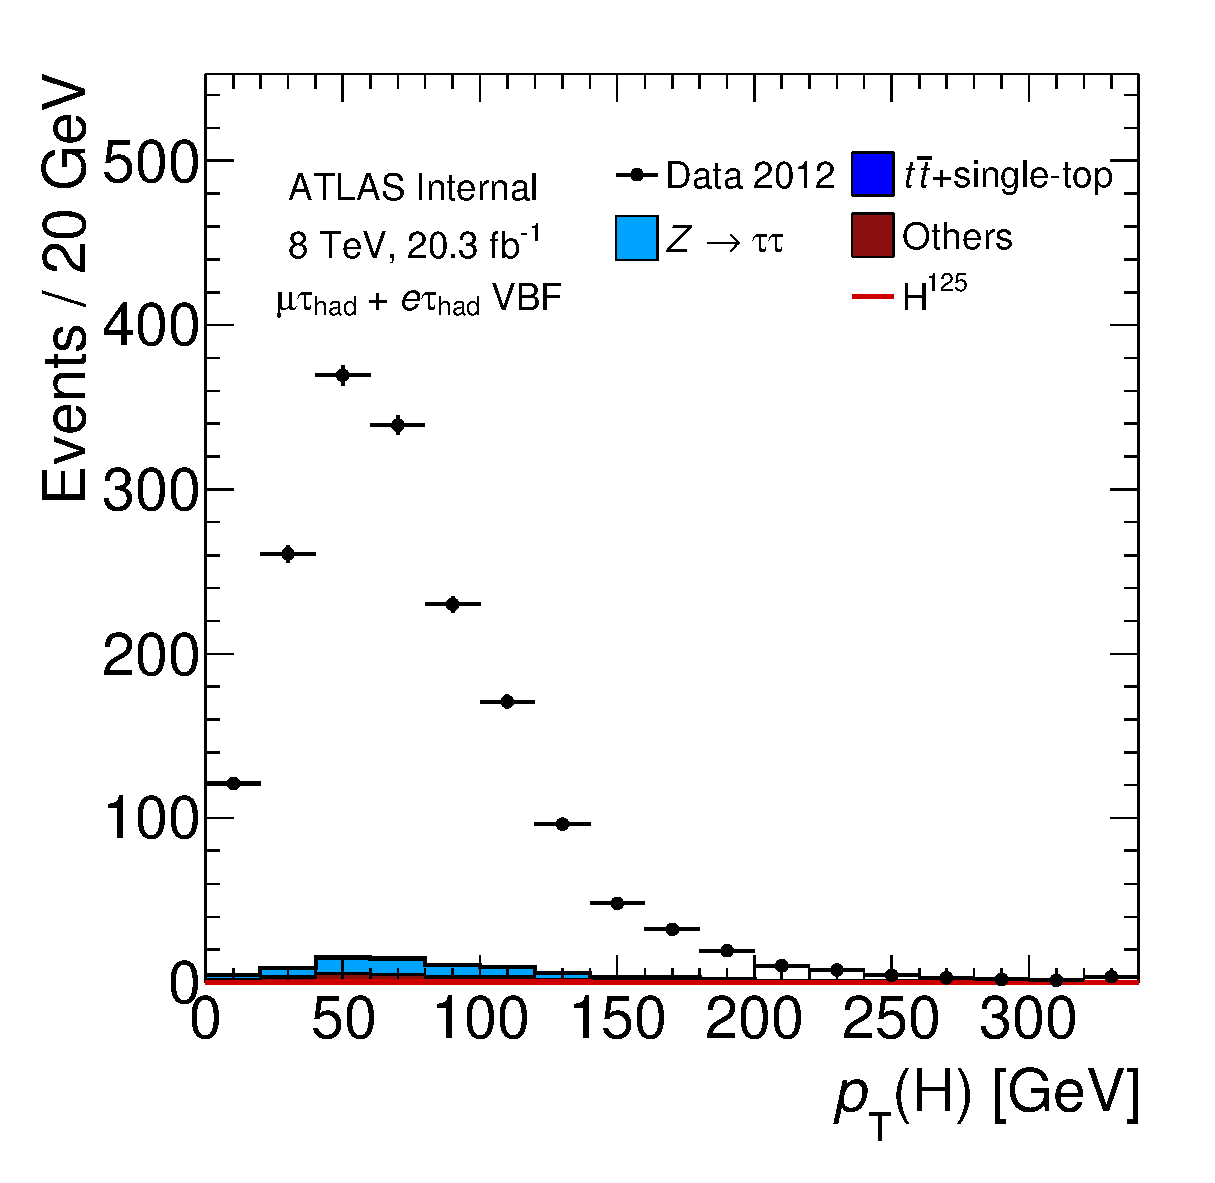
\includegraphics[width=0.32\textwidth]{figures/antitaus/H-pt-hi}
  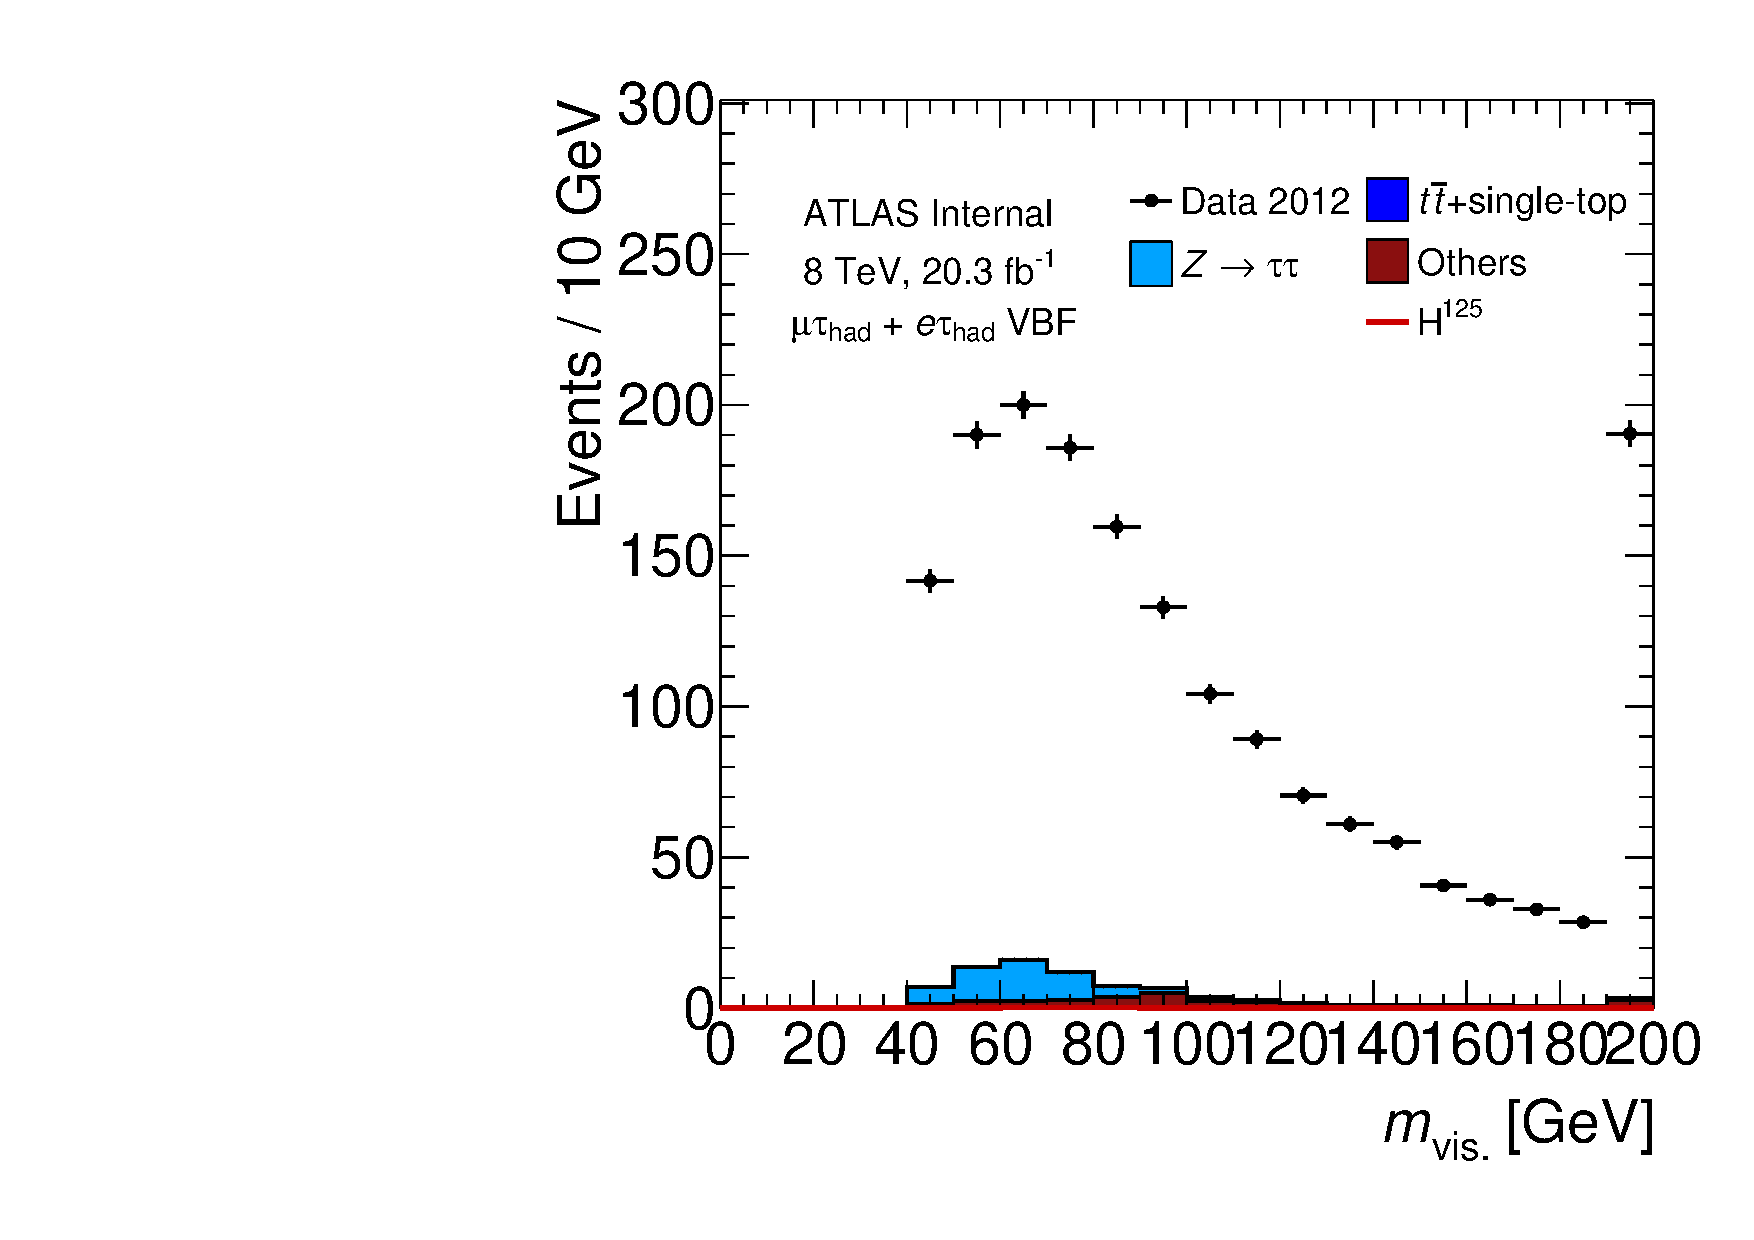
\includegraphics[width=0.32\textwidth]{figures/antitaus/mvis}
  \caption{Data events in the VBF category which fail $\tauh$ identification but fulfill all other requirements. The contamination of $\Ztautaulh$ and other processes without $\fakes$ is less than 10\%.}
  \label{fig:backgrounds-antitaus-taus}
\end{figure}

\clearpage

\begin{figure}[tp]
  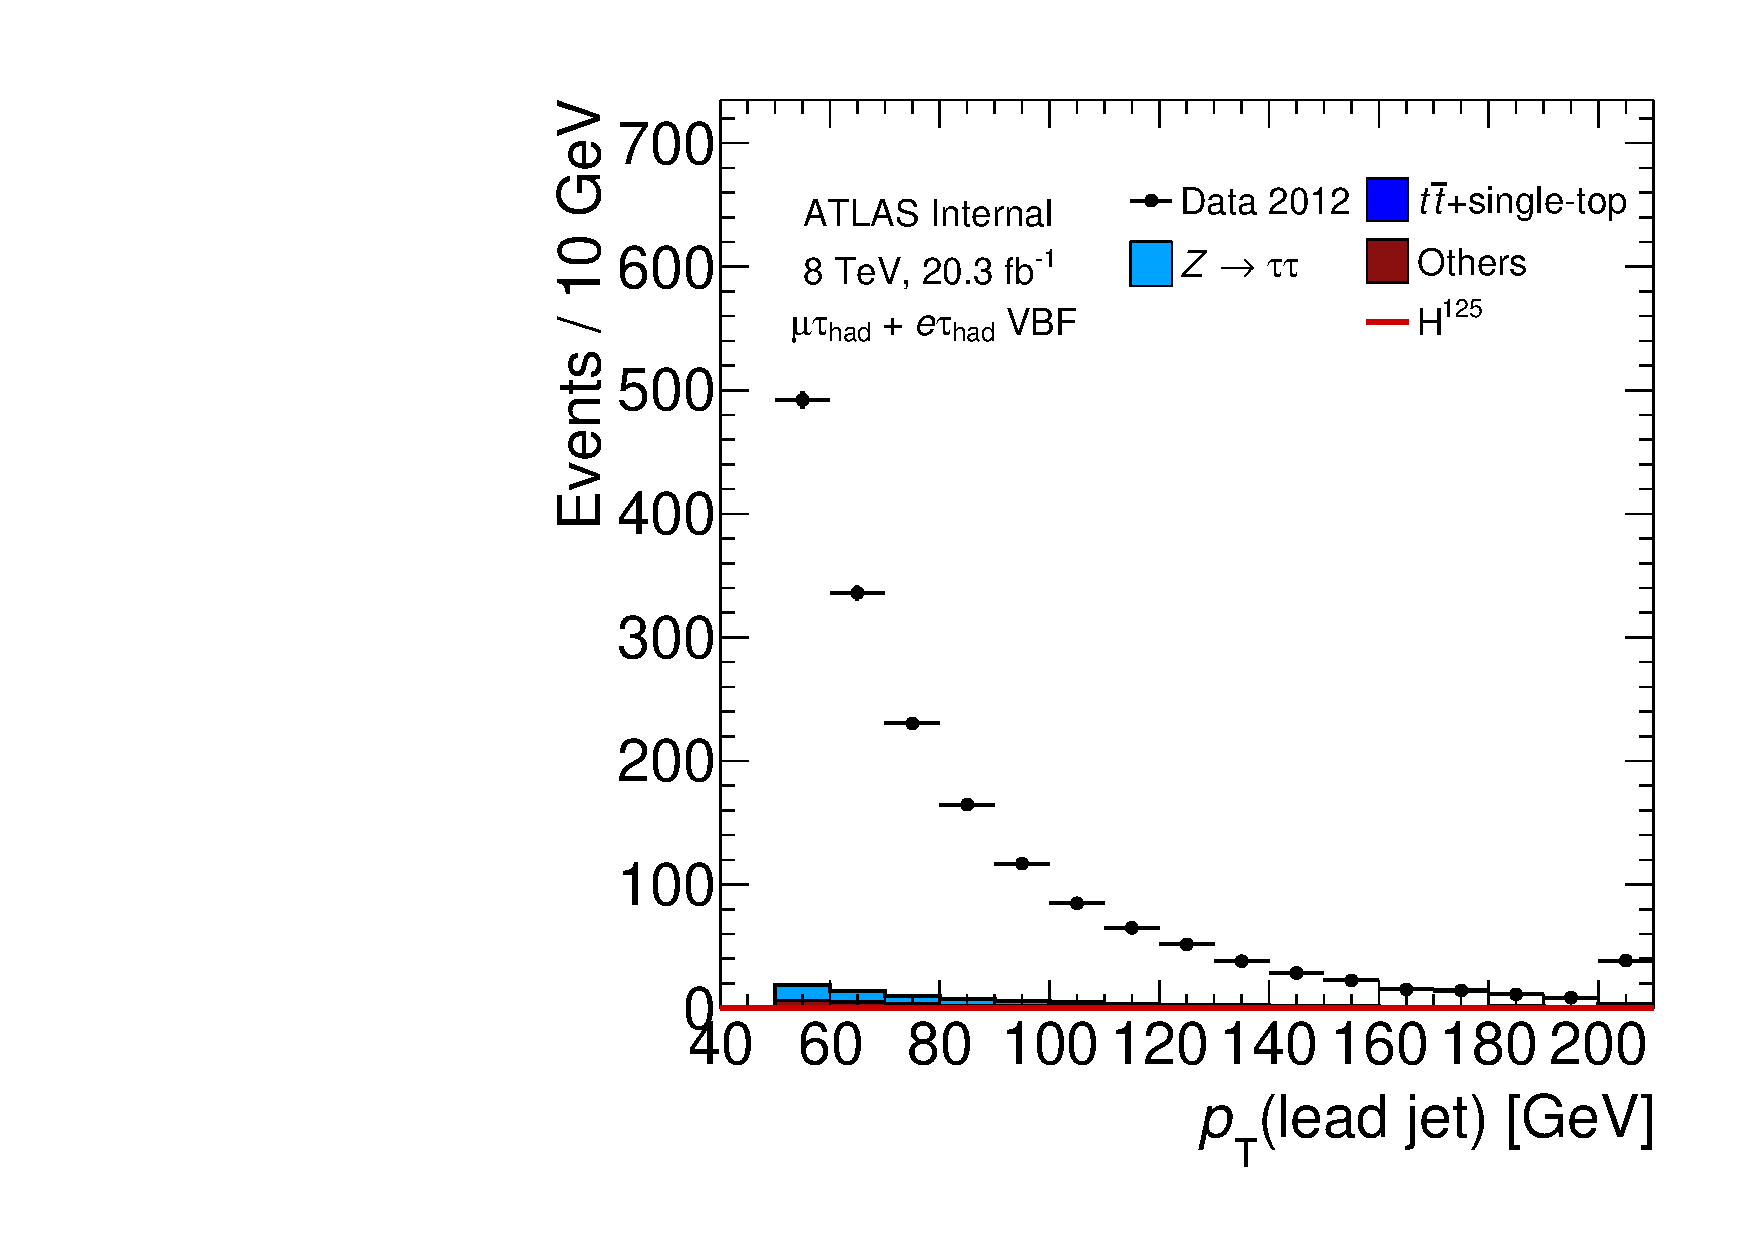
\includegraphics[width=0.32\textwidth]{figures/antitaus/jet-1-pt}
  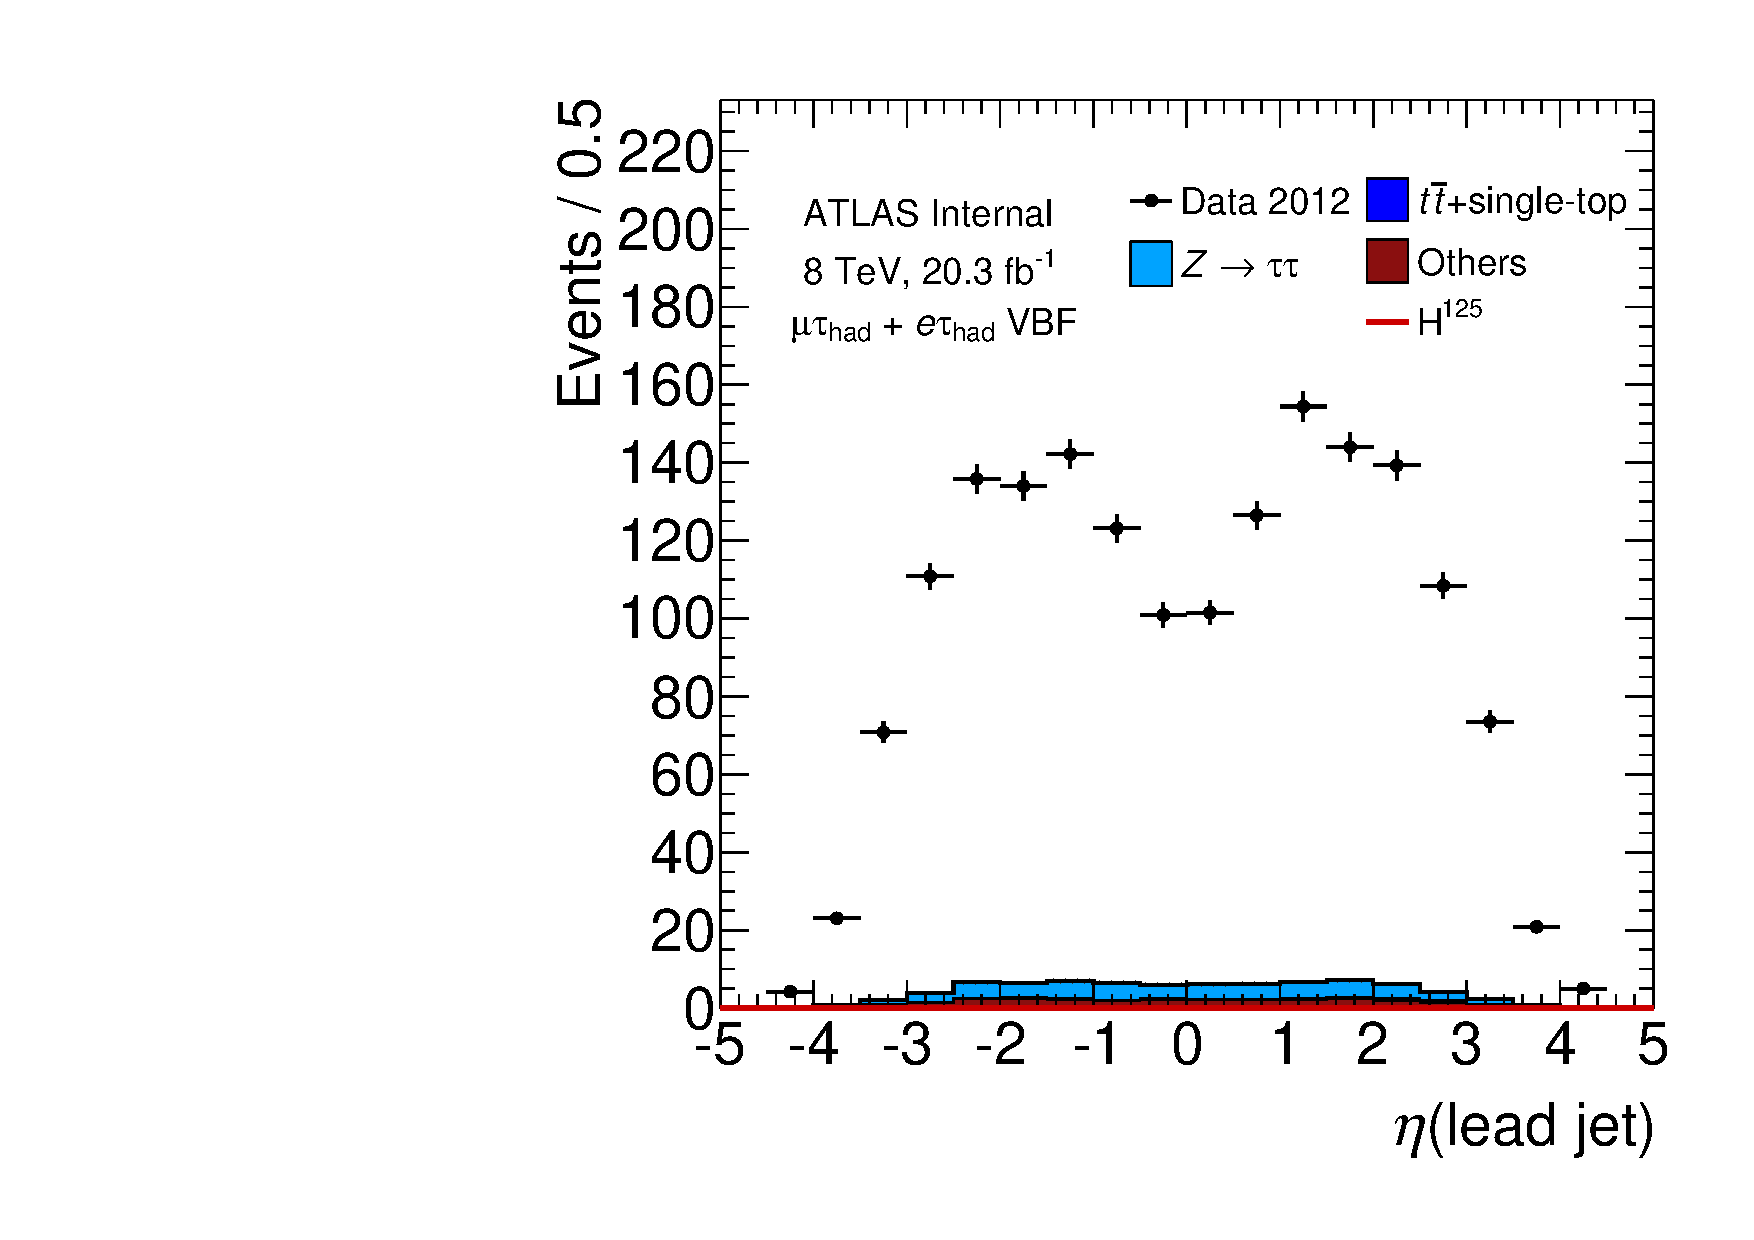
\includegraphics[width=0.32\textwidth]{figures/antitaus/jet-1-eta}
  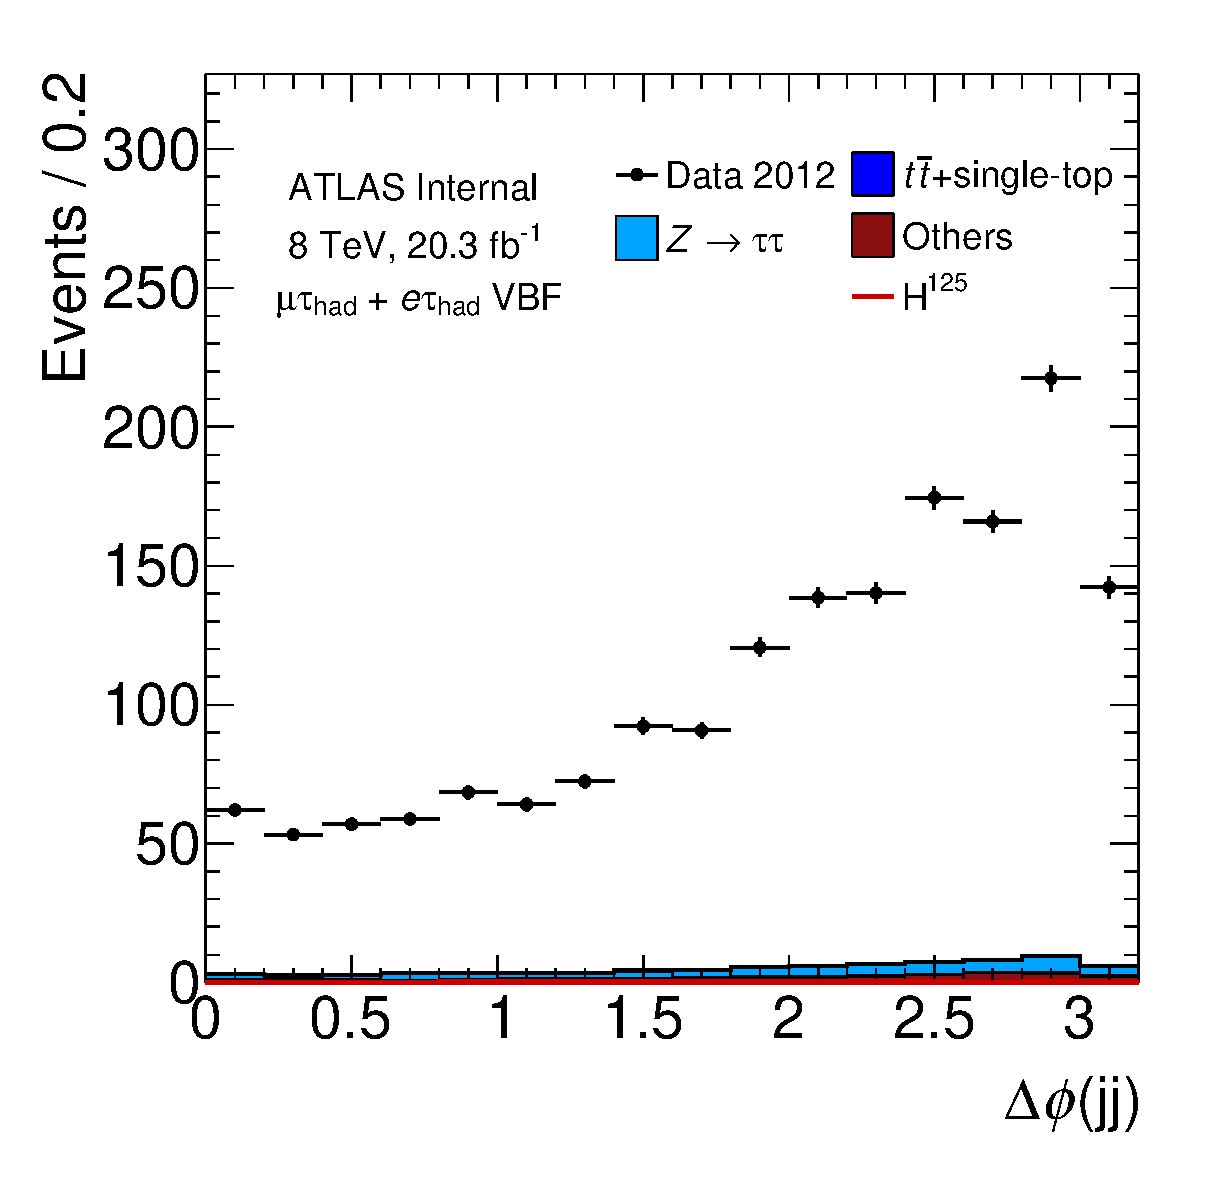
\includegraphics[width=0.32\textwidth]{figures/antitaus/jets-dphi}
  % --------------
  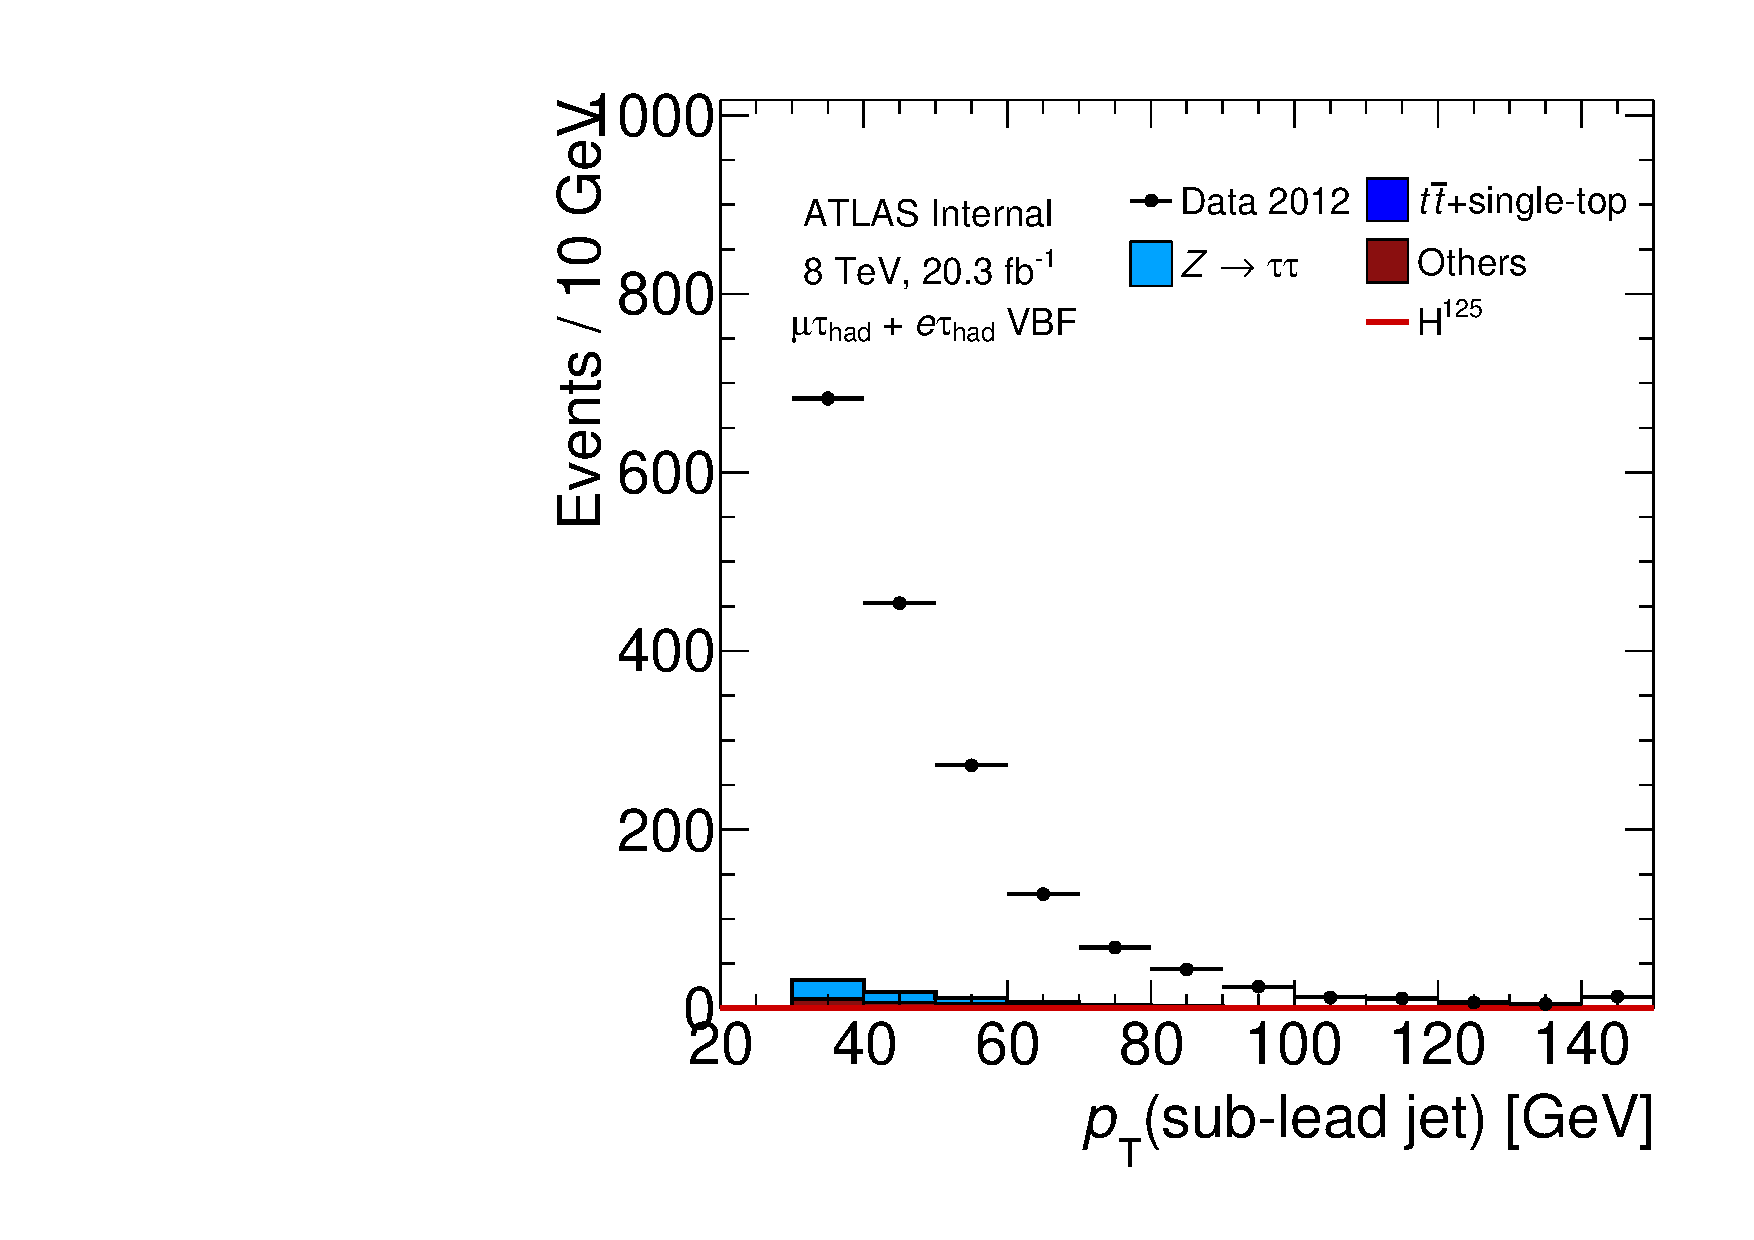
\includegraphics[width=0.32\textwidth]{figures/antitaus/jet-2-pt}
  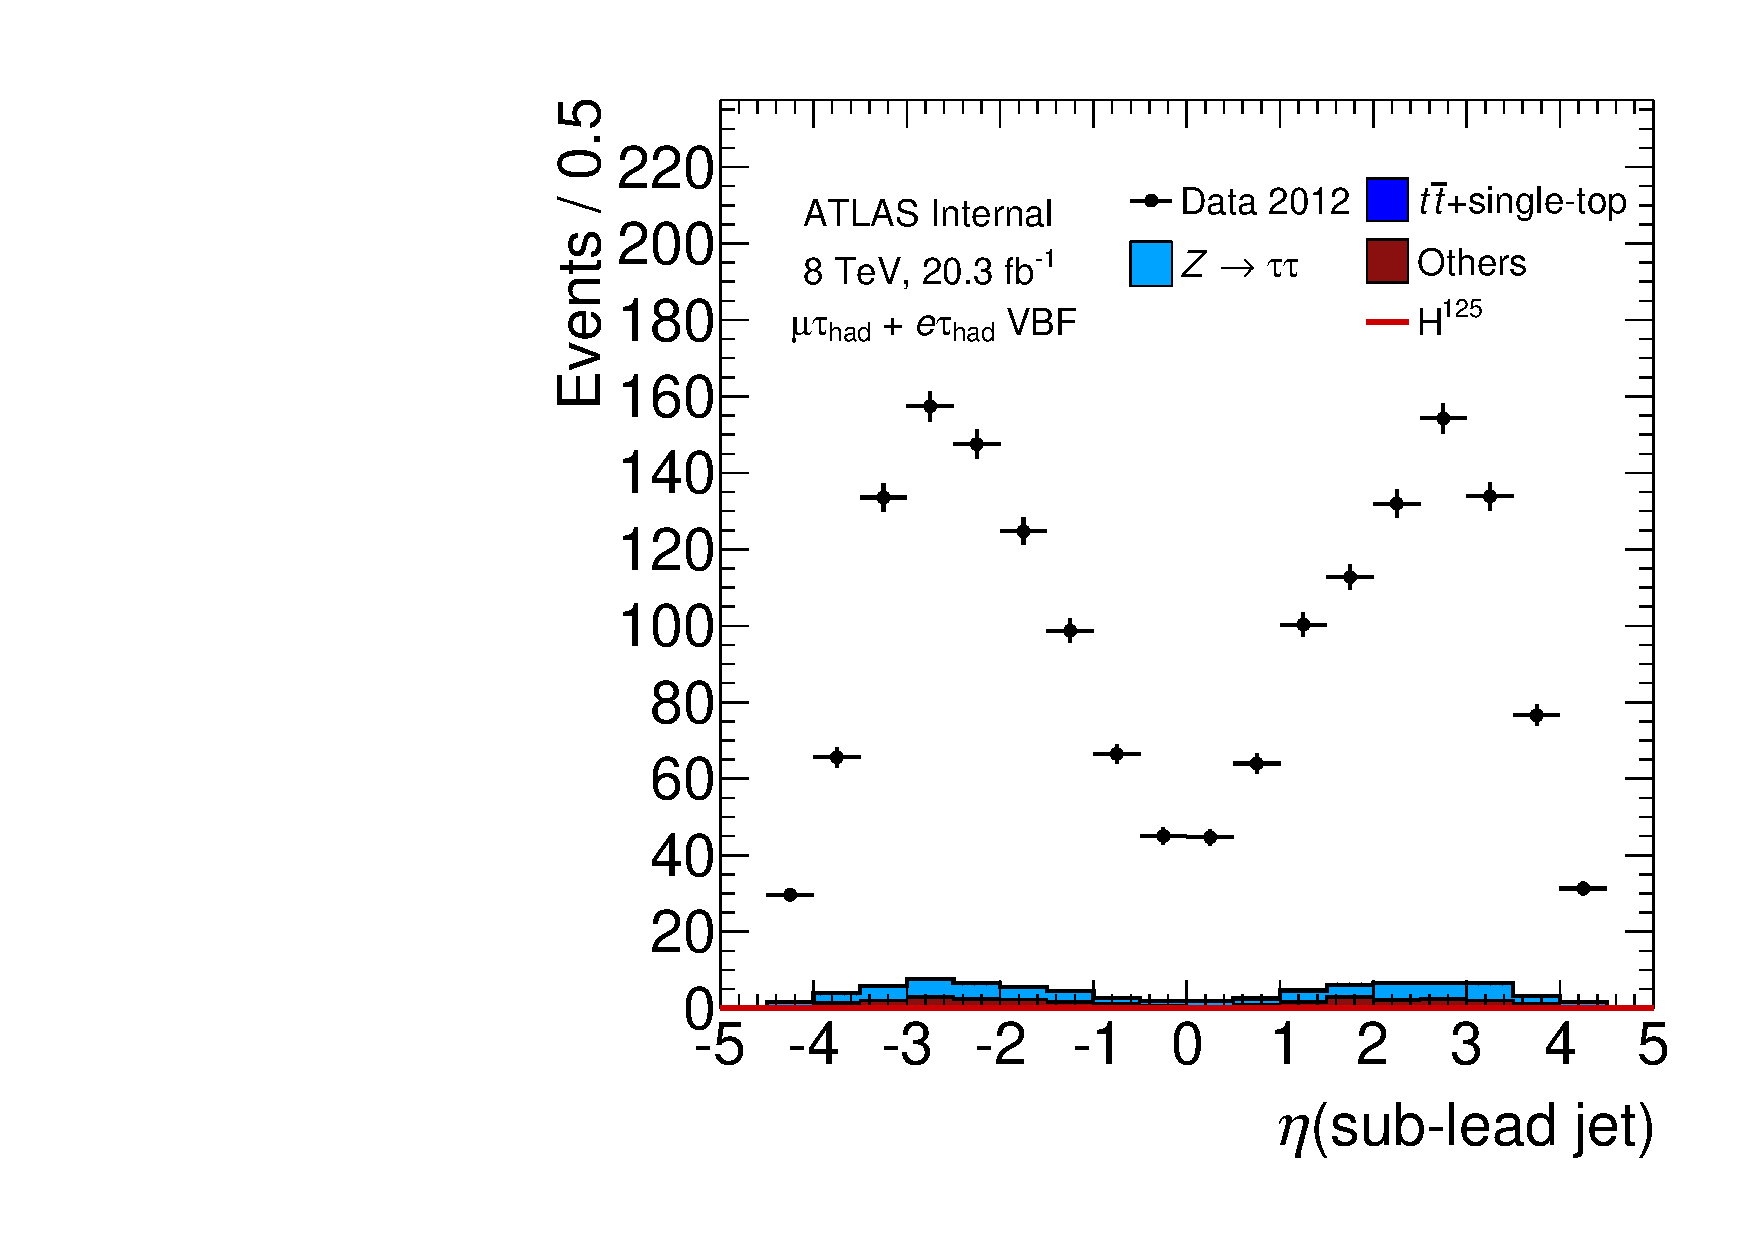
\includegraphics[width=0.32\textwidth]{figures/antitaus/jet-2-eta}
  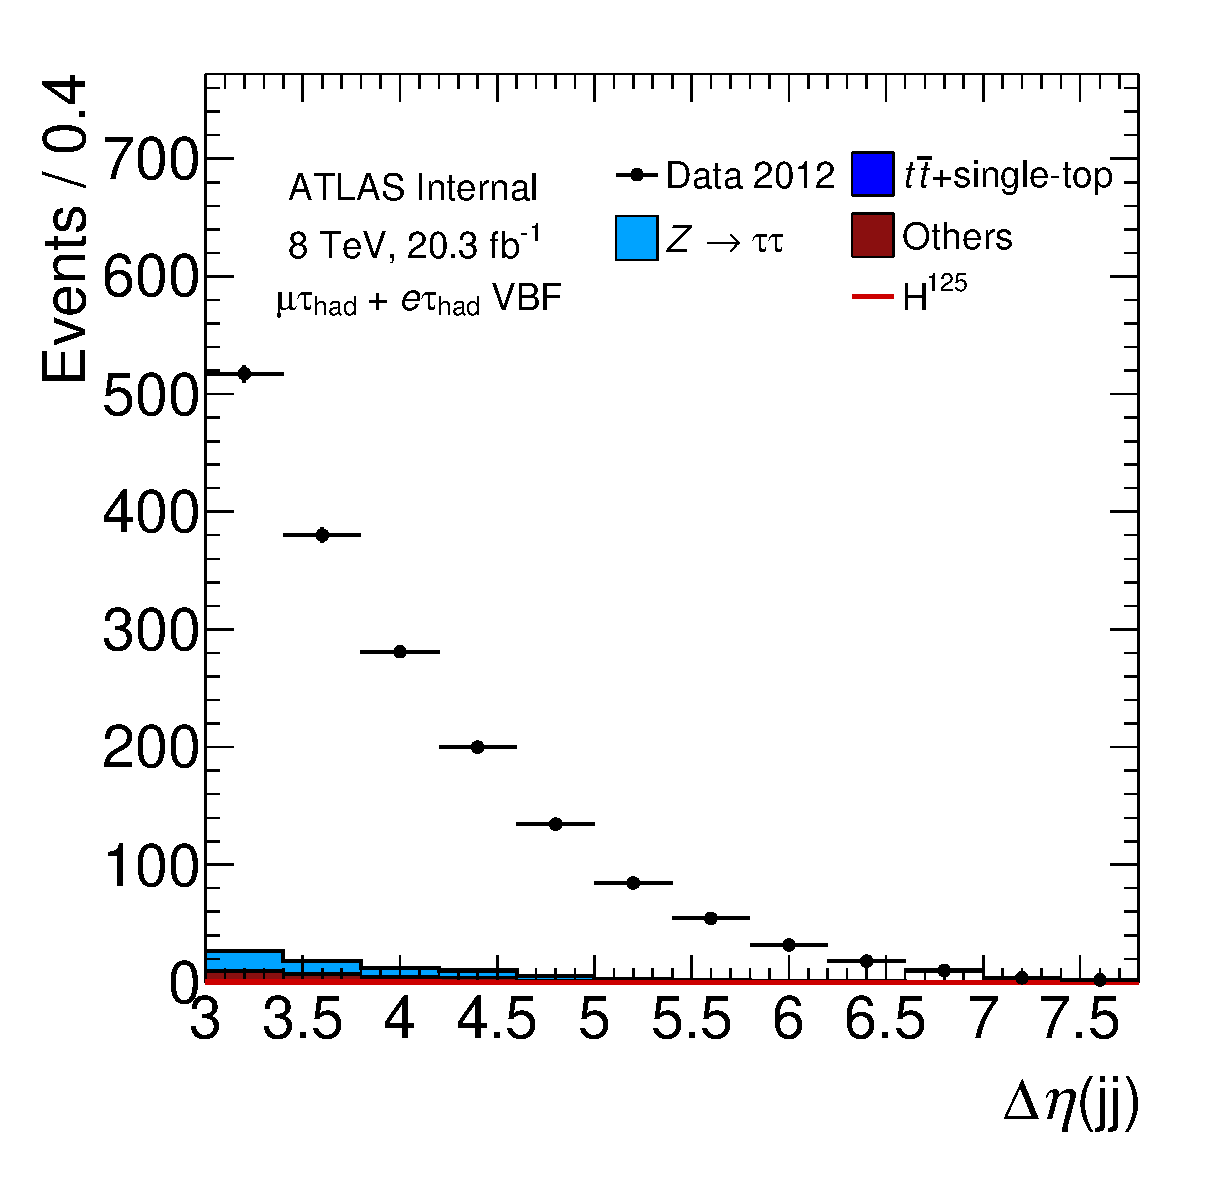
\includegraphics[width=0.32\textwidth]{figures/antitaus/jets-deta}
  % --------------
  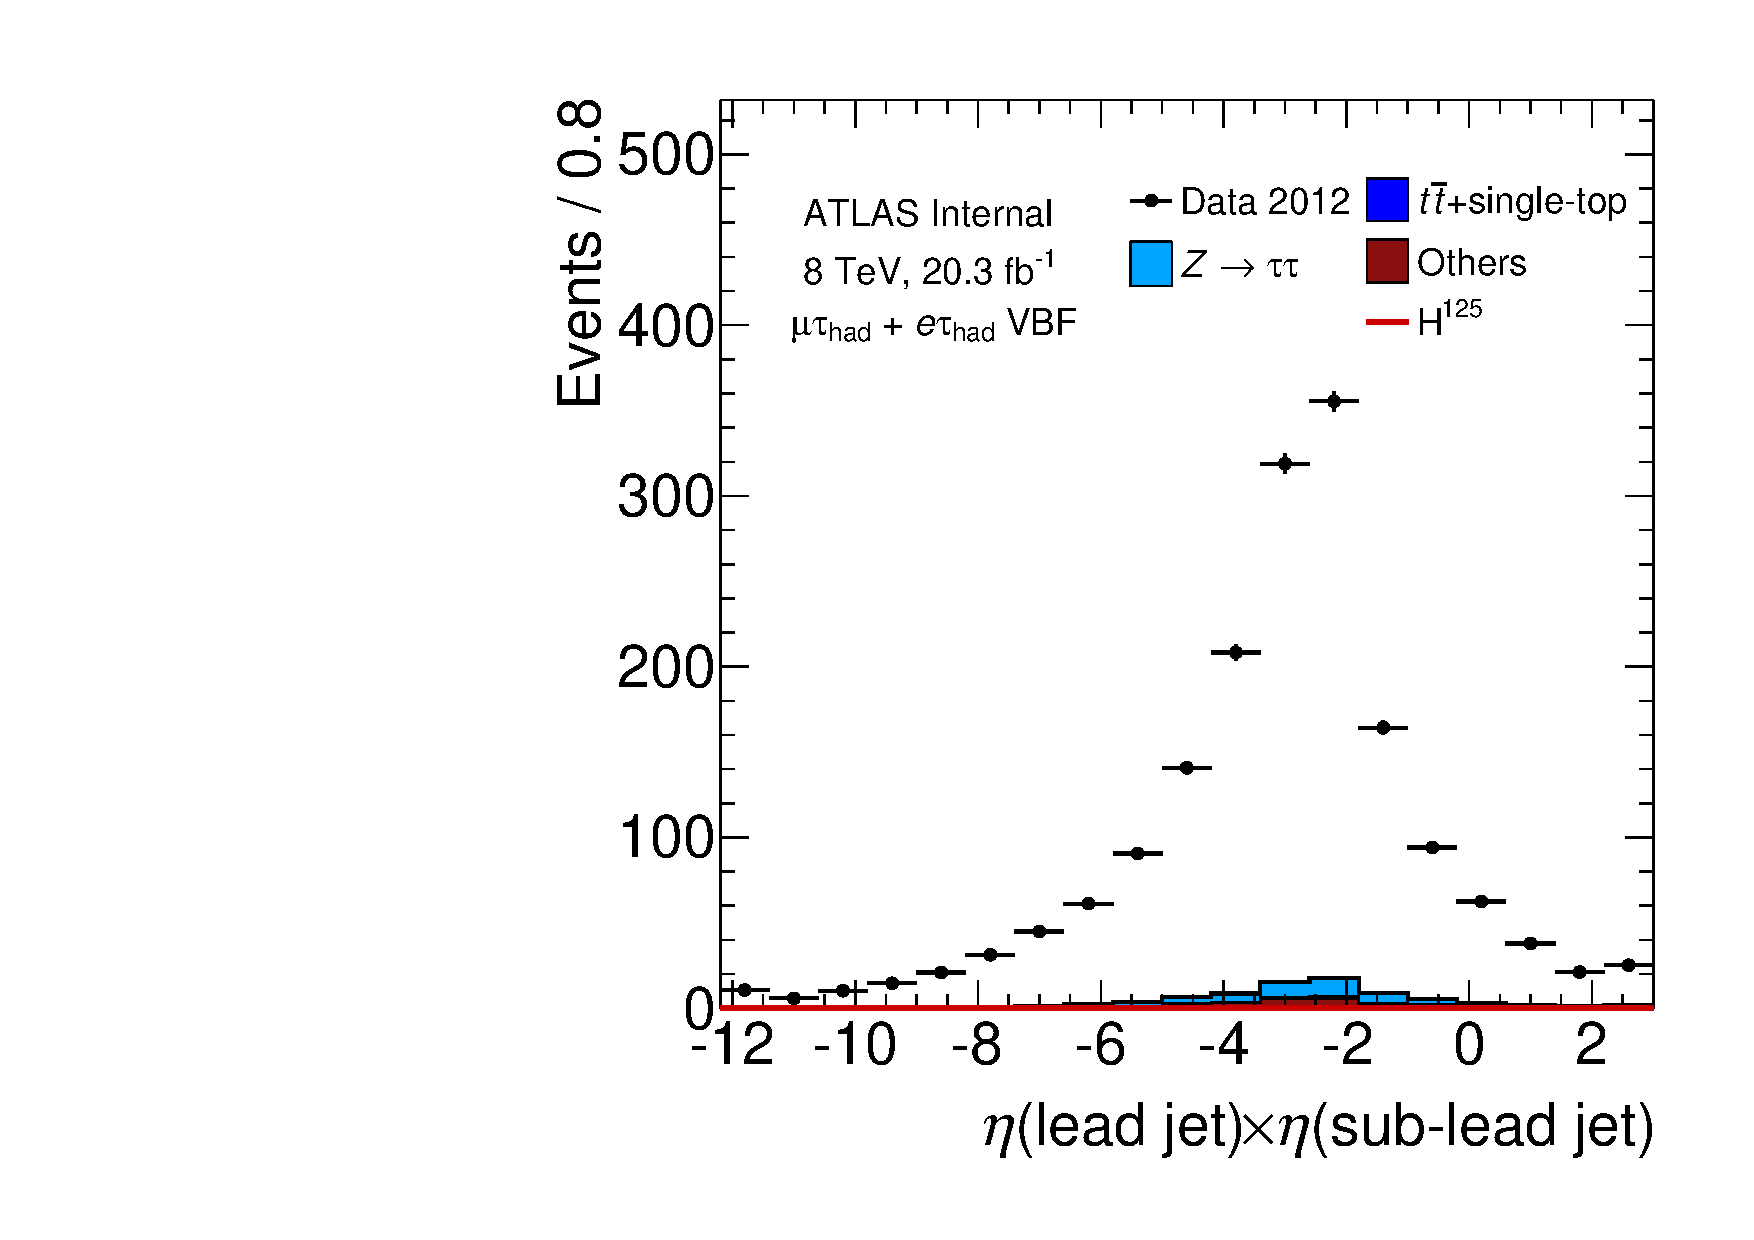
\includegraphics[width=0.32\textwidth]{figures/antitaus/jets-etaprod}
  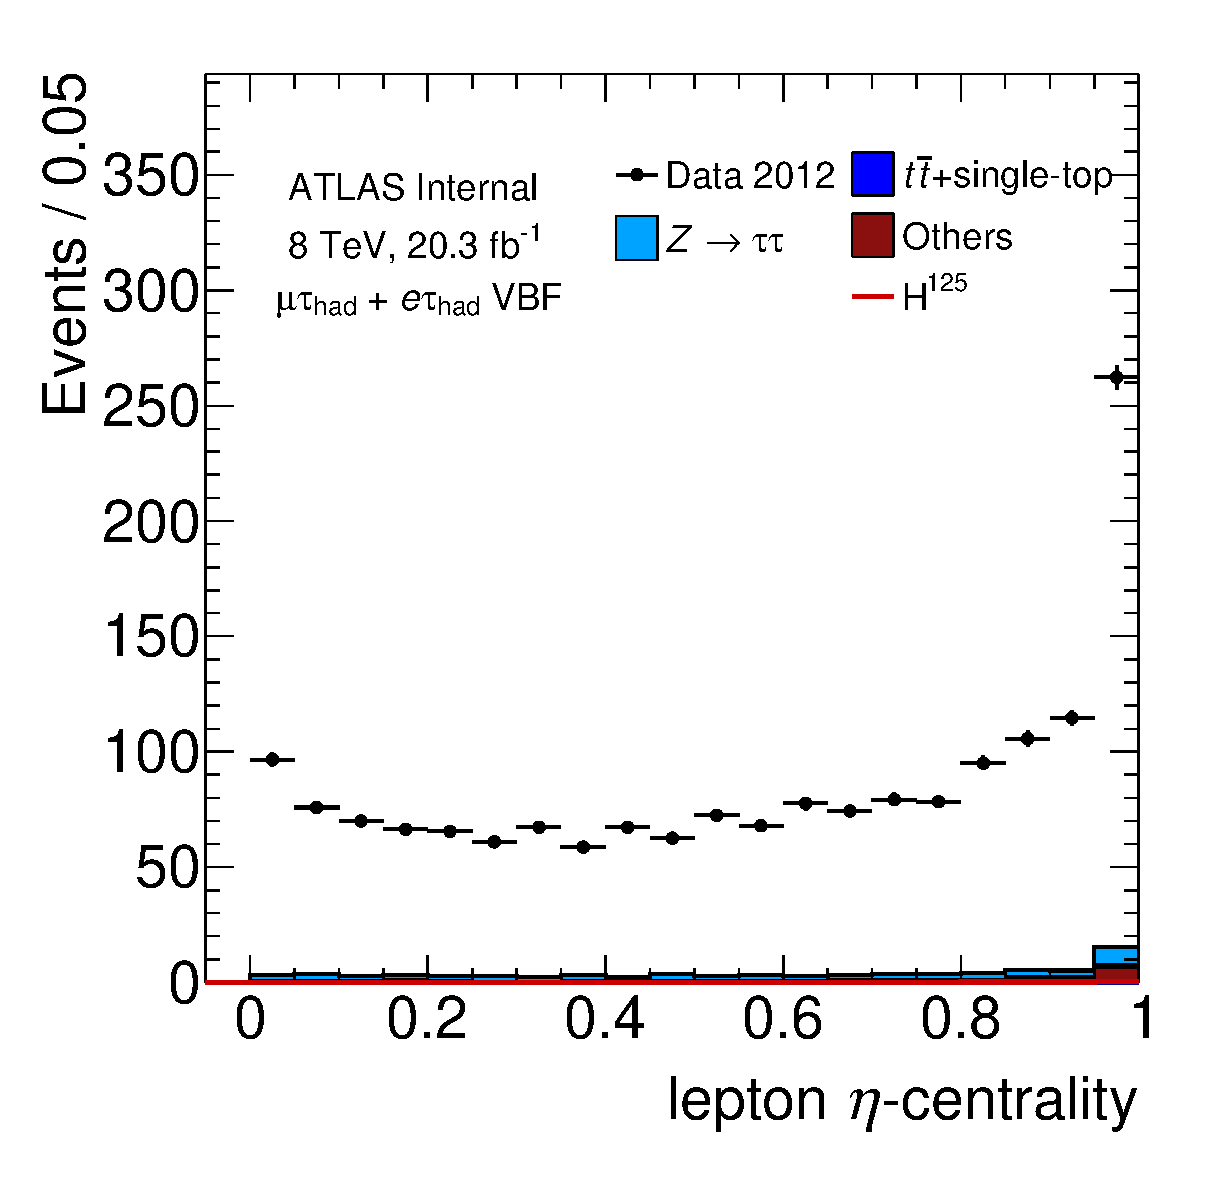
\includegraphics[width=0.32\textwidth]{figures/antitaus/lep-eta-centrality}
  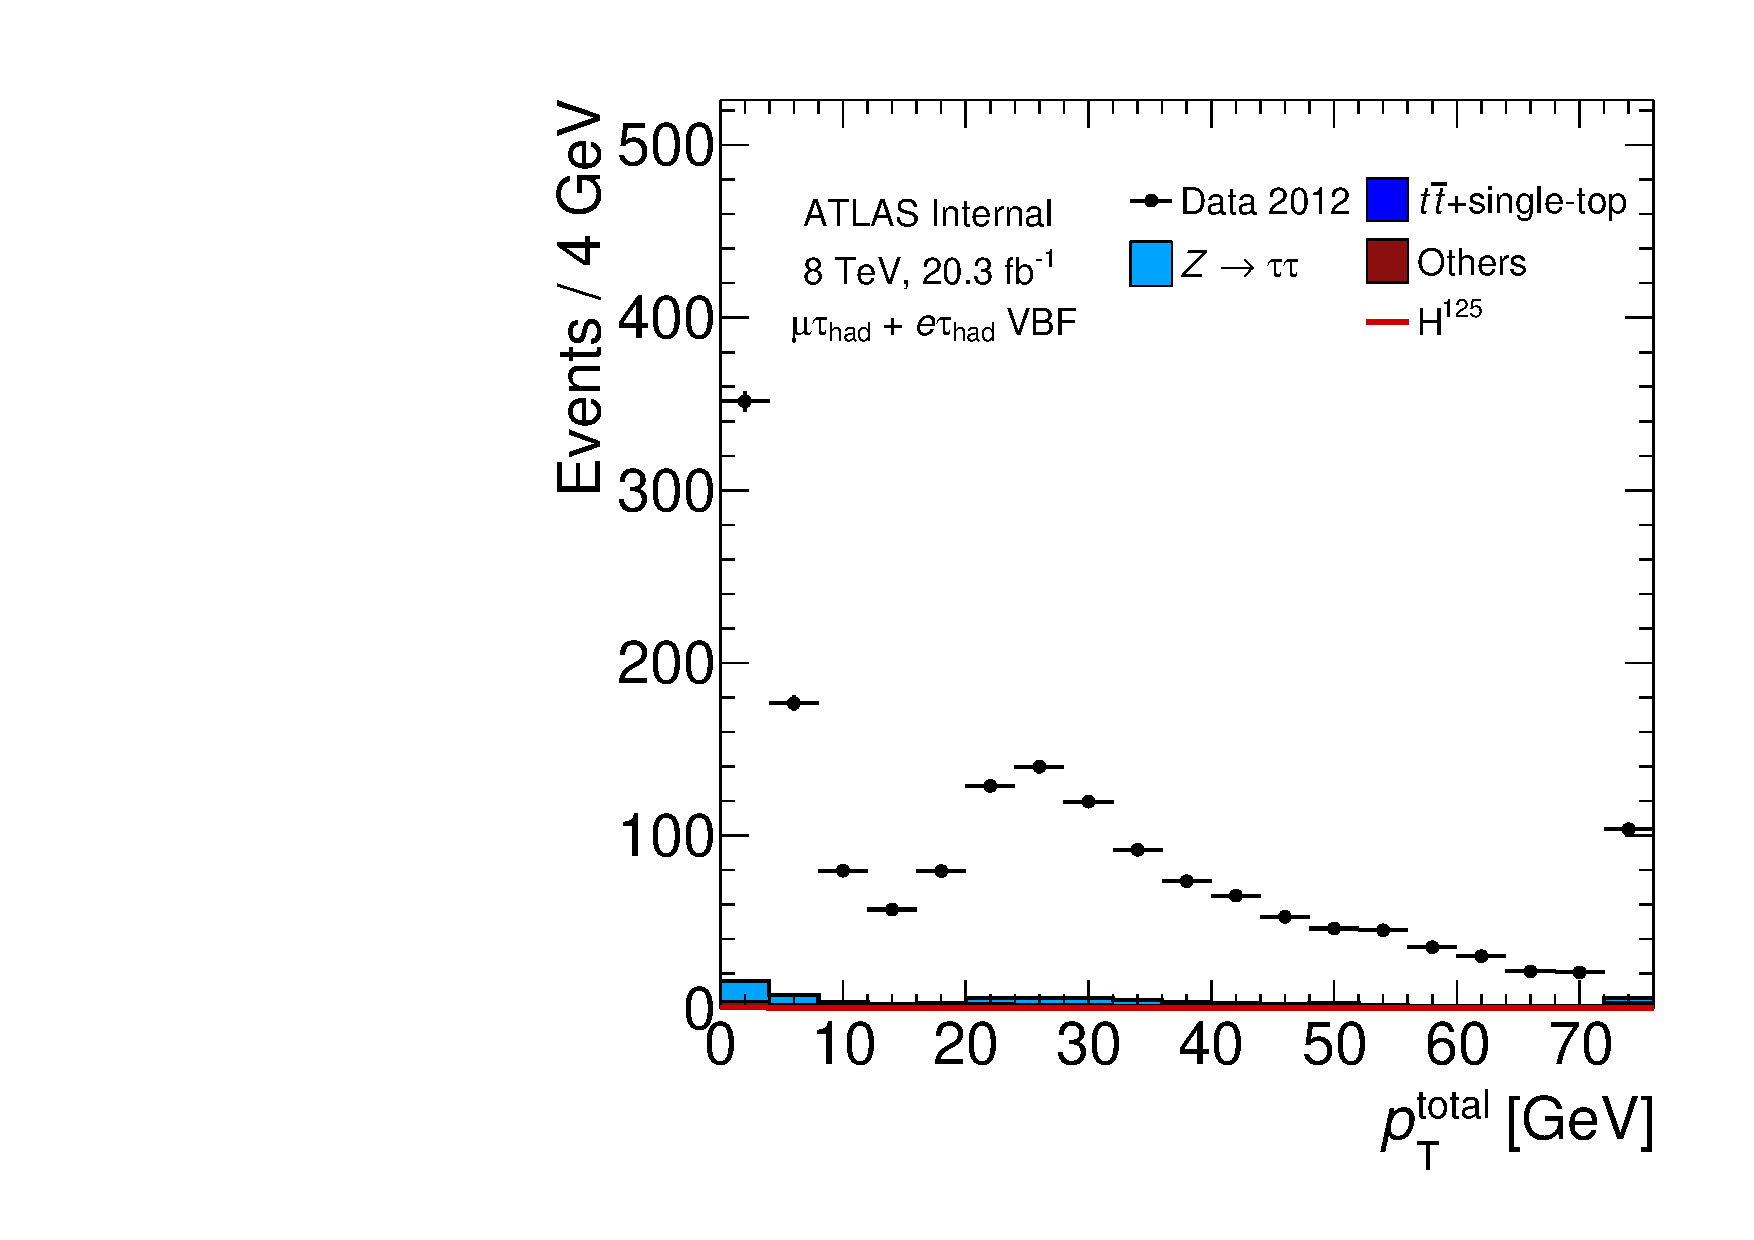
\includegraphics[width=0.32\textwidth]{figures/antitaus/system-pt}
  % --------------
  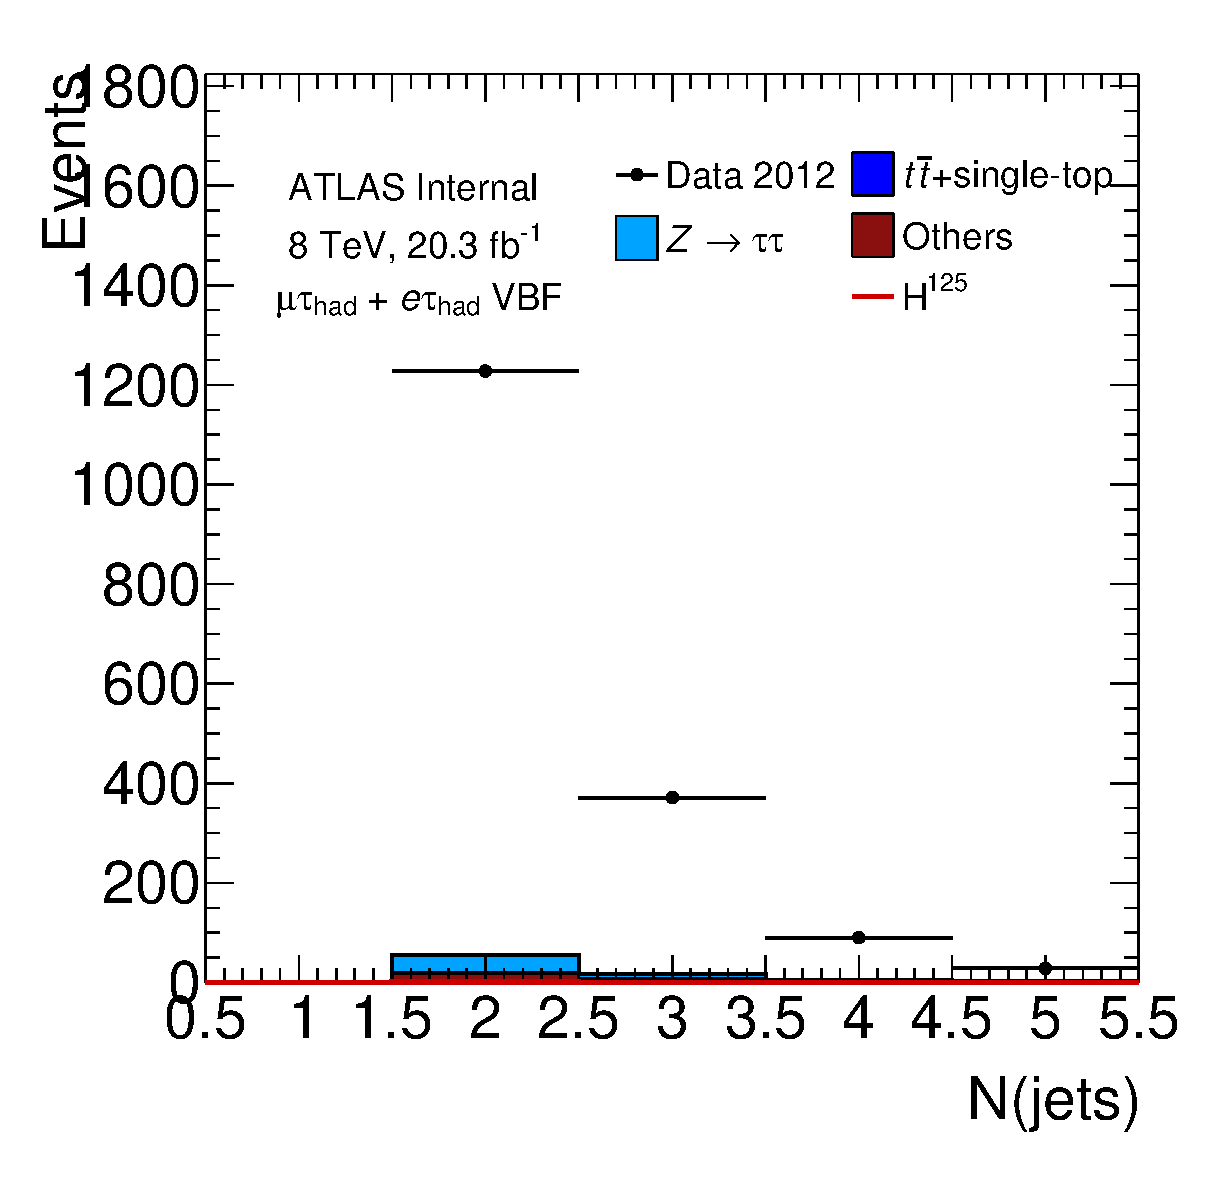
\includegraphics[width=0.32\textwidth]{figures/antitaus/n-jets30}
  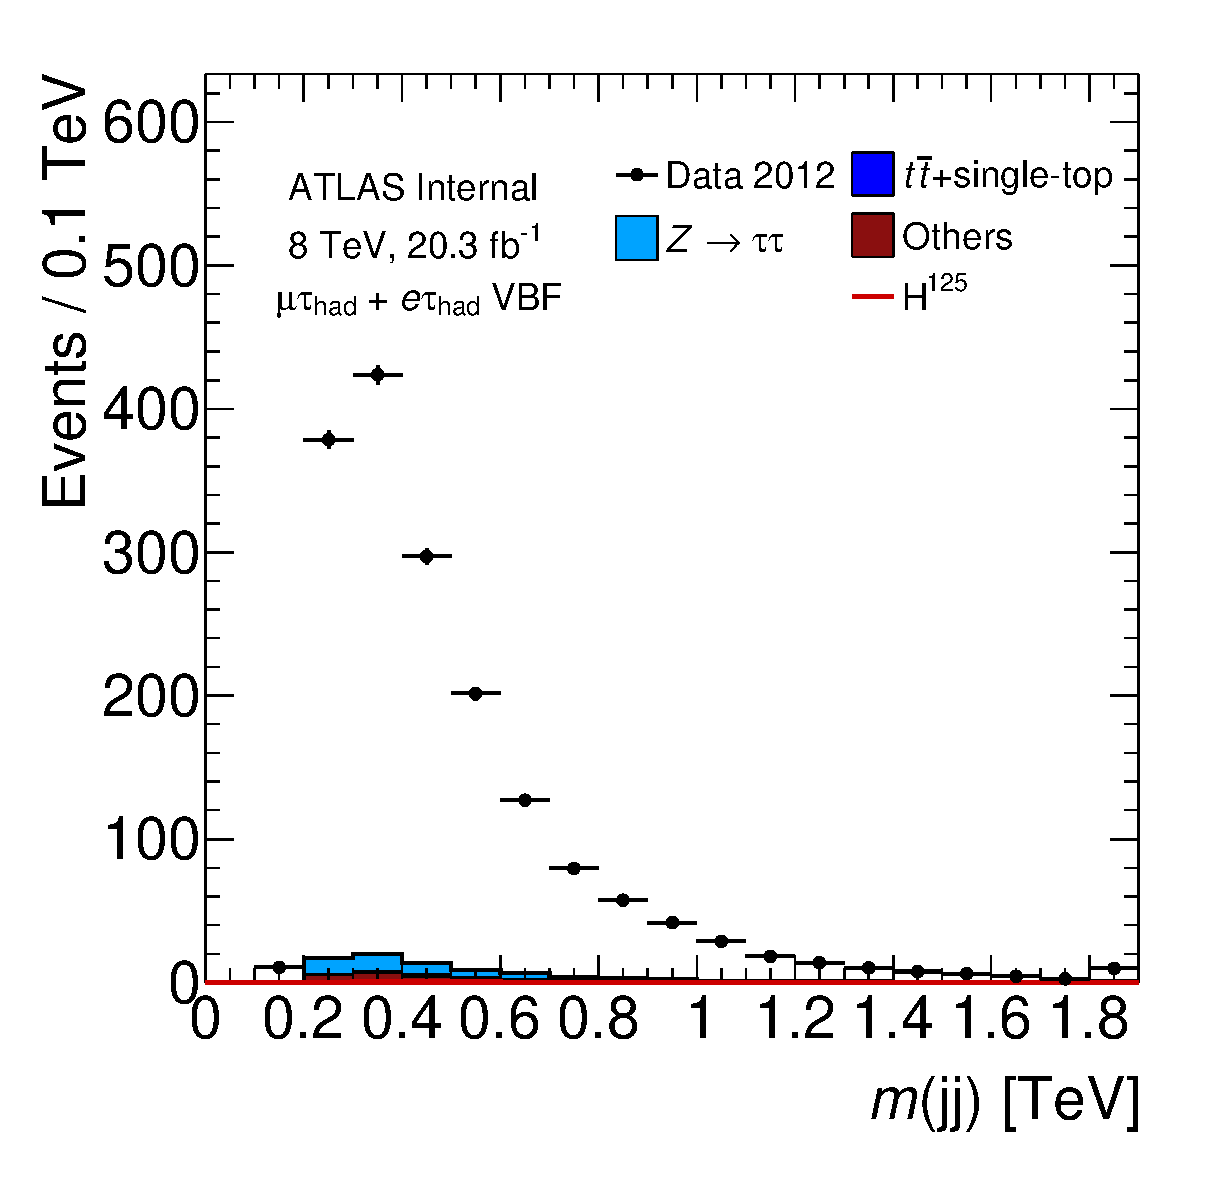
\includegraphics[width=0.32\textwidth]{figures/antitaus/dijet-m-veryhigh}
  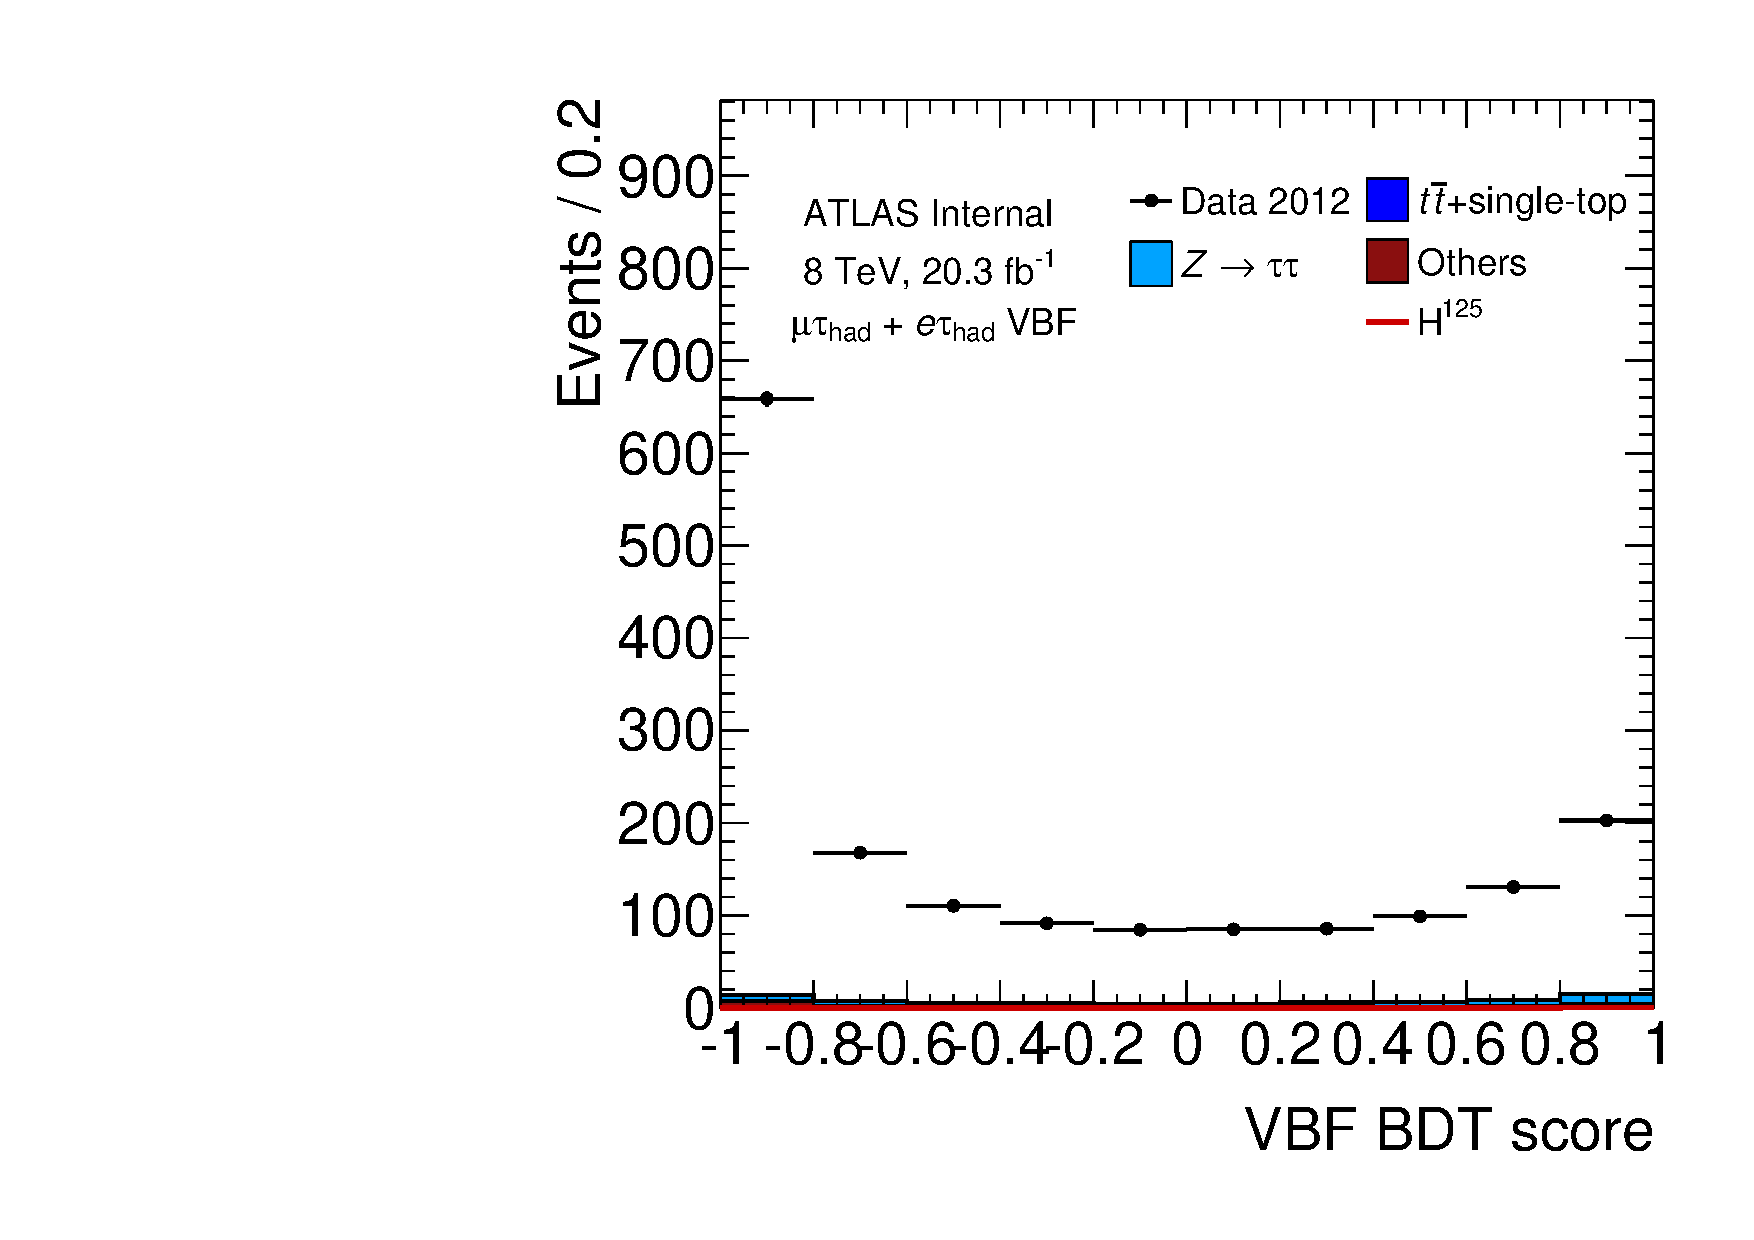
\includegraphics[width=0.32\textwidth]{figures/antitaus/BDTEve-VBF}
  \caption{Data events in the VBF category which fail $\tauh$ identification but fulfill all other requirements. The contamination of $\Ztautaulh$ and other processes without $\fakes$ is less than 10\%.}
  \label{fig:backgrounds-antitaus-jets}
\end{figure}

\clearpage

\begin{figure}[tp]
  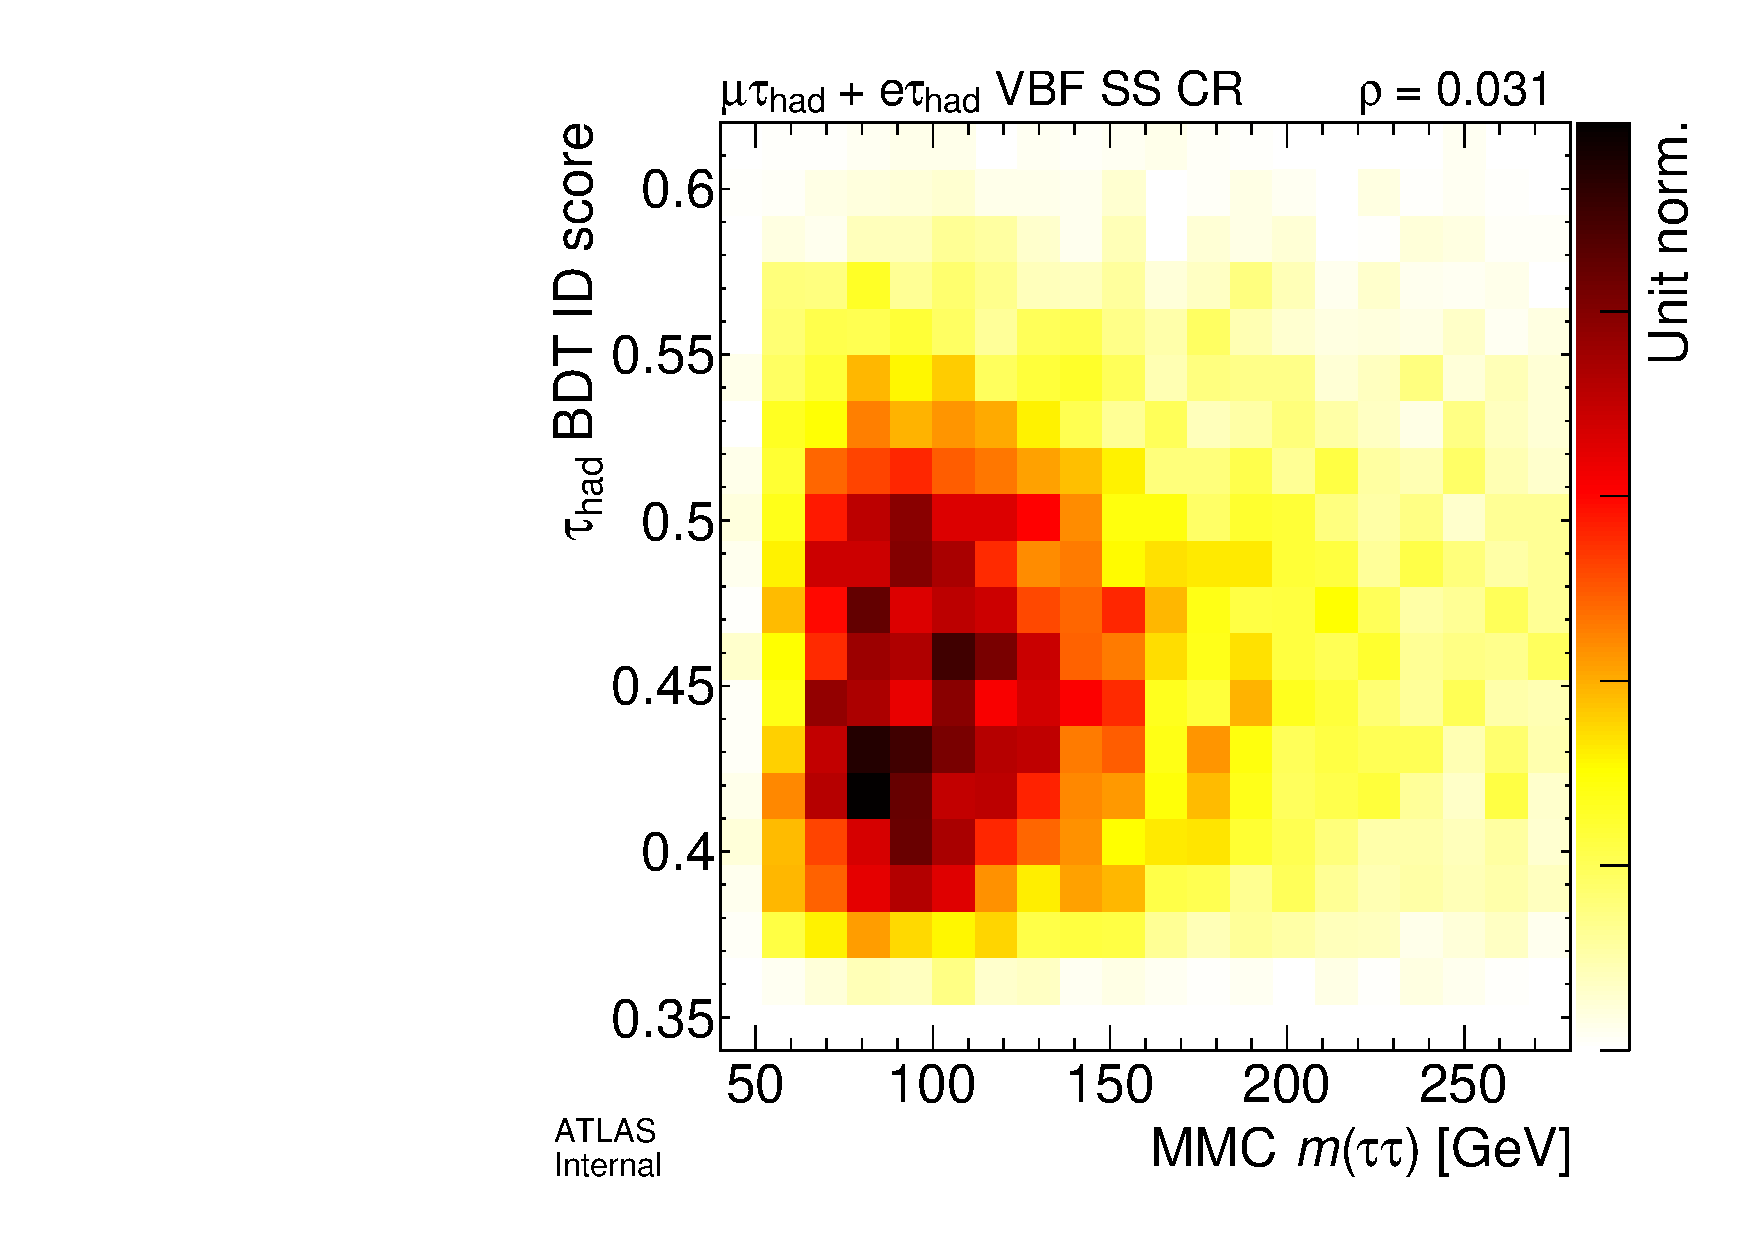
\includegraphics[width=0.32\textwidth]{figures/tauidcorrelations/tauid_vs_mMMC}
  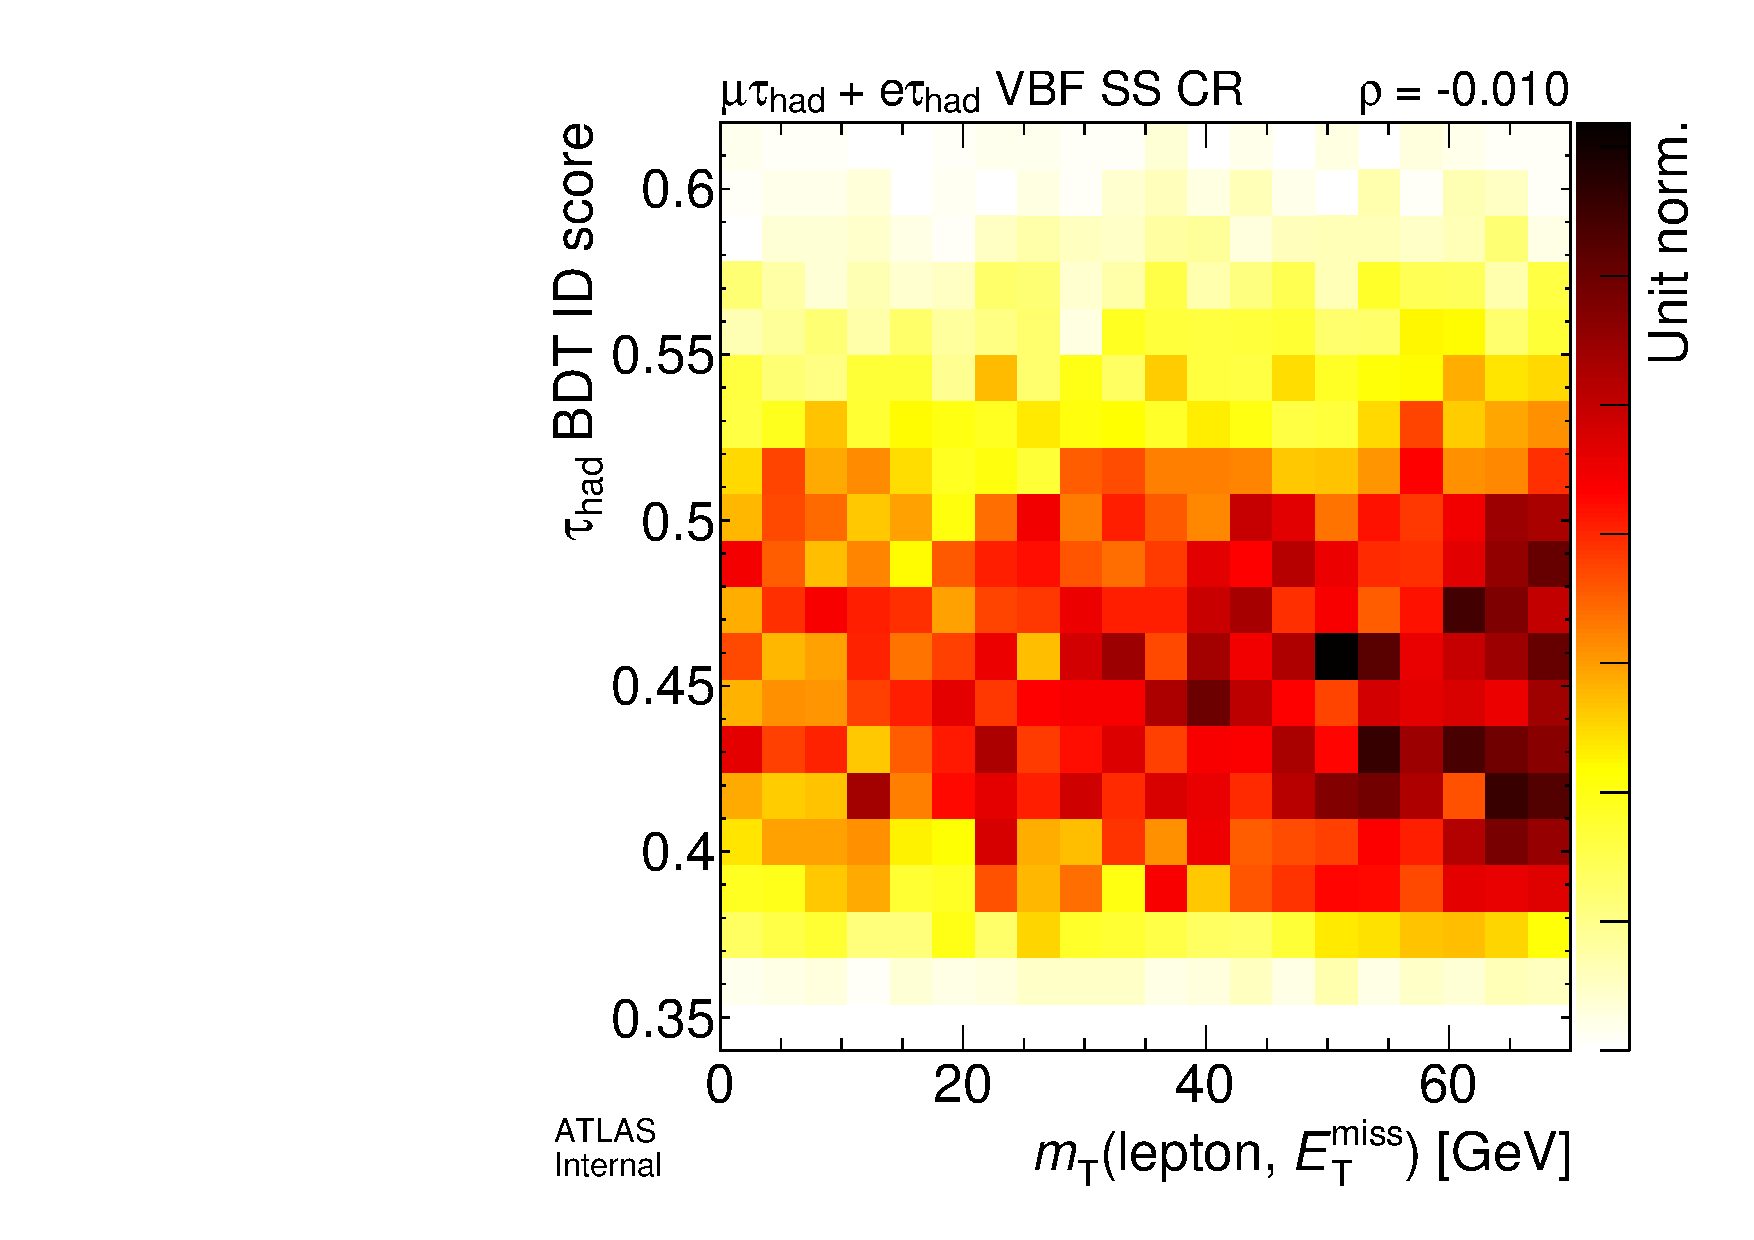
\includegraphics[width=0.32\textwidth]{figures/tauidcorrelations/tauid_vs_mT}
  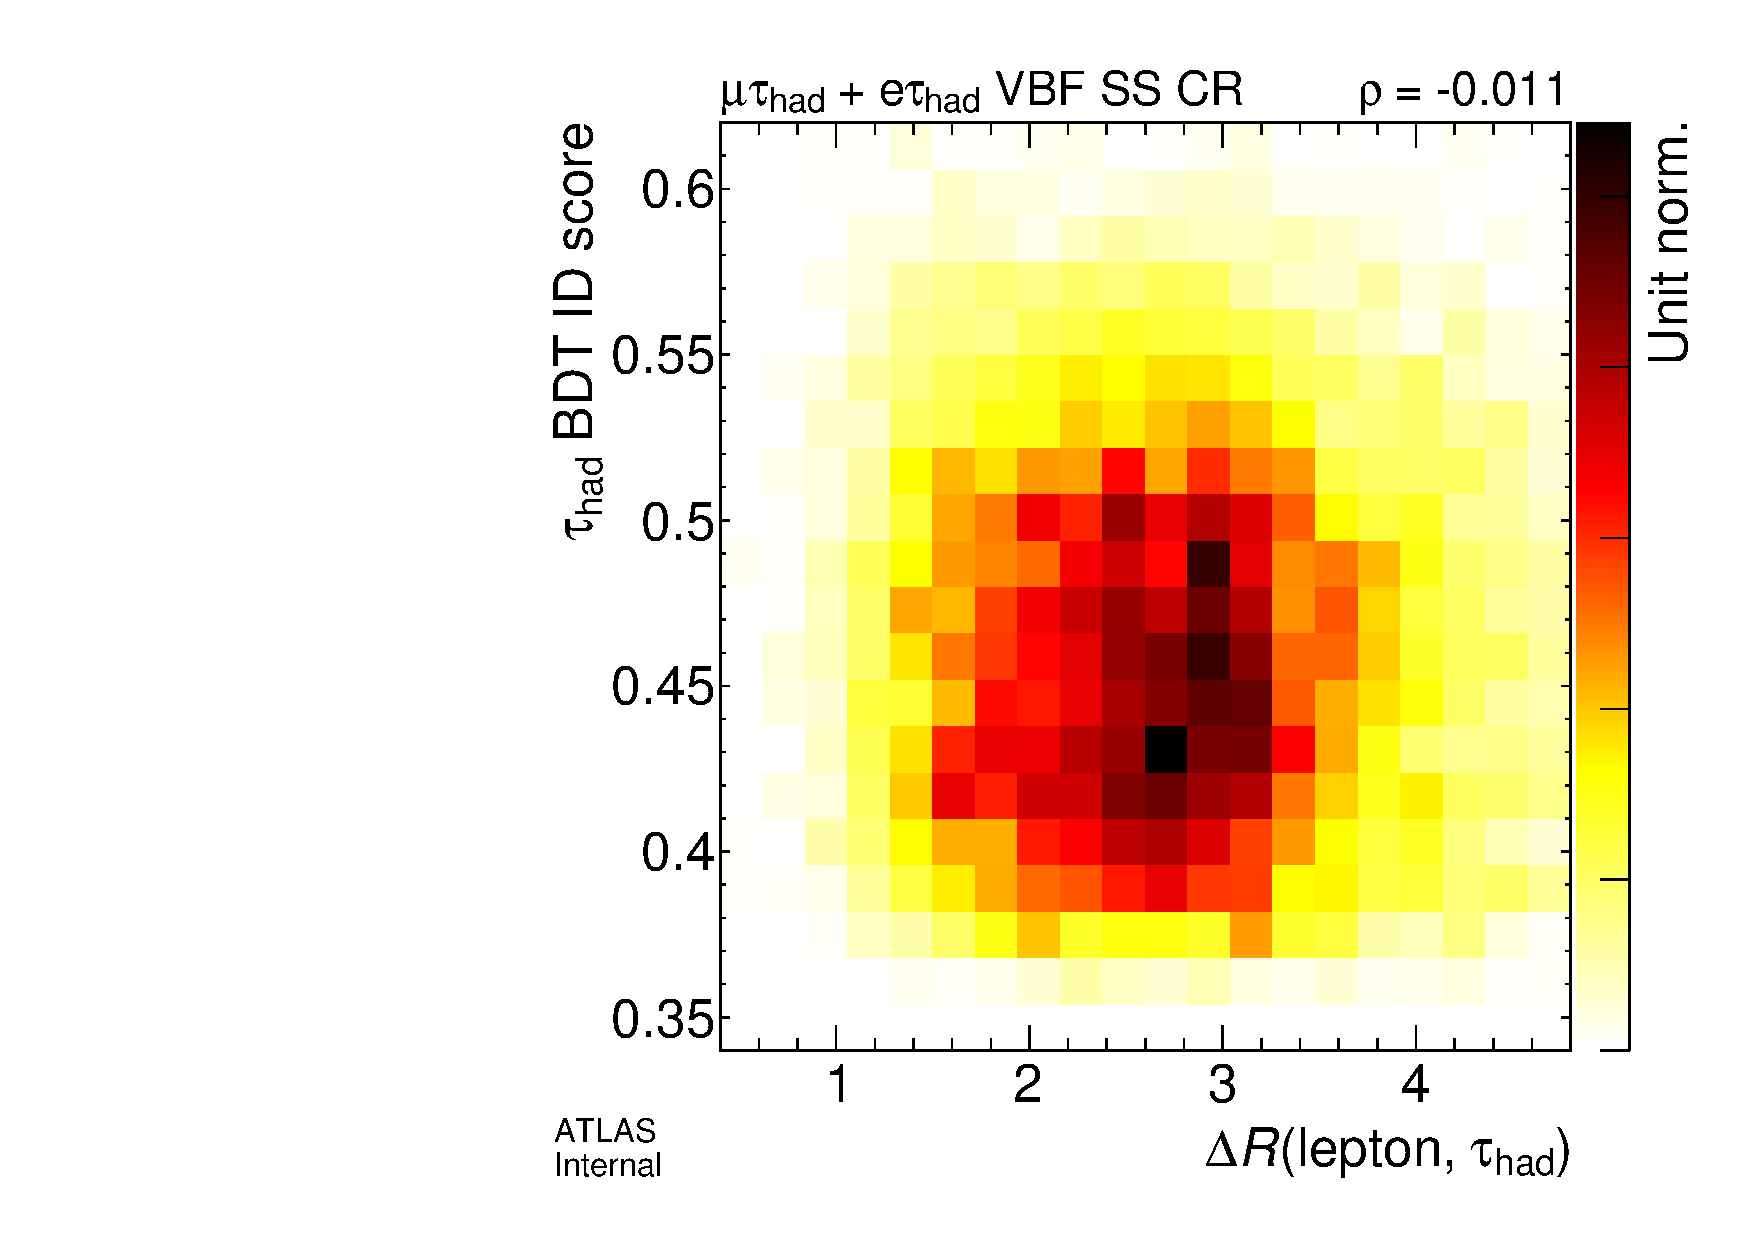
\includegraphics[width=0.32\textwidth]{figures/tauidcorrelations/tauid_vs_dR}
  % --------------
  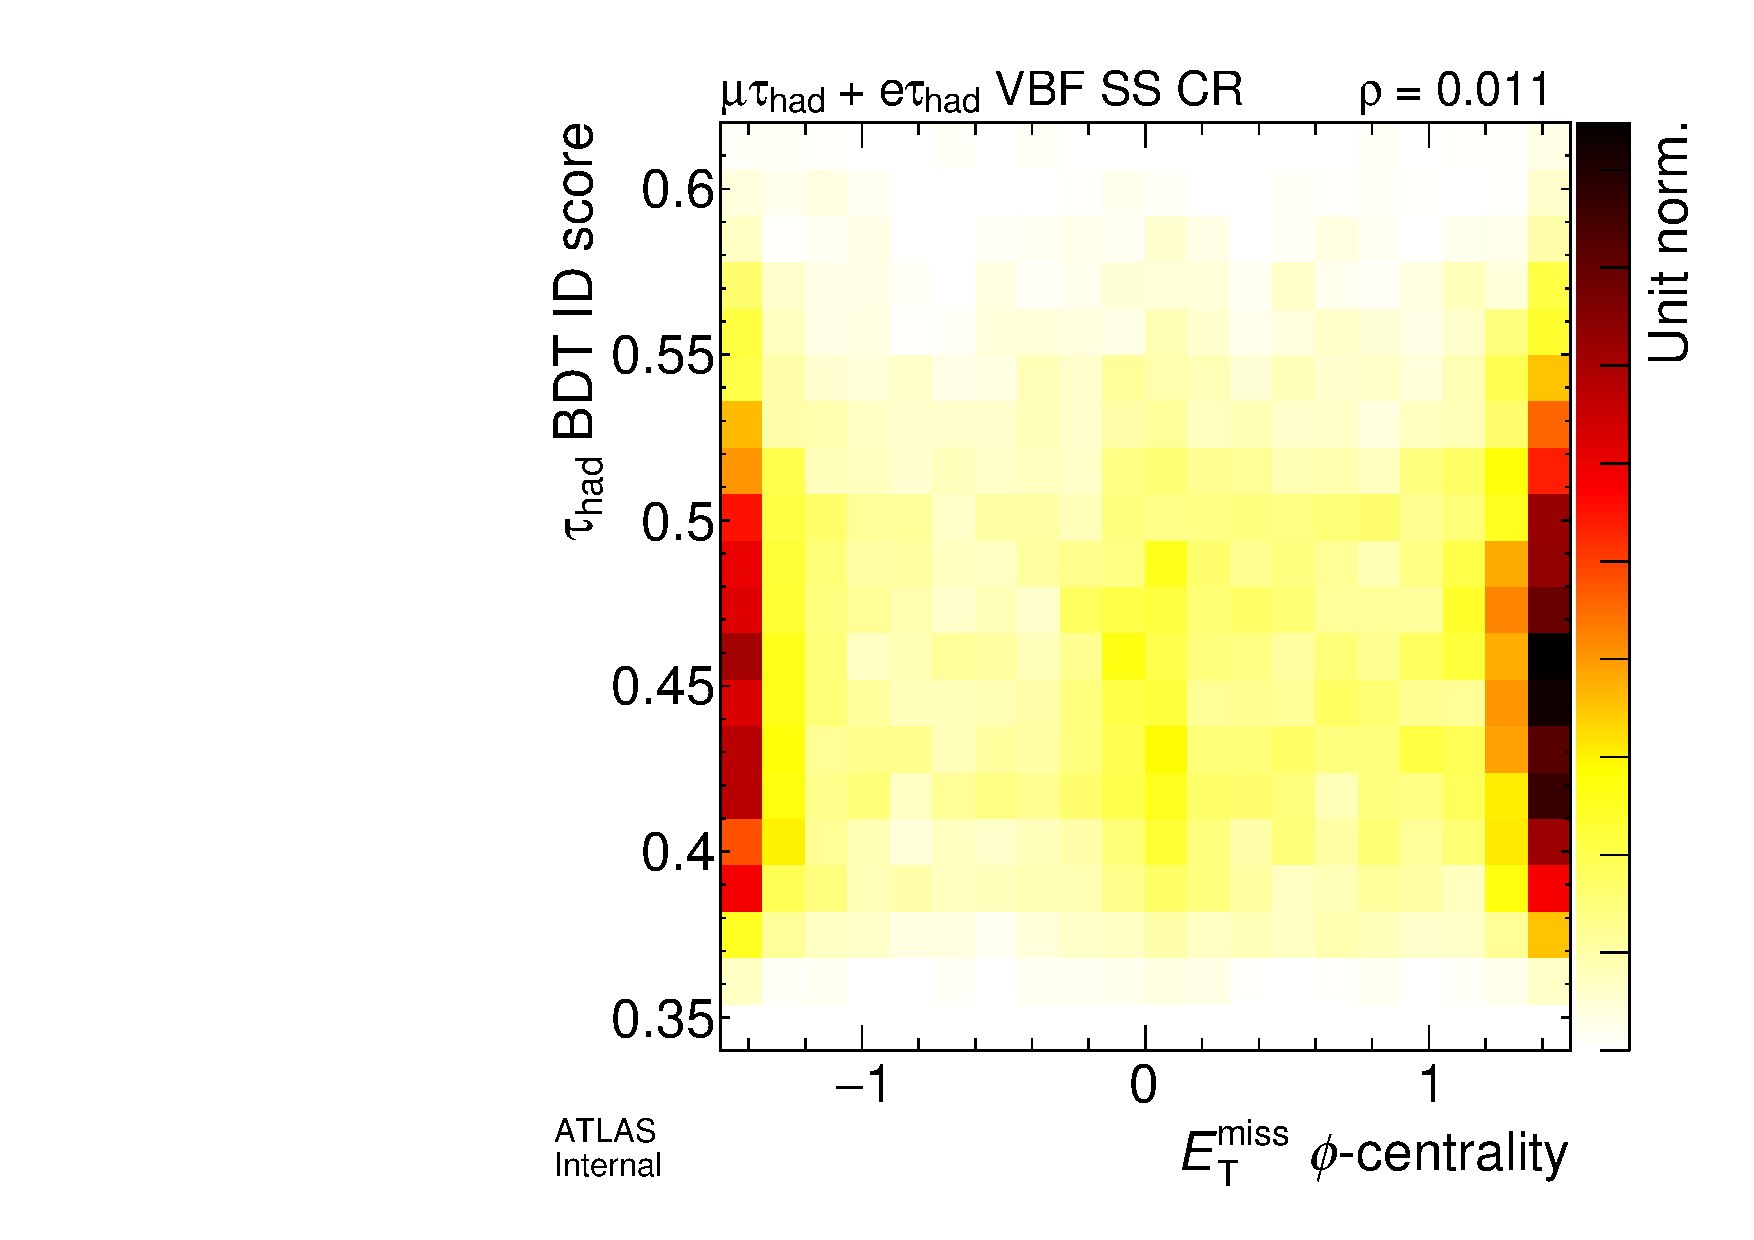
\includegraphics[width=0.32\textwidth]{figures/tauidcorrelations/tauid_vs_metphi}
  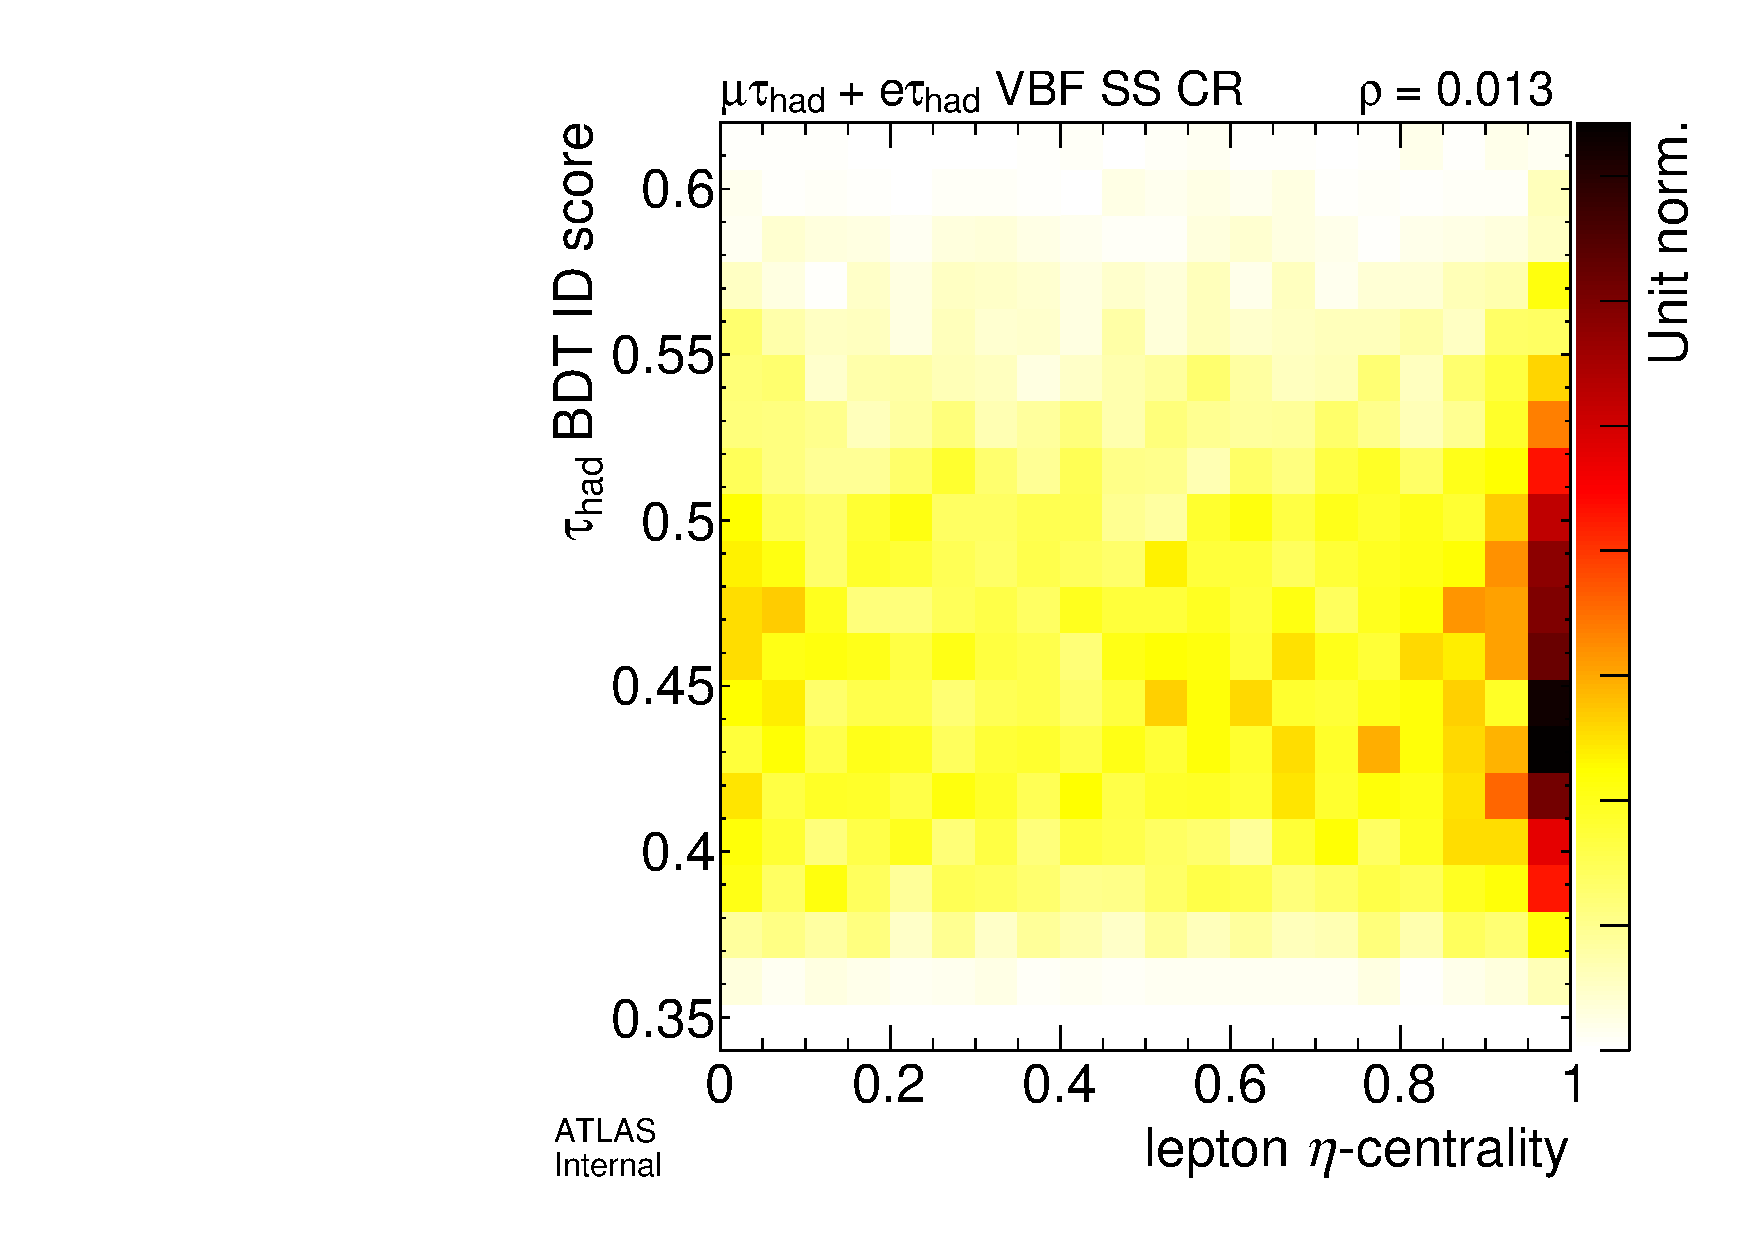
\includegraphics[width=0.32\textwidth]{figures/tauidcorrelations/tauid_vs_lepeta}
  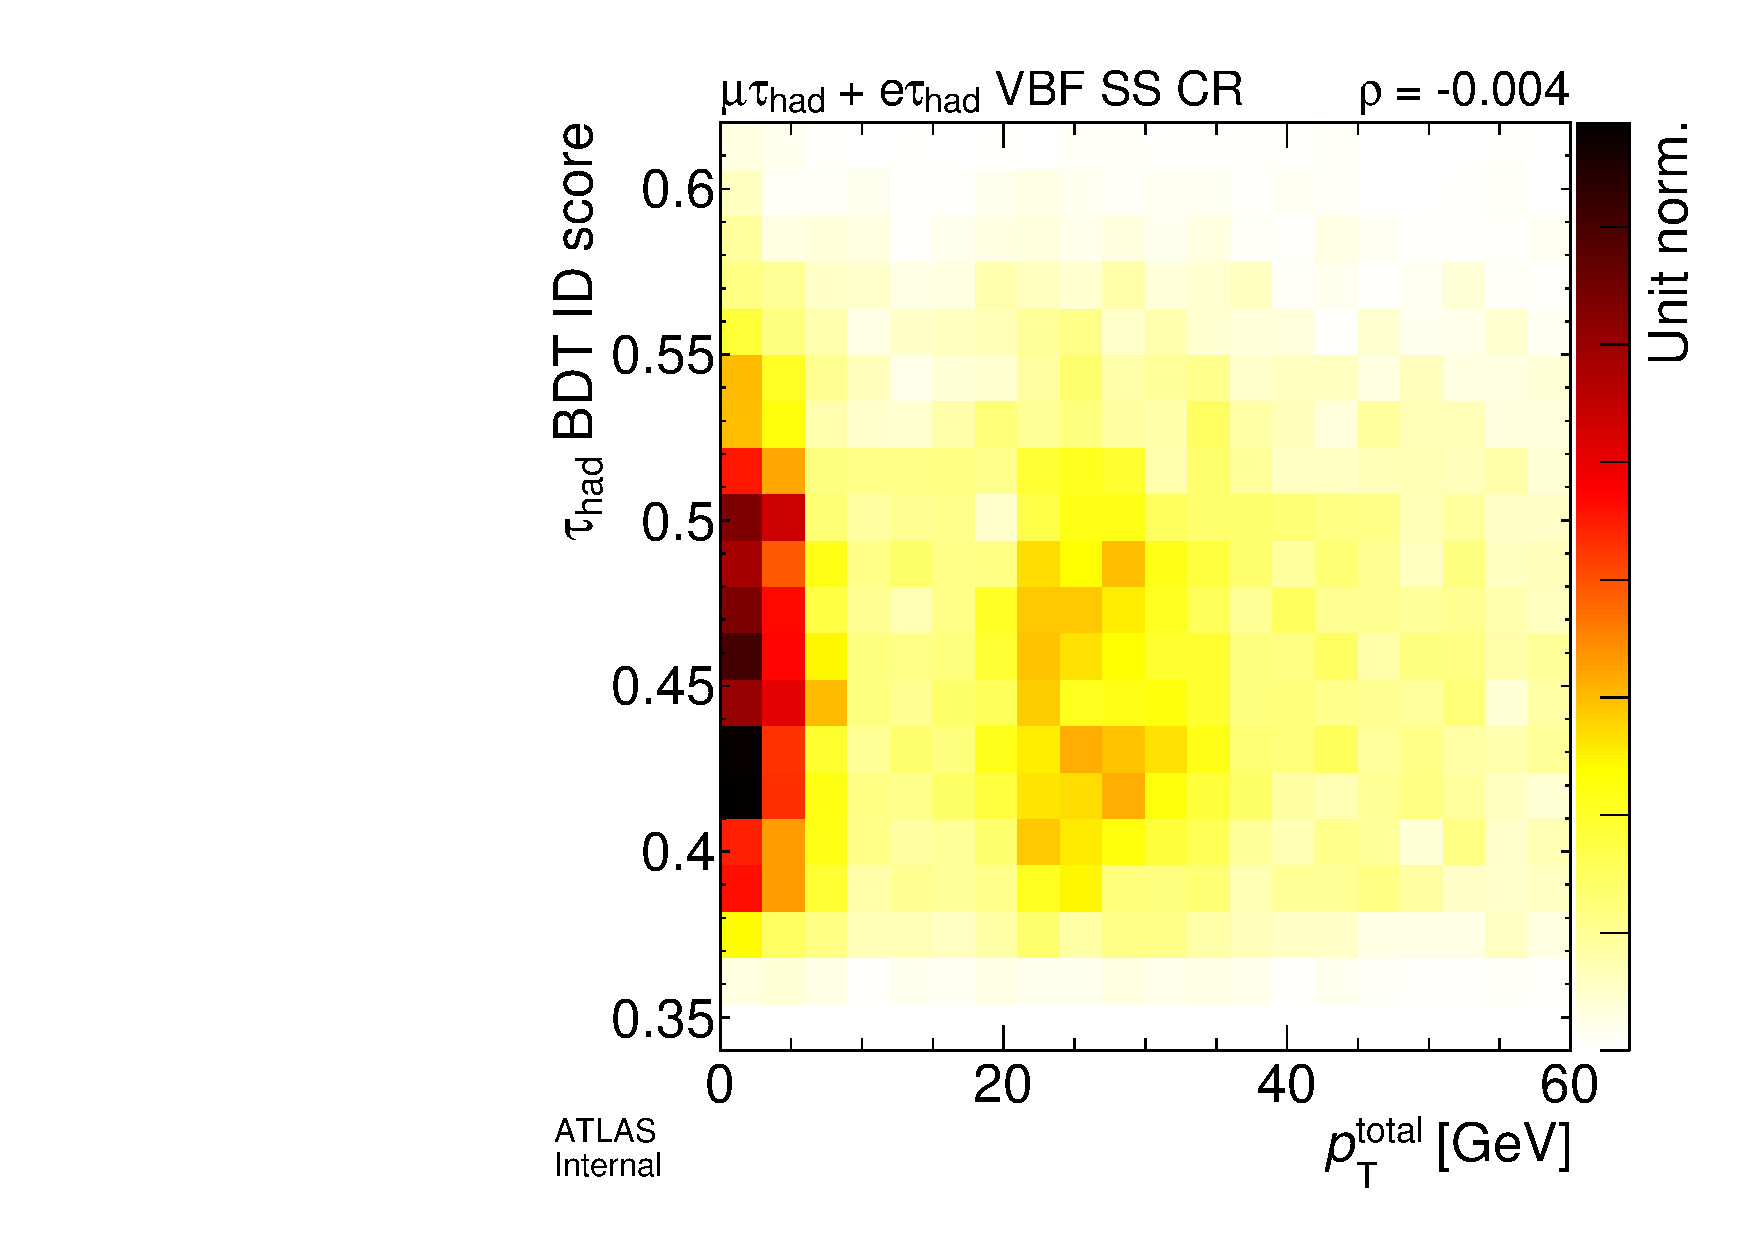
\includegraphics[width=0.32\textwidth]{figures/tauidcorrelations/tauid_vs_pttot}
  % --------------
  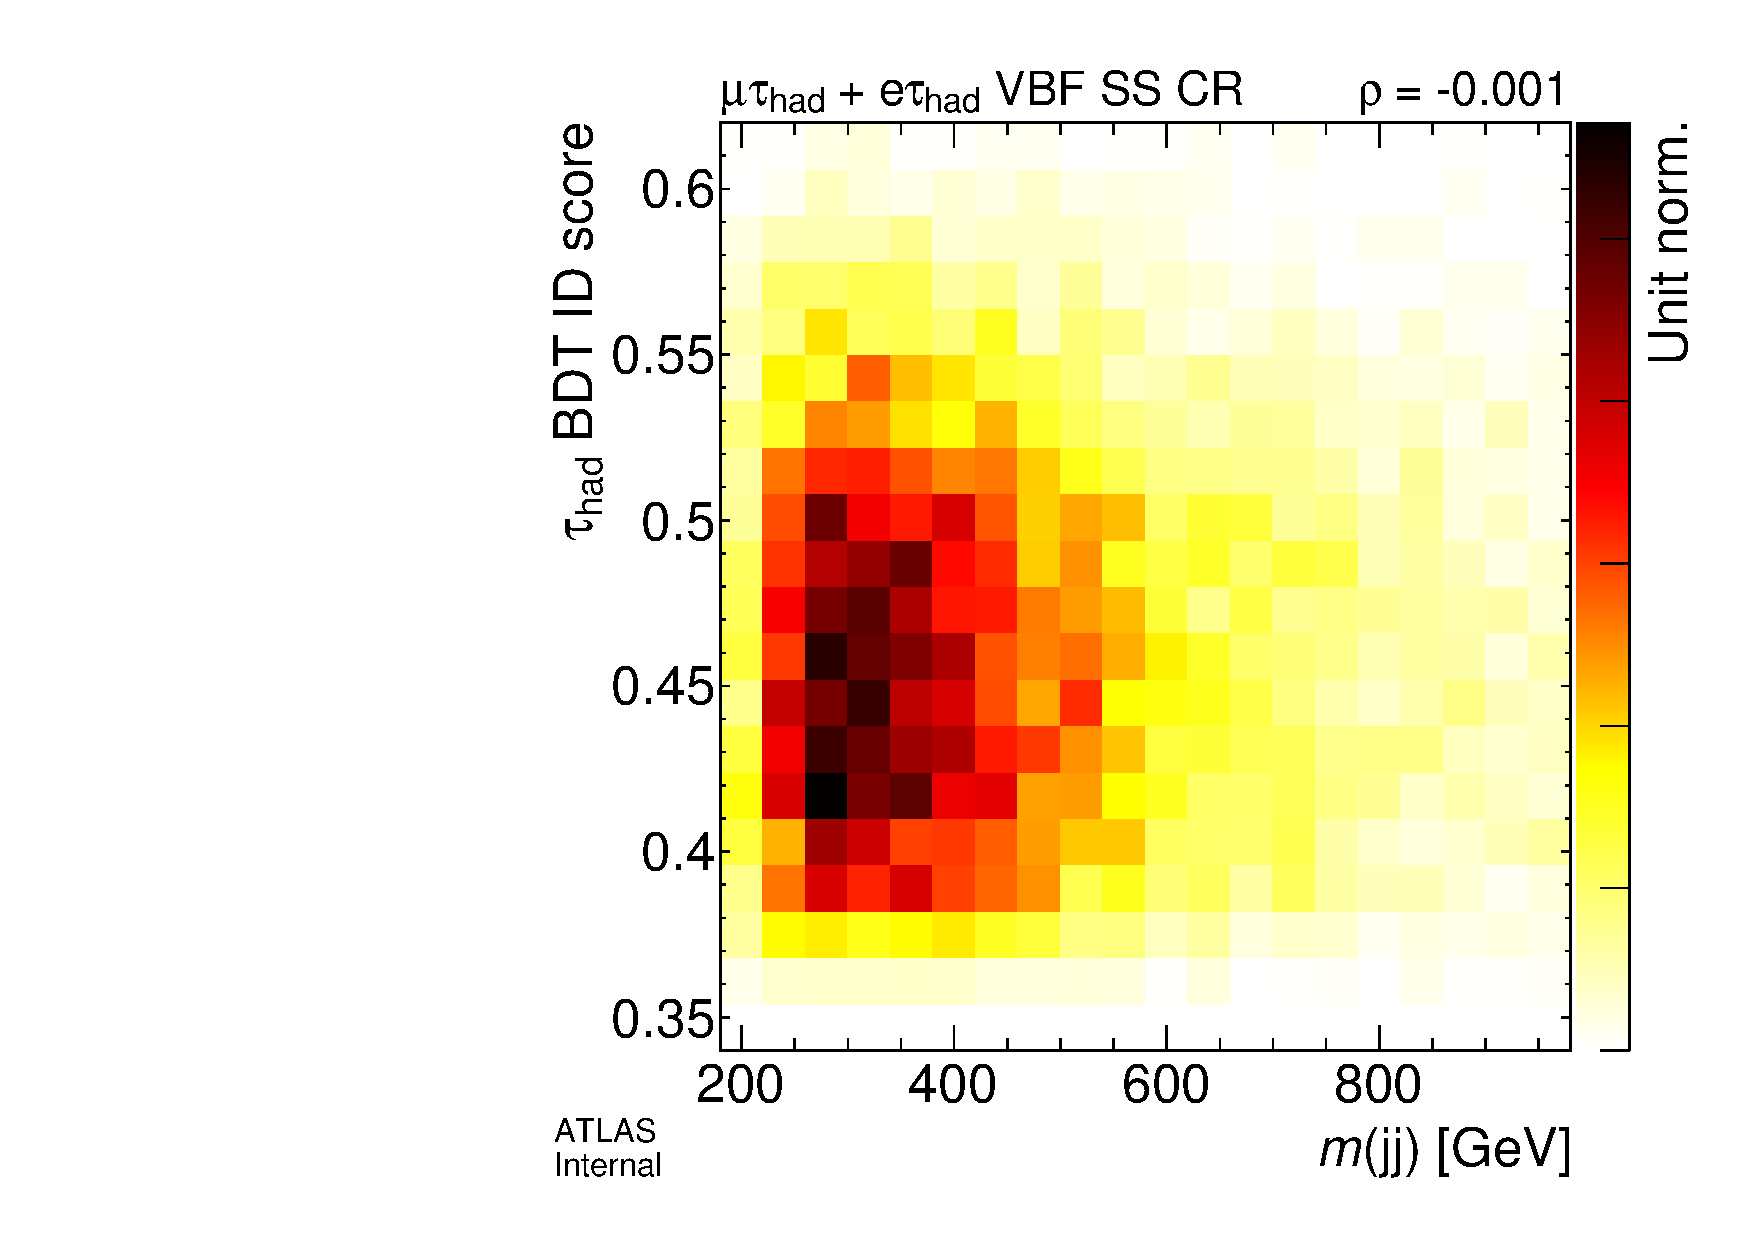
\includegraphics[width=0.32\textwidth]{figures/tauidcorrelations/tauid_vs_mjj}
  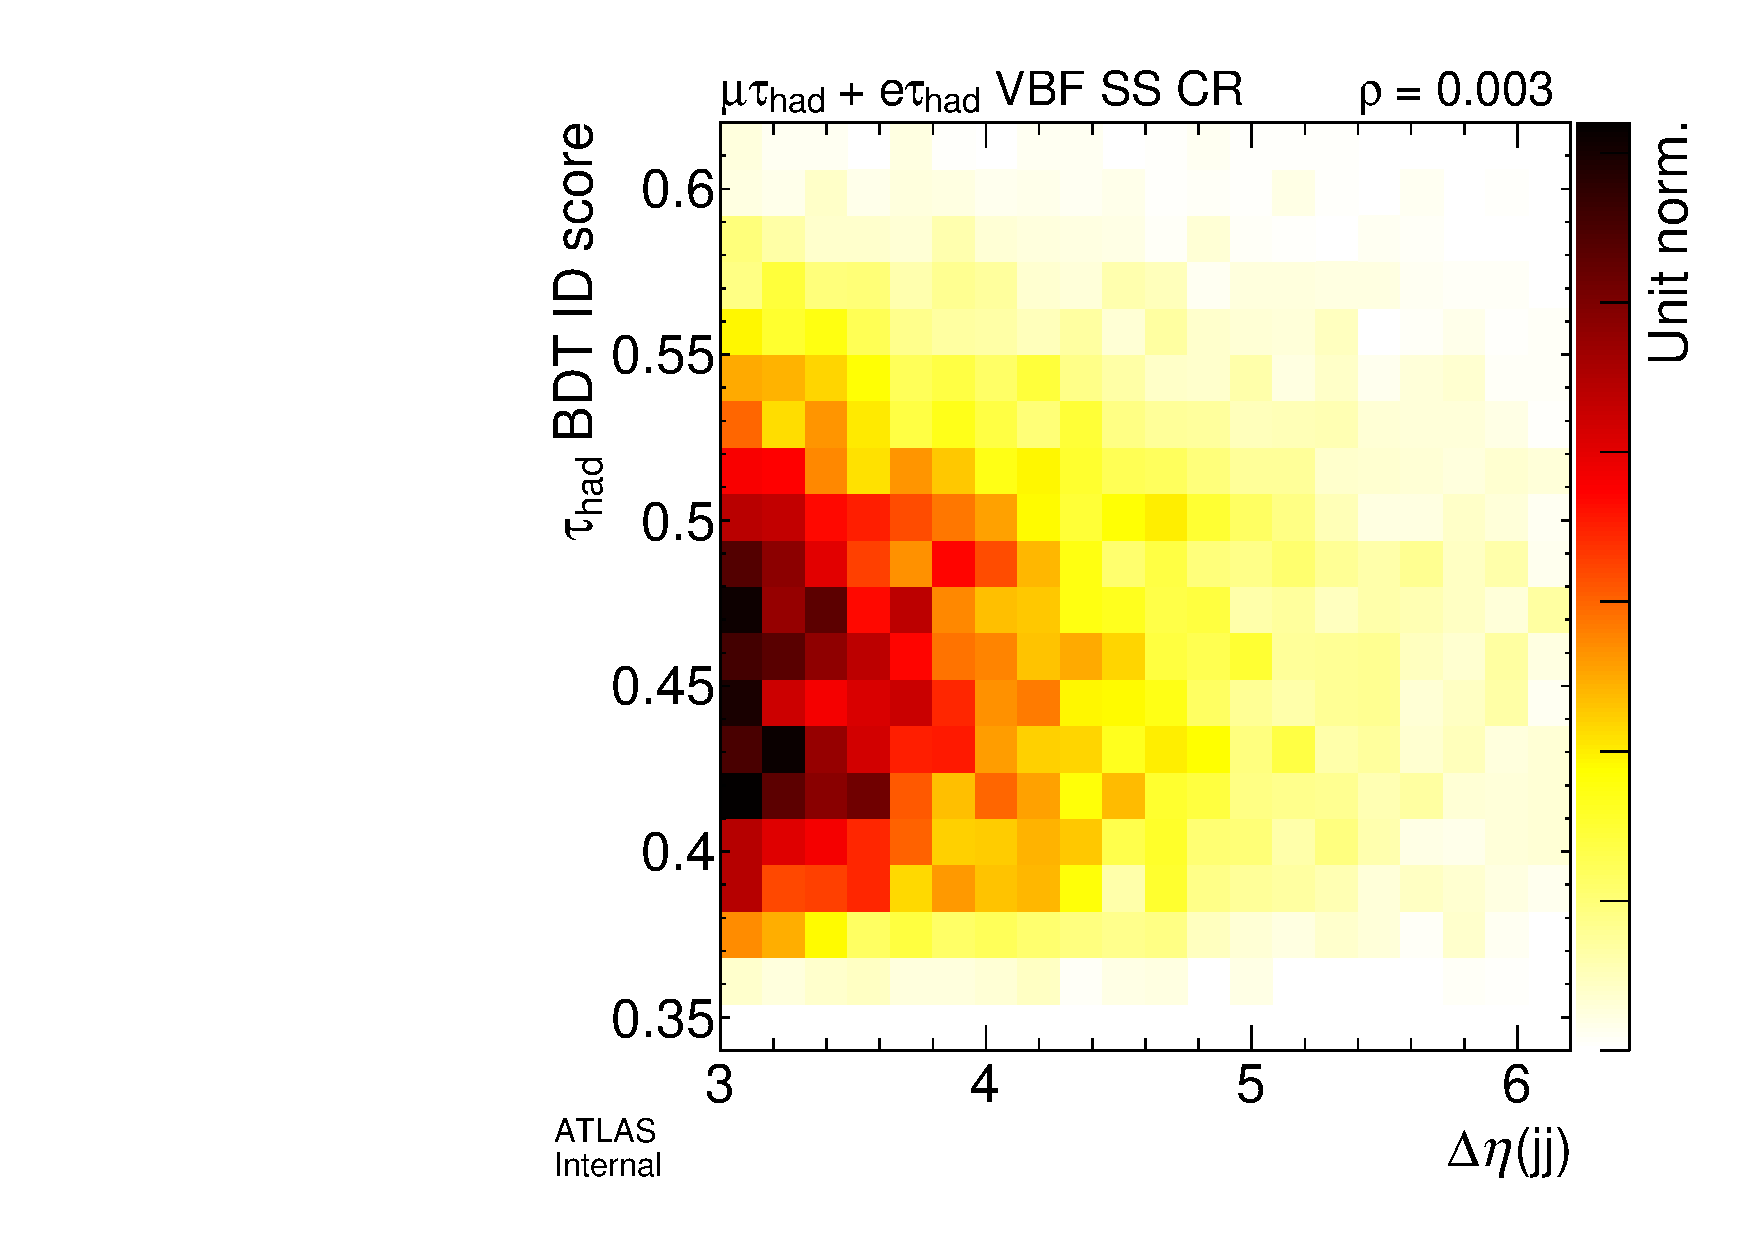
\includegraphics[width=0.32\textwidth]{figures/tauidcorrelations/tauid_vs_detajj}
  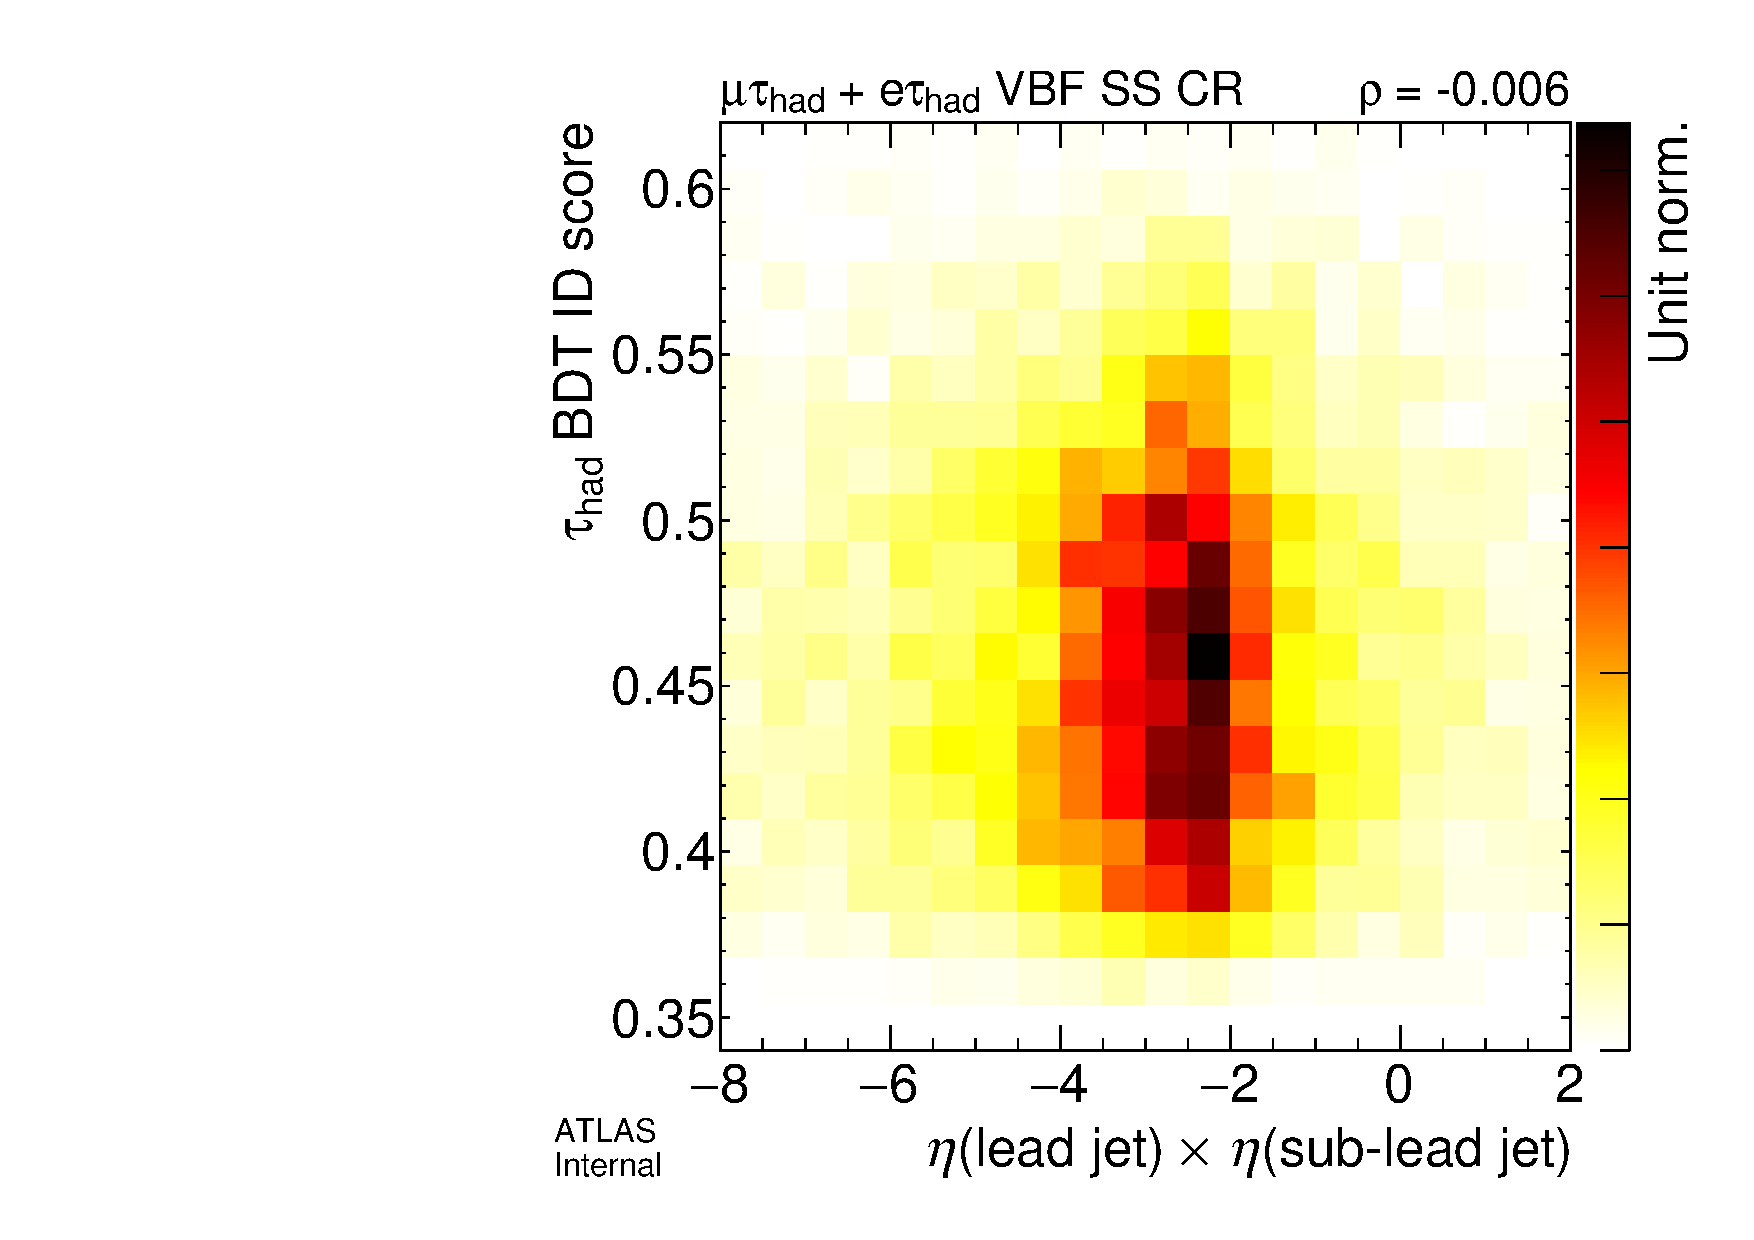
\includegraphics[width=0.32\textwidth]{figures/tauidcorrelations/tauid_vs_etaprod}
  % --------------
  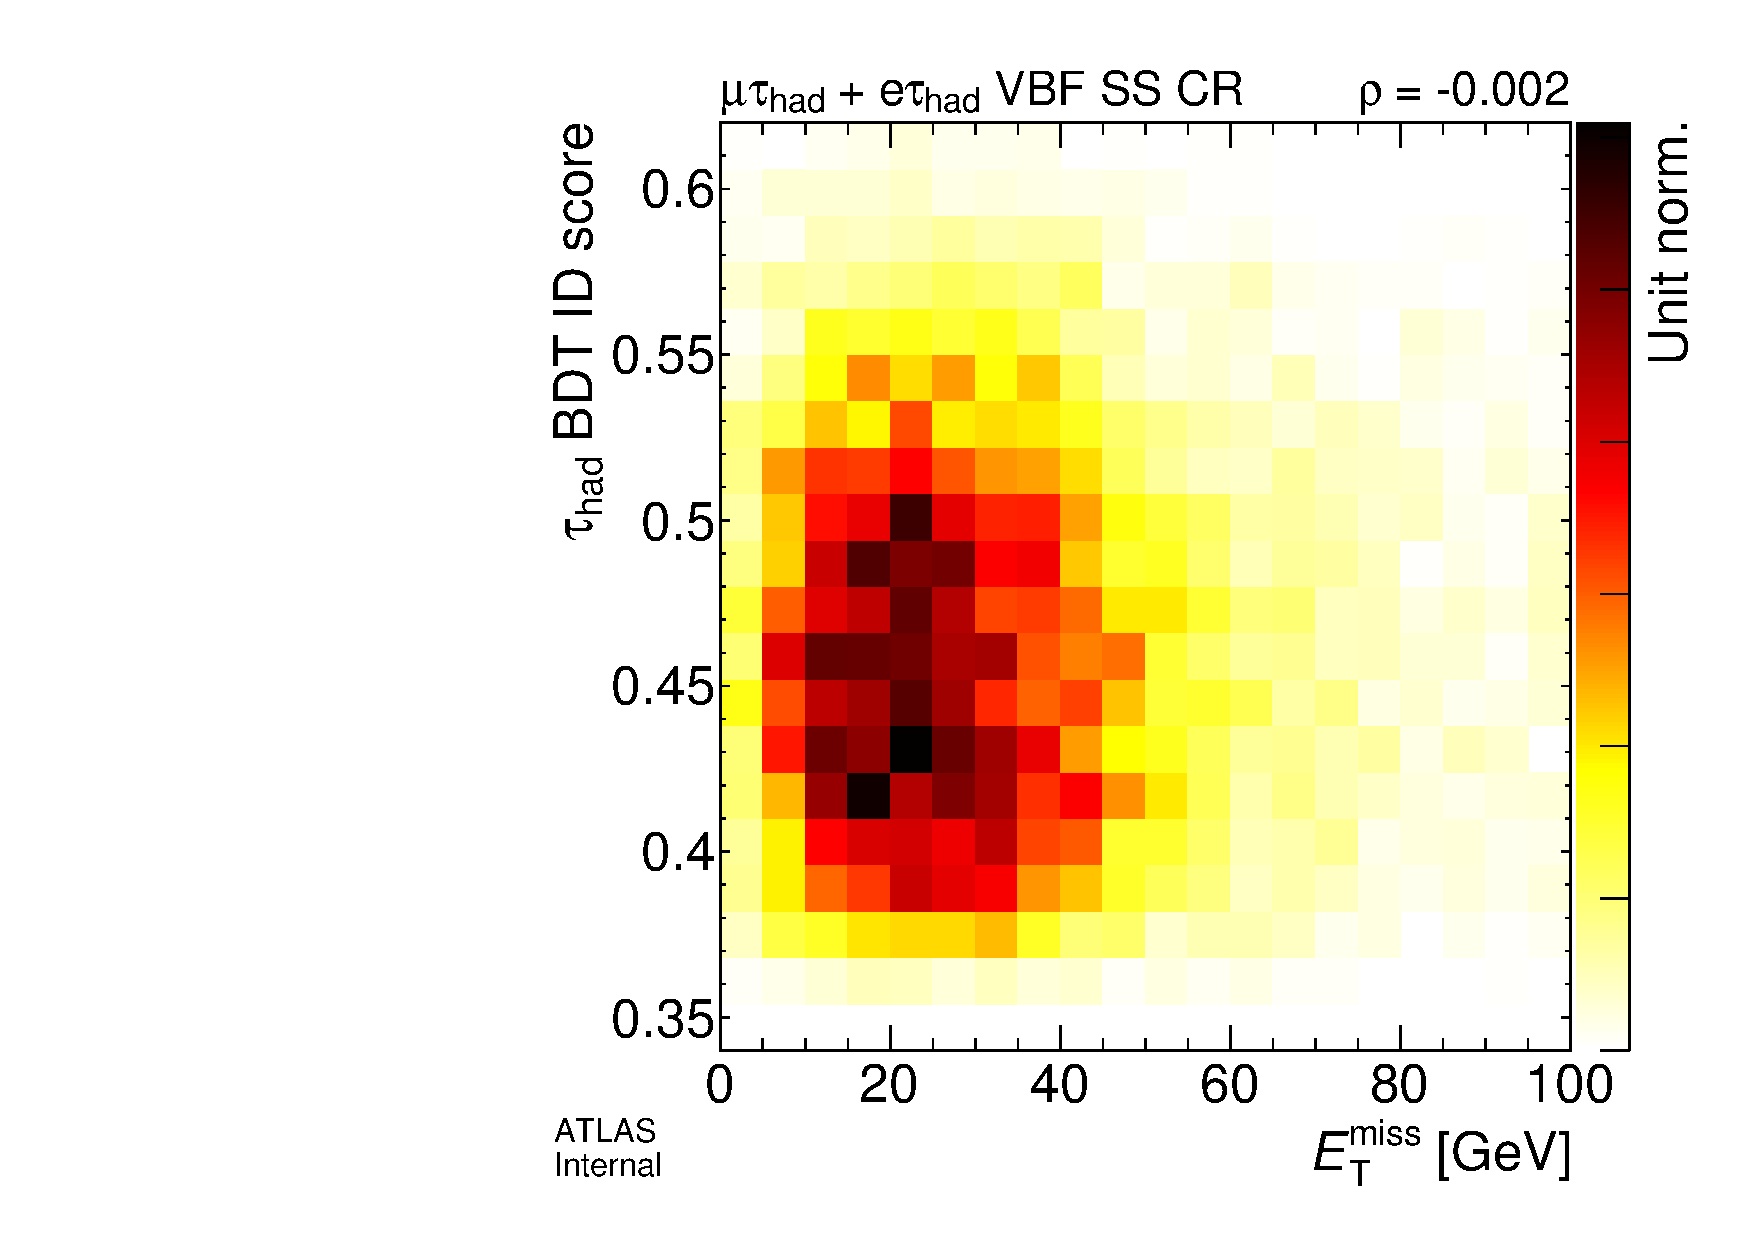
\includegraphics[width=0.32\textwidth]{figures/tauidcorrelations/tauid_vs_metet}
  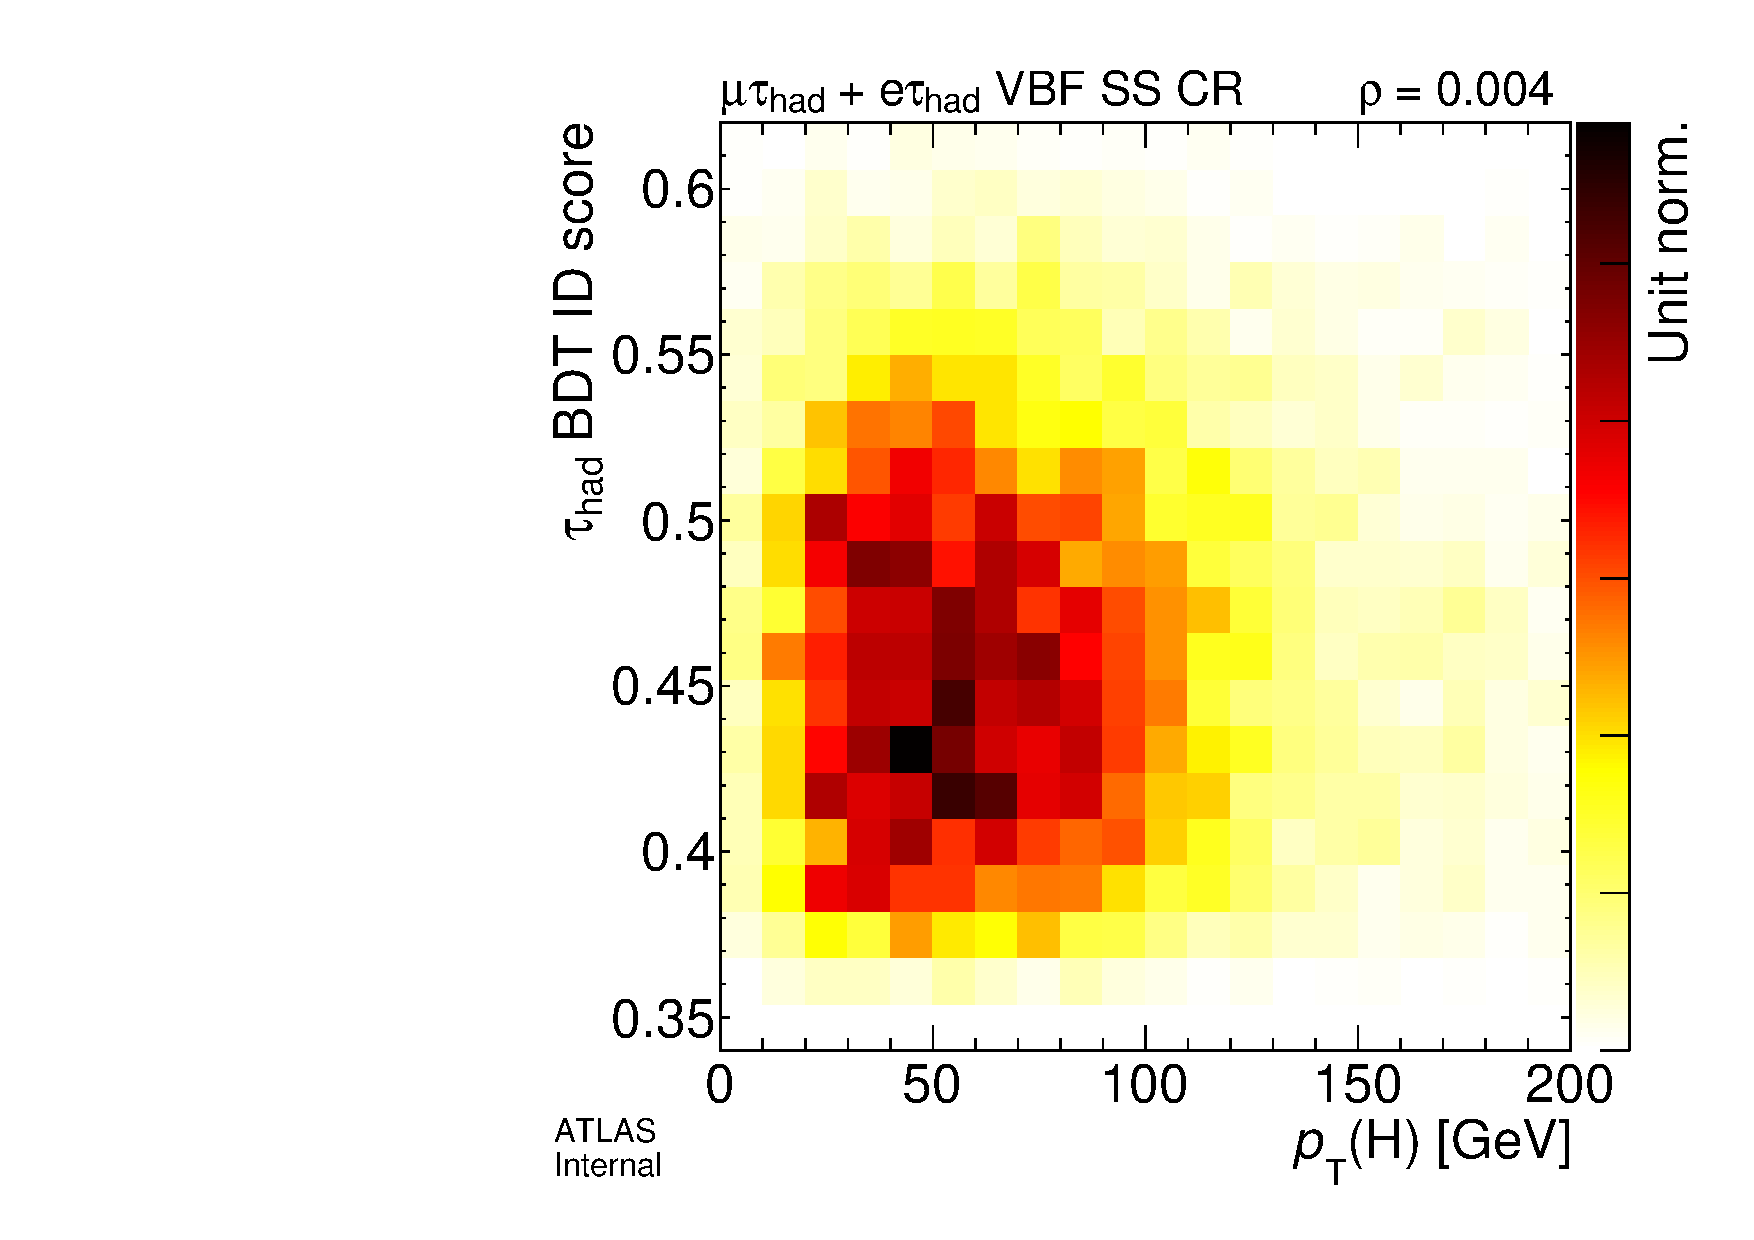
\includegraphics[width=0.32\textwidth]{figures/tauidcorrelations/tauid_vs_Hpt}
  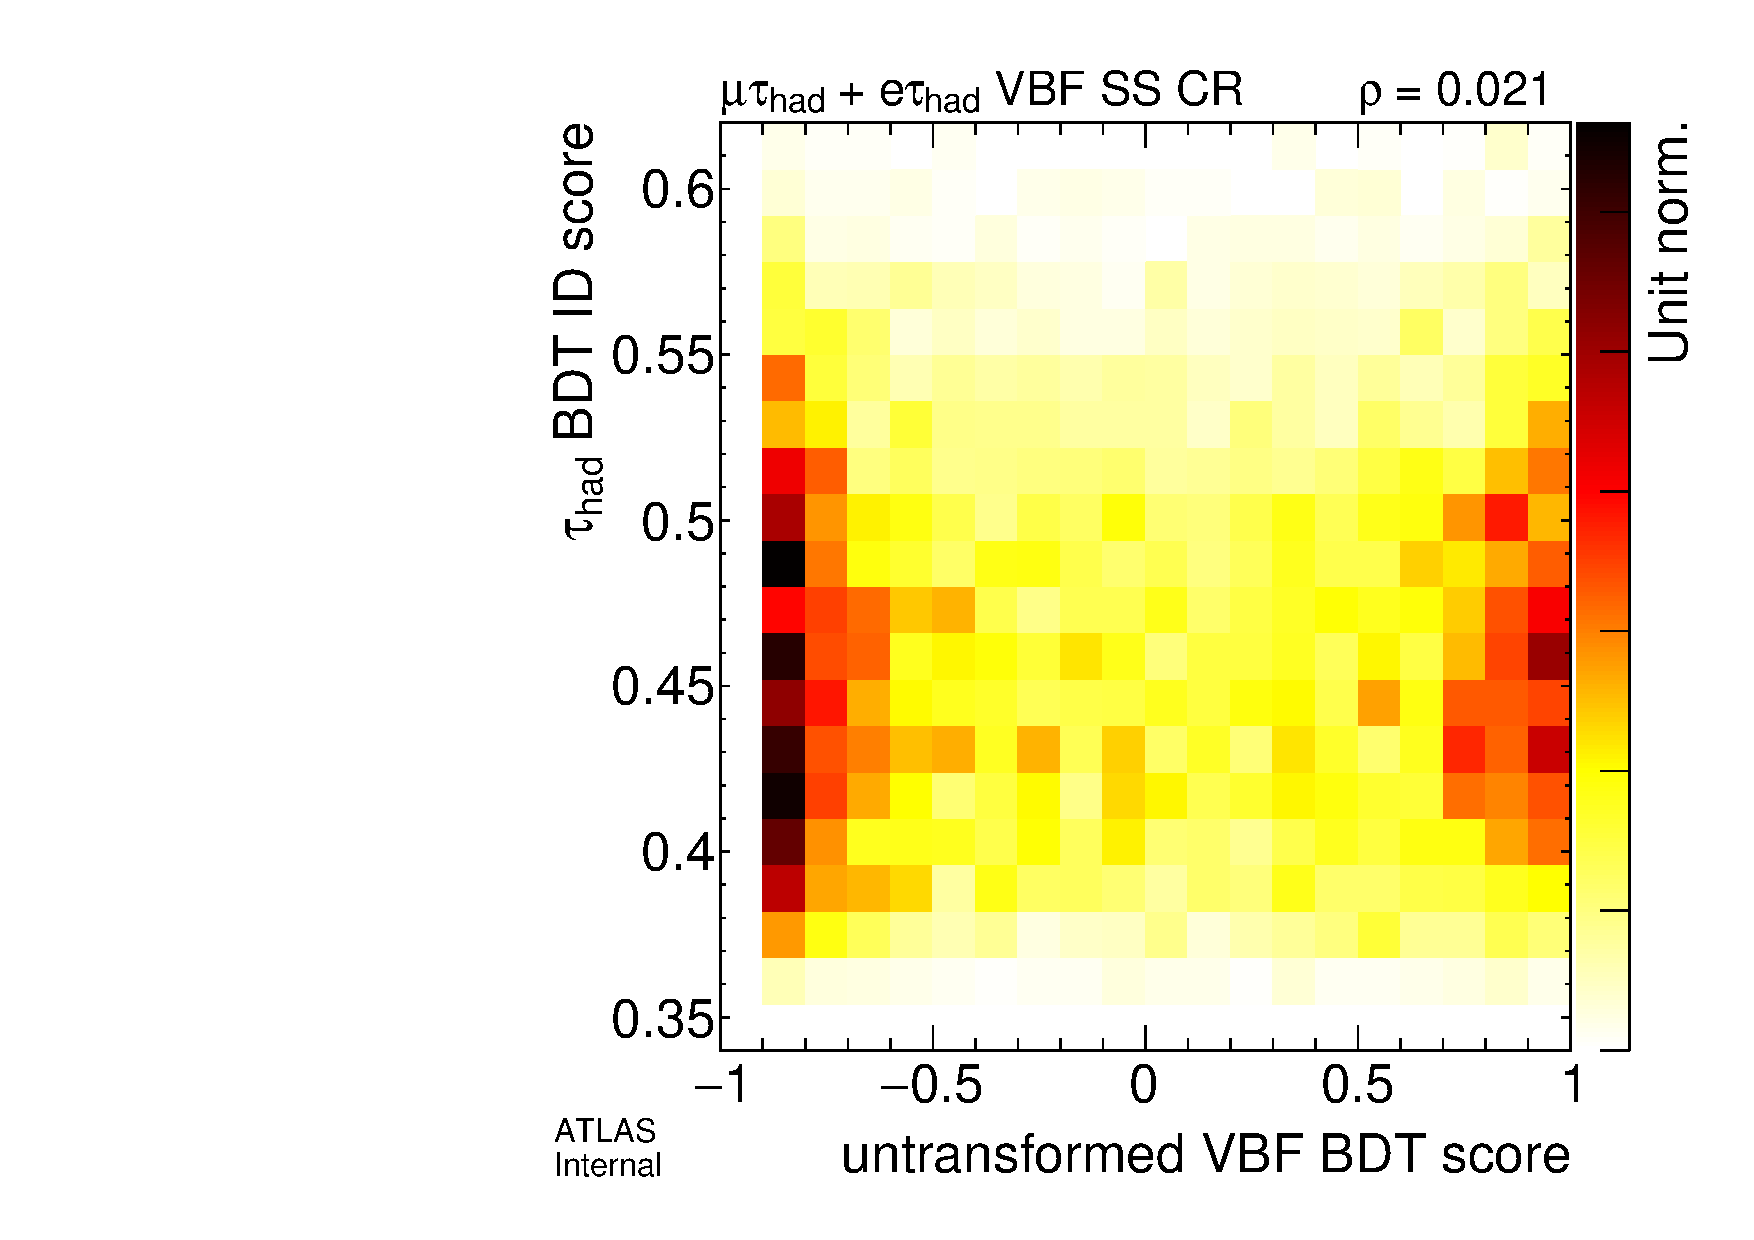
\includegraphics[width=0.32\textwidth]{figures/tauidcorrelations/tauid_vs_bdt}
  \caption{Correlations between the $\tauh$ BDT identification score and event kinematics in data events in the VBF same-sign region which fail $\tauh$ identification but fulfill all other requirements. No strong correlations are observed.}
  \label{fig:backgrounds-tauid-correlations}
\end{figure}

\clearpage

\begin{figure}[tp]
  \centering
  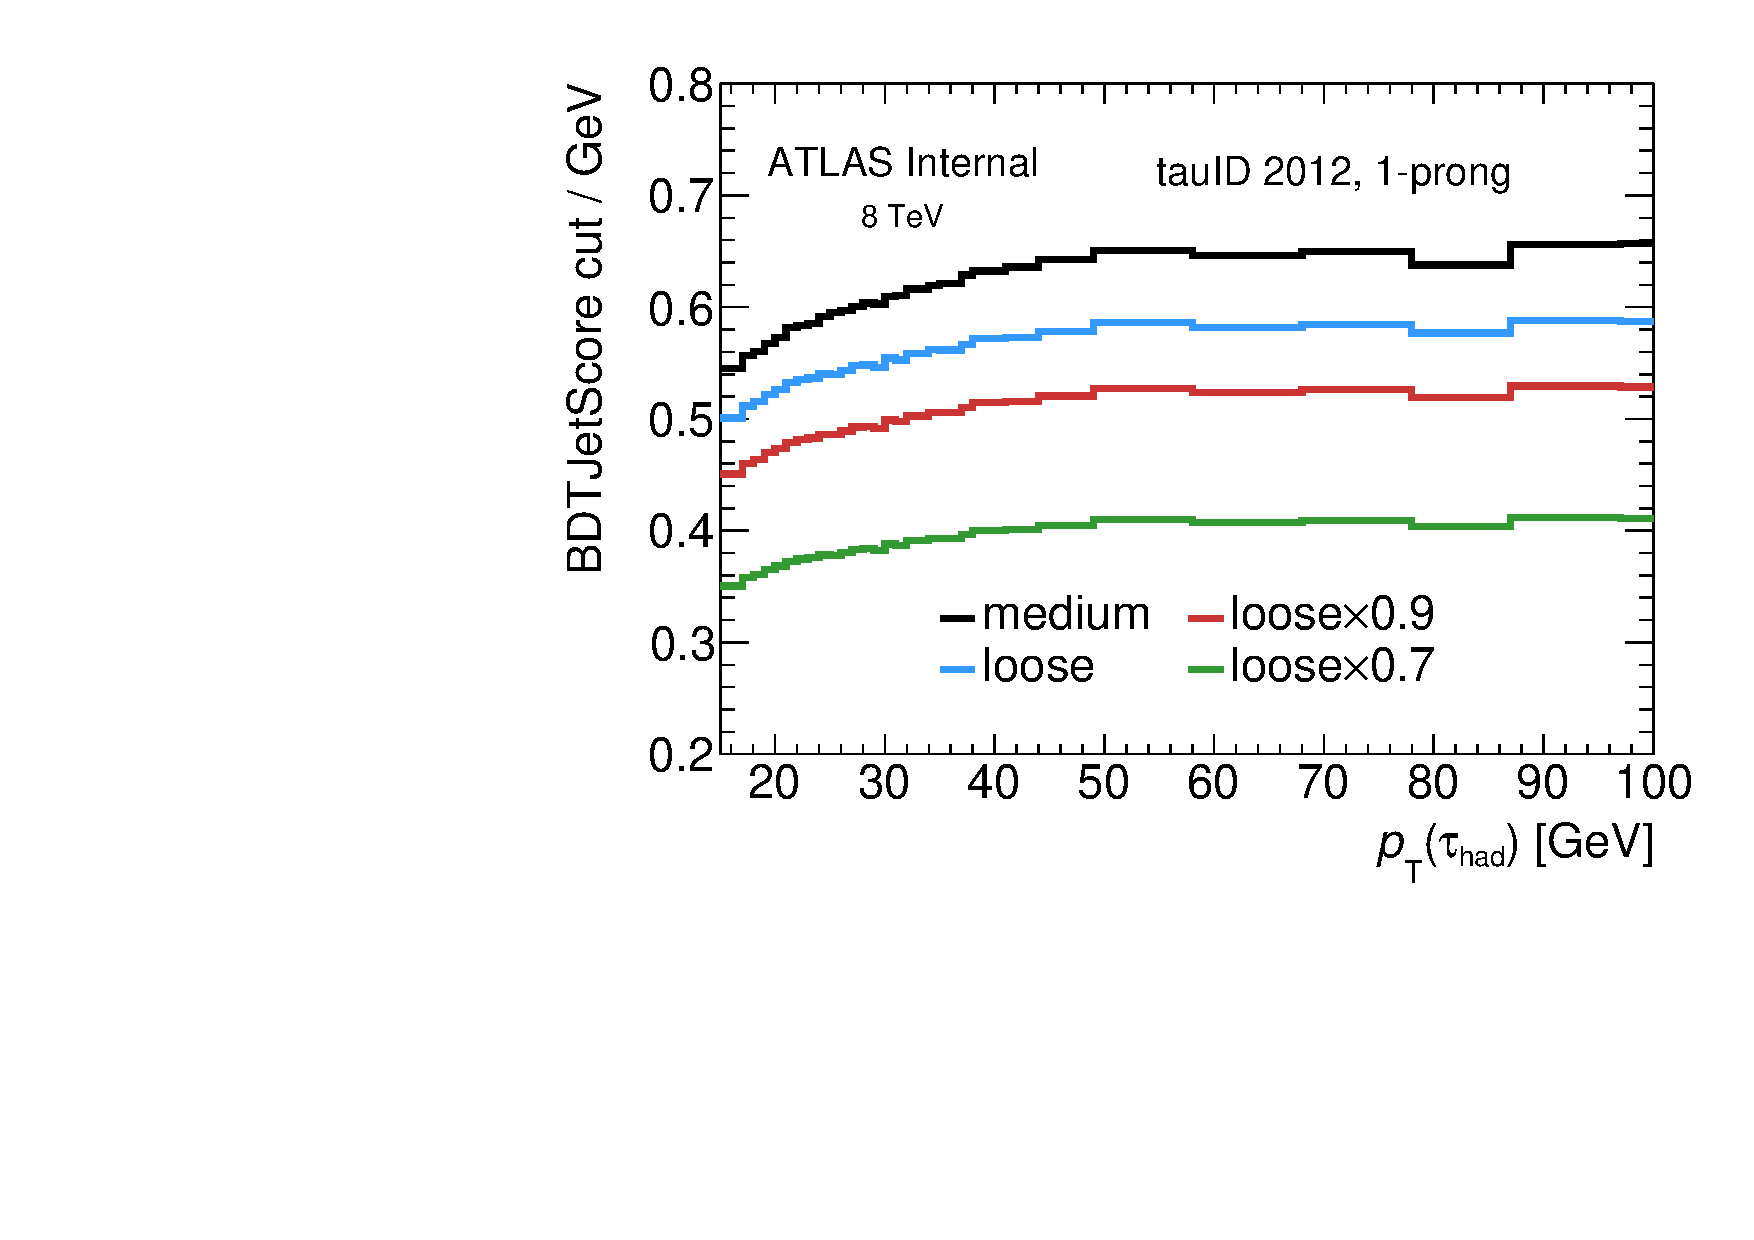
\includegraphics[width=0.48\textwidth]{figures/backgrounds/jetBDT-1p}
  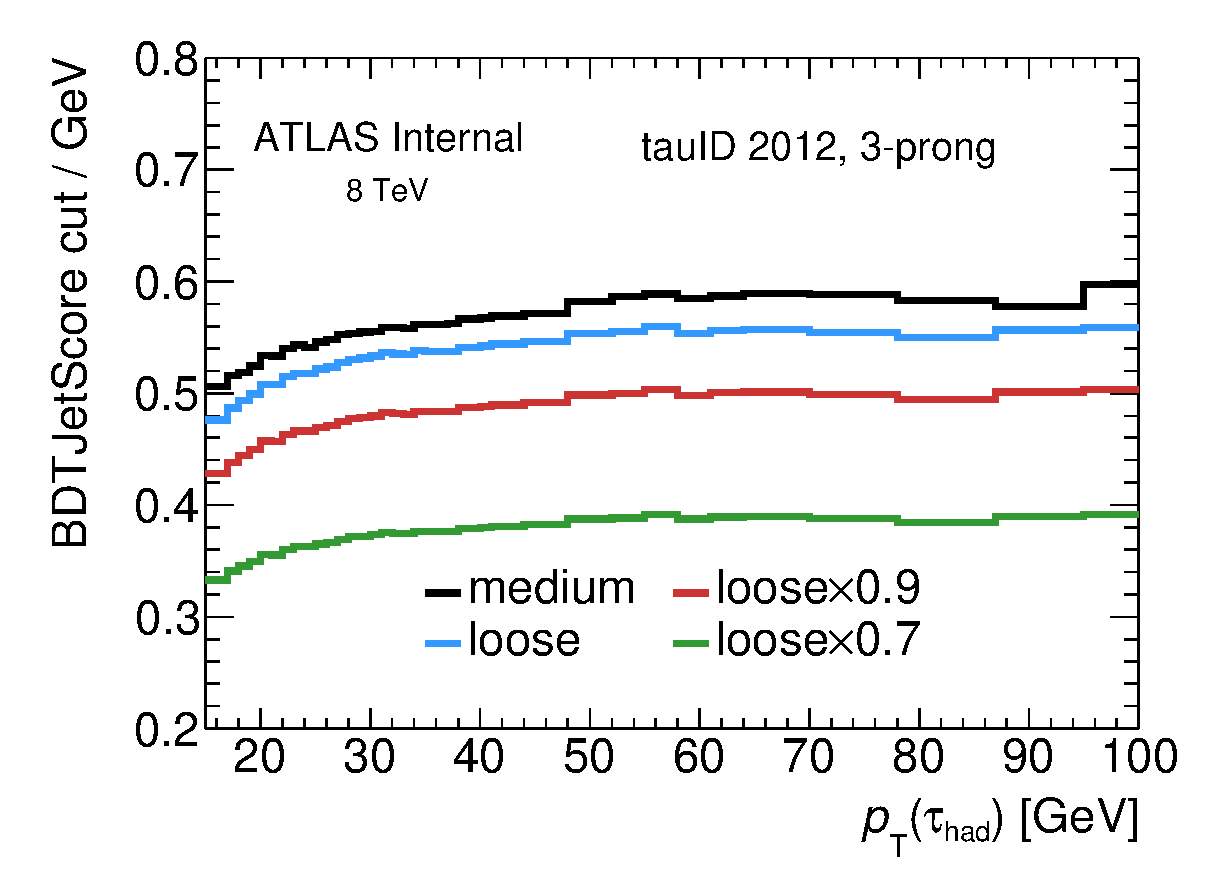
\includegraphics[width=0.48\textwidth]{figures/backgrounds/jetBDT-3p}
  \caption{Requirements on the $\tauh$ jet discriminant, which are defined to have constant signal efficiency as a function of $\pt(\tauh)$, of various operating points for 1-track $\tauh$ (left) and 3-track $\tauh$ (right).}
  \label{fig:backgrounds-workingpoints}
\end{figure}

\begin{figure}[tp]
  \centering
  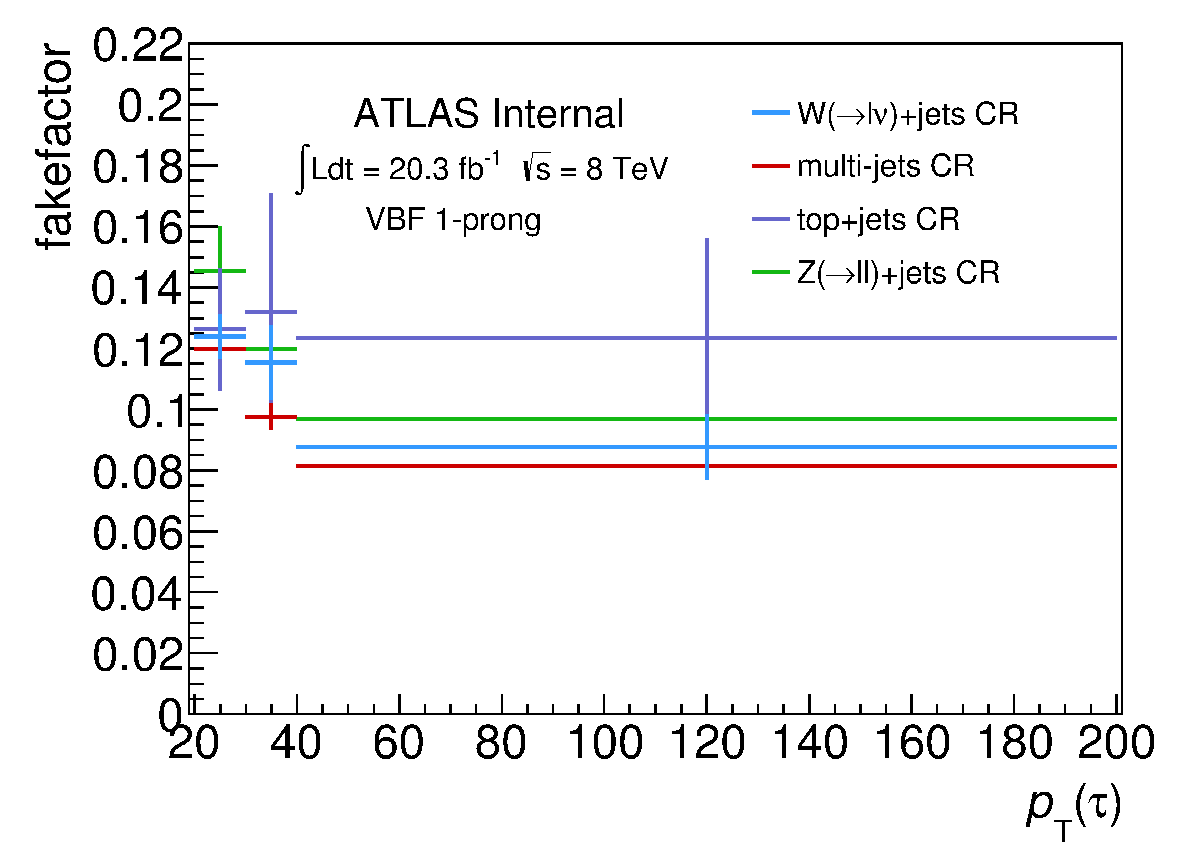
\includegraphics[width=0.48\textwidth]{figures/backgrounds/fakefactor_8TeV_vbf_1p_CRs}
  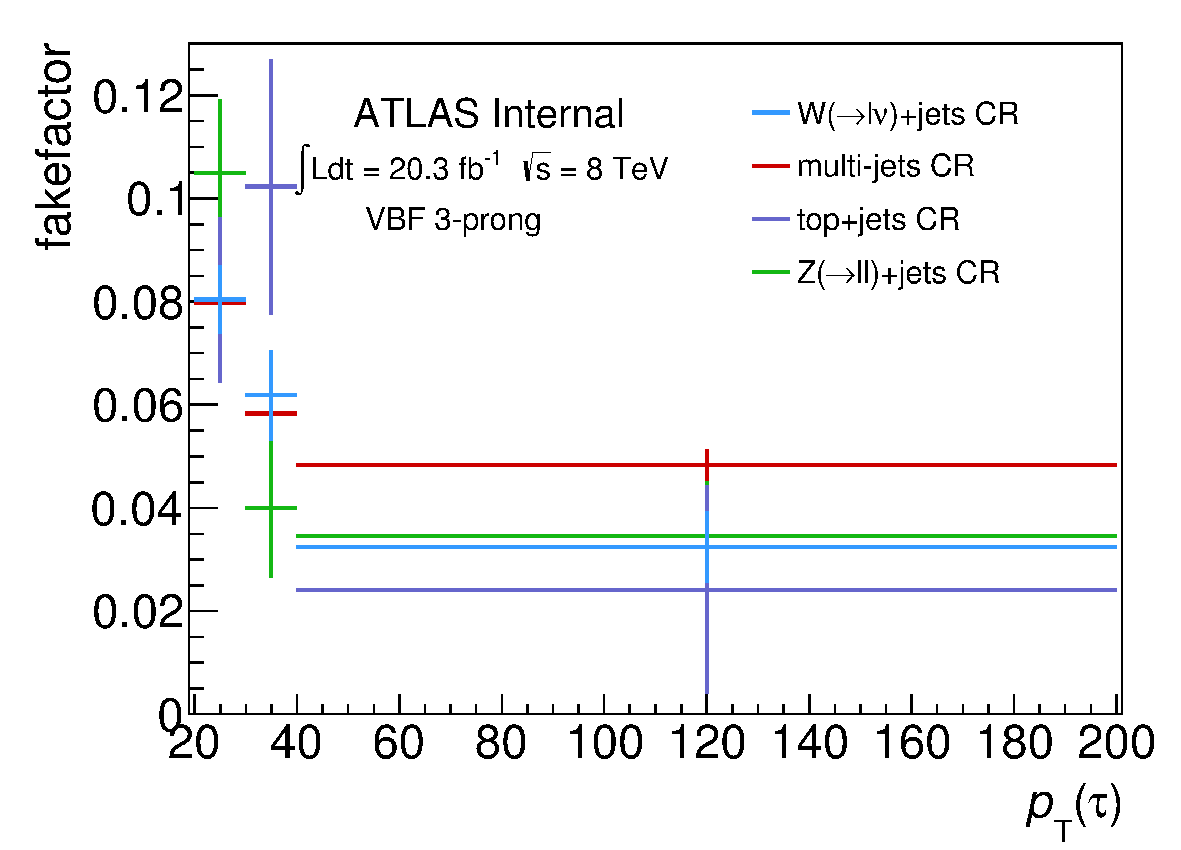
\includegraphics[width=0.48\textwidth]{figures/backgrounds/fakefactor_8TeV_vbf_3p_CRs}
  \caption{Fake factors in the VBF category measured in the various control regions in data for 1-track $\tauh$ (left) and 3-track $\tauh$ (right).}
  \label{fig:backgrounds-fakefactorsVBFCRs}
\end{figure}

\subsection{Composition of $\fakes$ in the SR}

\begin{figure}[tp]
  \centering
  \includegraphics[width=0.90\textwidth]{figures/backgrounds/rx-vbf}
  \caption{A pie chart of the composition of $\fakes$ processes in the anti-identified CR as predicted by simulation and data (left) and the systematic variations on the composition (right).}
  \label{fig:backgrounds-rx-vbf}
\end{figure}

\clearpage

\begin{figure}[tp]
  \centering
  \includegraphics[width=0.32\textwidth]{figures/rx/vbf-mvaSR/tau-pt}
  \includegraphics[width=0.32\textwidth]{figures/rx/vbf-mvaSR/tau-eta}
  \includegraphics[width=0.32\textwidth]{figures/rx/vbf-mvaSR/tau-numTrack}
  % --------------
  \includegraphics[width=0.32\textwidth]{figures/rx/vbf-mvaSR/lep-pt-hi}
  \includegraphics[width=0.32\textwidth]{figures/rx/vbf-mvaSR/lep-eta}
  \includegraphics[width=0.32\textwidth]{figures/rx/vbf-mvaSR/taulep-dR}
  % --------------
  \includegraphics[width=0.32\textwidth]{figures/rx/vbf-mvaSR/met-pt-hi}
  \includegraphics[width=0.32\textwidth]{figures/rx/vbf-mvaSR/mMMC}
  \includegraphics[width=0.32\textwidth]{figures/rx/vbf-mvaSR/mT}
  % --------------
  \includegraphics[width=0.32\textwidth]{figures/rx/vbf-mvaSR/met-phi-centrality}
  \includegraphics[width=0.32\textwidth]{figures/rx/vbf-mvaSR/H-pt-hi}
  \includegraphics[width=0.32\textwidth]{figures/rx/vbf-mvaSR/mvis}
  \caption{The composition of $\fakes$ processes in the anti-identified CR as predicted by simulation and data as a function of event kinematics.}
  \label{fig:backgrounds-rx-vbf-taus}
\end{figure}

\clearpage

\begin{figure}[tp]
  \includegraphics[width=0.32\textwidth]{figures/rx/vbf-mvaSR/jet-1-pt}
  \includegraphics[width=0.32\textwidth]{figures/rx/vbf-mvaSR/jet-1-eta}
  \includegraphics[width=0.32\textwidth]{figures/rx/vbf-mvaSR/jets-dphi}
  % --------------
  \includegraphics[width=0.32\textwidth]{figures/rx/vbf-mvaSR/jet-2-pt}
  \includegraphics[width=0.32\textwidth]{figures/rx/vbf-mvaSR/jet-2-eta}
  \includegraphics[width=0.32\textwidth]{figures/rx/vbf-mvaSR/jets-deta}
  % --------------
  \includegraphics[width=0.32\textwidth]{figures/rx/vbf-mvaSR/jets-etaprod}
  \includegraphics[width=0.32\textwidth]{figures/rx/vbf-mvaSR/lep-eta-centrality}
  \includegraphics[width=0.32\textwidth]{figures/rx/vbf-mvaSR/system-pt}
  % --------------
  \includegraphics[width=0.32\textwidth]{figures/rx/vbf-mvaSR/n-jets30}
  \includegraphics[width=0.32\textwidth]{figures/rx/vbf-mvaSR/dijet-m-veryhigh}
  \includegraphics[width=0.32\textwidth]{figures/rx/vbf-mvaSR/BDTEve-VBF}
  \caption{The composition of $\fakes$ processes in the anti-identified CR as predicted by simulation and data as a function of event kinematics.}
  \label{fig:backgrounds-rx-vbf-jets}
\end{figure}

\begin{figure}[tp]
  \centering
  \includegraphics[width=0.48\textwidth]{figures/backgrounds/fakefactor_8TeV_vbf_1p_mix}
  \includegraphics[width=0.48\textwidth]{figures/backgrounds/fakefactor_8TeV_vbf_3p_mix}
  \caption{Fake factors in the VBF category mixed from the various control regions in data for 1-track $\tauh$ (left) and 3-track $\tauh$ (right). Statistical and systematic uncertainties are shown.}
  \label{fig:backgrounds-fakefactorsVBFmix}
\end{figure}

\clearpage

\subsection{Validation}

\begin{figure}[tp]
  \centering
  \includegraphics[width=0.90\textwidth]{figures/backgrounds/regions-cartoon}
  \caption{Cartoon of the signal, control, and validation regions used which are used in the $\fakes$ estimate.}
  \label{fig:backgrounds-regions}
\end{figure}

\clearpage

\begin{figure}[tp]
  \centering
  \includegraphics[width=0.32\textwidth]{figures/analysis/vbf-SSXCR/tau-pt}
  \includegraphics[width=0.32\textwidth]{figures/analysis/vbf-SSXCR/tau-eta}
  \includegraphics[width=0.32\textwidth]{figures/analysis/vbf-SSXCR/tau-numTrack}
  % --------------
  \includegraphics[width=0.32\textwidth]{figures/analysis/vbf-SSXCR/lep-pt-hi}
  \includegraphics[width=0.32\textwidth]{figures/analysis/vbf-SSXCR/lep-eta}
  \includegraphics[width=0.32\textwidth]{figures/analysis/vbf-SSXCR/taulep-dR}
  % --------------
  \includegraphics[width=0.32\textwidth]{figures/analysis/vbf-SSXCR/met-pt-hi}
  \includegraphics[width=0.32\textwidth]{figures/analysis/vbf-SSXCR/mMMC}
  \includegraphics[width=0.32\textwidth]{figures/analysis/vbf-SSXCR/mT}
  % --------------
  \includegraphics[width=0.32\textwidth]{figures/analysis/vbf-SSXCR/met-phi-centrality}
  \includegraphics[width=0.32\textwidth]{figures/analysis/vbf-SSXCR/H-pt-hi}
  \includegraphics[width=0.32\textwidth]{figures/analysis/vbf-SSXCR/mvis}
  \caption{Comparison of data and $\fakes$ prediction in the same-sign validation region for various event kinematics. The purity of $\fakes$ is $\approx\! 97\%$. Only statistical uncertainties are shown, and no sign of systematic bias is observed.}
  \label{fig:backgrounds-SSXCR-taus}
\end{figure}

\clearpage
\begin{figure}[tp]
  \includegraphics[width=0.32\textwidth]{figures/analysis/vbf-SSXCR/jet-1-pt}
  \includegraphics[width=0.32\textwidth]{figures/analysis/vbf-SSXCR/jet-1-eta}
  \includegraphics[width=0.32\textwidth]{figures/analysis/vbf-SSXCR/jets-dphi}
  % --------------
  \includegraphics[width=0.32\textwidth]{figures/analysis/vbf-SSXCR/jet-2-pt}
  \includegraphics[width=0.32\textwidth]{figures/analysis/vbf-SSXCR/jet-2-eta}
  \includegraphics[width=0.32\textwidth]{figures/analysis/vbf-SSXCR/jets-deta}
  % --------------
  \includegraphics[width=0.32\textwidth]{figures/analysis/vbf-SSXCR/jets-etaprod}
  \includegraphics[width=0.32\textwidth]{figures/analysis/vbf-SSXCR/lep-eta-centrality}
  \includegraphics[width=0.32\textwidth]{figures/analysis/vbf-SSXCR/system-pt}
  % --------------
  \includegraphics[width=0.32\textwidth]{figures/analysis/vbf-SSXCR/n-jets30}
  \includegraphics[width=0.32\textwidth]{figures/analysis/vbf-SSXCR/dijet-m-veryhigh}
  \includegraphics[width=0.32\textwidth]{figures/analysis/vbf-SSXCR/BDTEve-VBF}
  \caption{Comparison of data and $\fakes$ prediction in the same-sign validation region for various event kinematics. The purity of $\fakes$ is $\approx\! 97\%$. Only statistical uncertainties are shown, and no sign of systematic bias is observed.}
  \label{fig:backgrounds-SSXCR-jets}
\end{figure}

\clearpage

\begin{figure}[tp]
  \centering
  \includegraphics[width=0.32\textwidth]{figures/analysis/vbf-MCXSR/tau-pt}
  \includegraphics[width=0.32\textwidth]{figures/analysis/vbf-MCXSR/tau-eta}
  \includegraphics[width=0.32\textwidth]{figures/analysis/vbf-MCXSR/tau-numTrack}
  % --------------
  \includegraphics[width=0.32\textwidth]{figures/analysis/vbf-MCXSR/lep-pt-hi}
  \includegraphics[width=0.32\textwidth]{figures/analysis/vbf-MCXSR/lep-eta}
  \includegraphics[width=0.32\textwidth]{figures/analysis/vbf-MCXSR/taulep-dR}
  % --------------
  \includegraphics[width=0.32\textwidth]{figures/analysis/vbf-MCXSR/met-pt-hi}
  \includegraphics[width=0.32\textwidth]{figures/analysis/vbf-MCXSR/mMMC}
  \includegraphics[width=0.32\textwidth]{figures/analysis/vbf-MCXSR/mT}
  % --------------
  \includegraphics[width=0.32\textwidth]{figures/analysis/vbf-MCXSR/met-phi-centrality}
  \includegraphics[width=0.32\textwidth]{figures/analysis/vbf-MCXSR/H-pt-hi}
  \includegraphics[width=0.32\textwidth]{figures/analysis/vbf-MCXSR/mvis}
  \caption{Comparison of the prediction of identified taus and the $\fakes$ prediction, both in simulation, in the signal region for various event kinematics. Only statistical uncertainties are shown, and no sign of systematic bias is observed.}
  \label{fig:backgrounds-MCXSR-taus}
\end{figure}

\clearpage

\begin{figure}[tp]
  \includegraphics[width=0.32\textwidth]{figures/analysis/vbf-MCXSR/jet-1-pt}
  \includegraphics[width=0.32\textwidth]{figures/analysis/vbf-MCXSR/jet-1-eta}
  \includegraphics[width=0.32\textwidth]{figures/analysis/vbf-MCXSR/jets-dphi}
  % --------------
  \includegraphics[width=0.32\textwidth]{figures/analysis/vbf-MCXSR/jet-2-pt}
  \includegraphics[width=0.32\textwidth]{figures/analysis/vbf-MCXSR/jet-2-eta}
  \includegraphics[width=0.32\textwidth]{figures/analysis/vbf-MCXSR/jets-deta}
  % --------------
  \includegraphics[width=0.32\textwidth]{figures/analysis/vbf-MCXSR/jets-etaprod}
  \includegraphics[width=0.32\textwidth]{figures/analysis/vbf-MCXSR/lep-eta-centrality}
  \includegraphics[width=0.32\textwidth]{figures/analysis/vbf-MCXSR/system-pt}
  % --------------
  \includegraphics[width=0.32\textwidth]{figures/analysis/vbf-MCXSR/n-jets30}
  \includegraphics[width=0.32\textwidth]{figures/analysis/vbf-MCXSR/dijet-m-high}
  \includegraphics[width=0.32\textwidth]{figures/analysis/vbf-MCXSR/BDTEve-VBF}
  \caption{Comparison of the prediction of identified taus and the $\fakes$ prediction, both in simulation, in the signal region for various event kinematics. Only statistical uncertainties are shown, and no sign of systematic bias is observed.}
  \label{fig:backgrounds-MCXSR-jets}
\end{figure}

\clearpage

\subsection{Uncertainties}

\begin{figure}[tp]
  \includegraphics[width=0.90\textwidth]{figures/uncertainties/uncertainties_lephad_paper14_8TeV_fakes_VBF}
  \caption{The fractional uncertainty on the $\fakes$ prediction in each bin of the VBF category.}
  \label{fig:backgrounds-uncertainties-fakes}
\end{figure}

\clearpage

\section{top, $\Zll$, diboson}
\label{sec:backgrounds-others}

\section{$\Htautau$}
\label{sec:backgrounds-htautau}

\subsection{Generators}

\subsection{Uncertainties}

\begin{figure}[tp]
  \includegraphics[width=0.90\textwidth]{figures/uncertainties/uncertainties_lephad_paper14_8TeV_VBFH125_JES_VBF}
  \caption{The fractional uncertainty on the VBF $\Htautaulh$ prediction in each bin of the VBF category for uncertainties pertaining to the jet energy scale.}
  \label{fig:backgrounds-uncertainties-vbfjes}
\end{figure}

\begin{figure}[tp]
  \includegraphics[width=0.90\textwidth]{figures/uncertainties/uncertainties_lephad_paper14_8TeV_VBFH125_other_VBF}
  \caption{The fractional uncertainty on the VBF $\Htautaulh$ prediction in each bin of the VBF category for uncertainties pertaining to $\tauh$ performance, theory, and the luminosity.}
  \label{fig:backgrounds-uncertainties-vbfother}
\end{figure}

